\section{二维离散映射系统:埃农映射}

\subsection{埃农映射的动力学过程}

埃农(Henon)映射是1976年由法国数学家Michel H\'{e}non提出的。Henon映射是一种可以产生混沌现象的离散映射系统。最近,用埃农映射产生的混沌序列进行图像加密的报道逐渐增多。埃农映射的迭代方程可以描述为

\begin{equation}
    \begin{cases}
        x_{n+1}=y_n+1-ax_n^2\\
        y_{n+1}=bx_n
    \end{cases}\ x,y\in [-1.5,1.5]
\end{equation}

其只有一个非线性项,埃农映射的映射过程可以分解为非线性弯曲、x方向压缩、对称变换三个子过程。其三个过程的子映射可以分别写为:
\begin{equation}
    \begin{aligned}
        T_1: & \begin{cases}
            x'=x\\
            y'=1-ax^2+y
        \end{cases}\\
        T_2: & \begin{cases}
            x''=bx'\\
            y''=y'
        \end{cases}\\
        T_3: & \begin{cases}
            x'''=y''\\
            y'''=x''
        \end{cases}
    \end{aligned}
\end{equation}

埃农映射存在两个不动点:$x^*=\dfrac{b-1\pm\sqrt{(b-1)^2+4a}}{2a},y^*=bx^*$。在经典的埃农映射中,我们通常取$a=1.4$与$b=0.3$,此时该映射出现奇怪吸引子并表现出混沌现象,在该参数下,埃农映射的吸引子和不动点如下图:
\begin{figure}
	\centering
	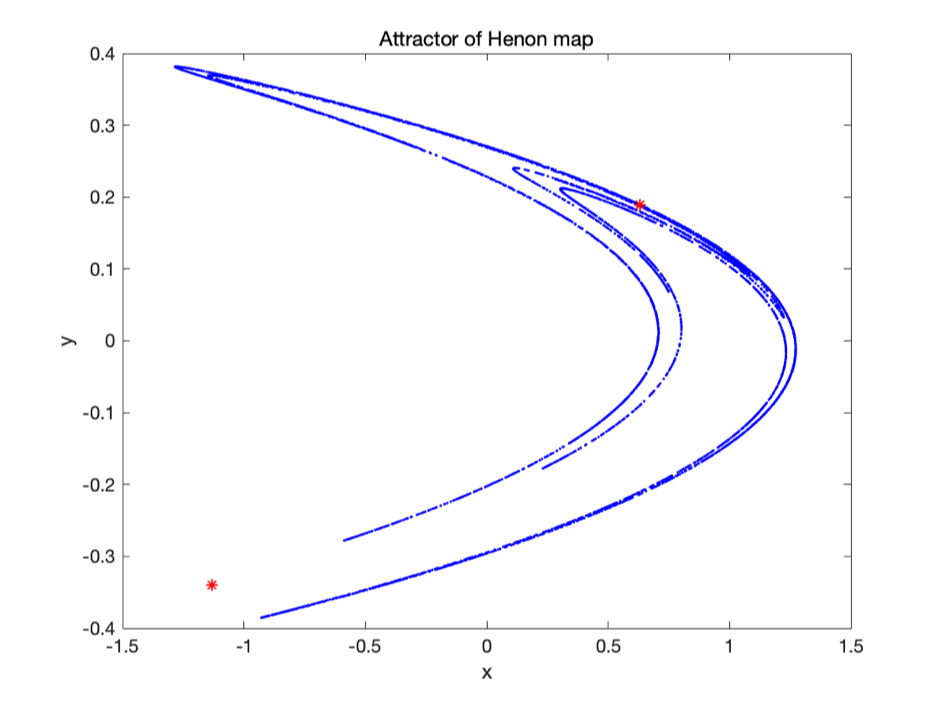
\includegraphics[scale=0.8]{henon_phase.png}
    \caption{埃农映射的吸引子和不动点($a=1.4,b=0.3$)}
    \label{fig:logi_lypn}
\end{figure}

在我们的Koopman分析中,我们在取上述参数值的情况下,通过Henon映射的迭代方程演化出一系列的数据,作为Koopman分析的源数据,以此来分析Henon映射的系统特征。


\subsection{埃农映射的Koopman算符本征函数}
\subsubsection{正交完备基函数空间}
\begin{figure}
    \centering
    \subfloat[高斯基函数]{
      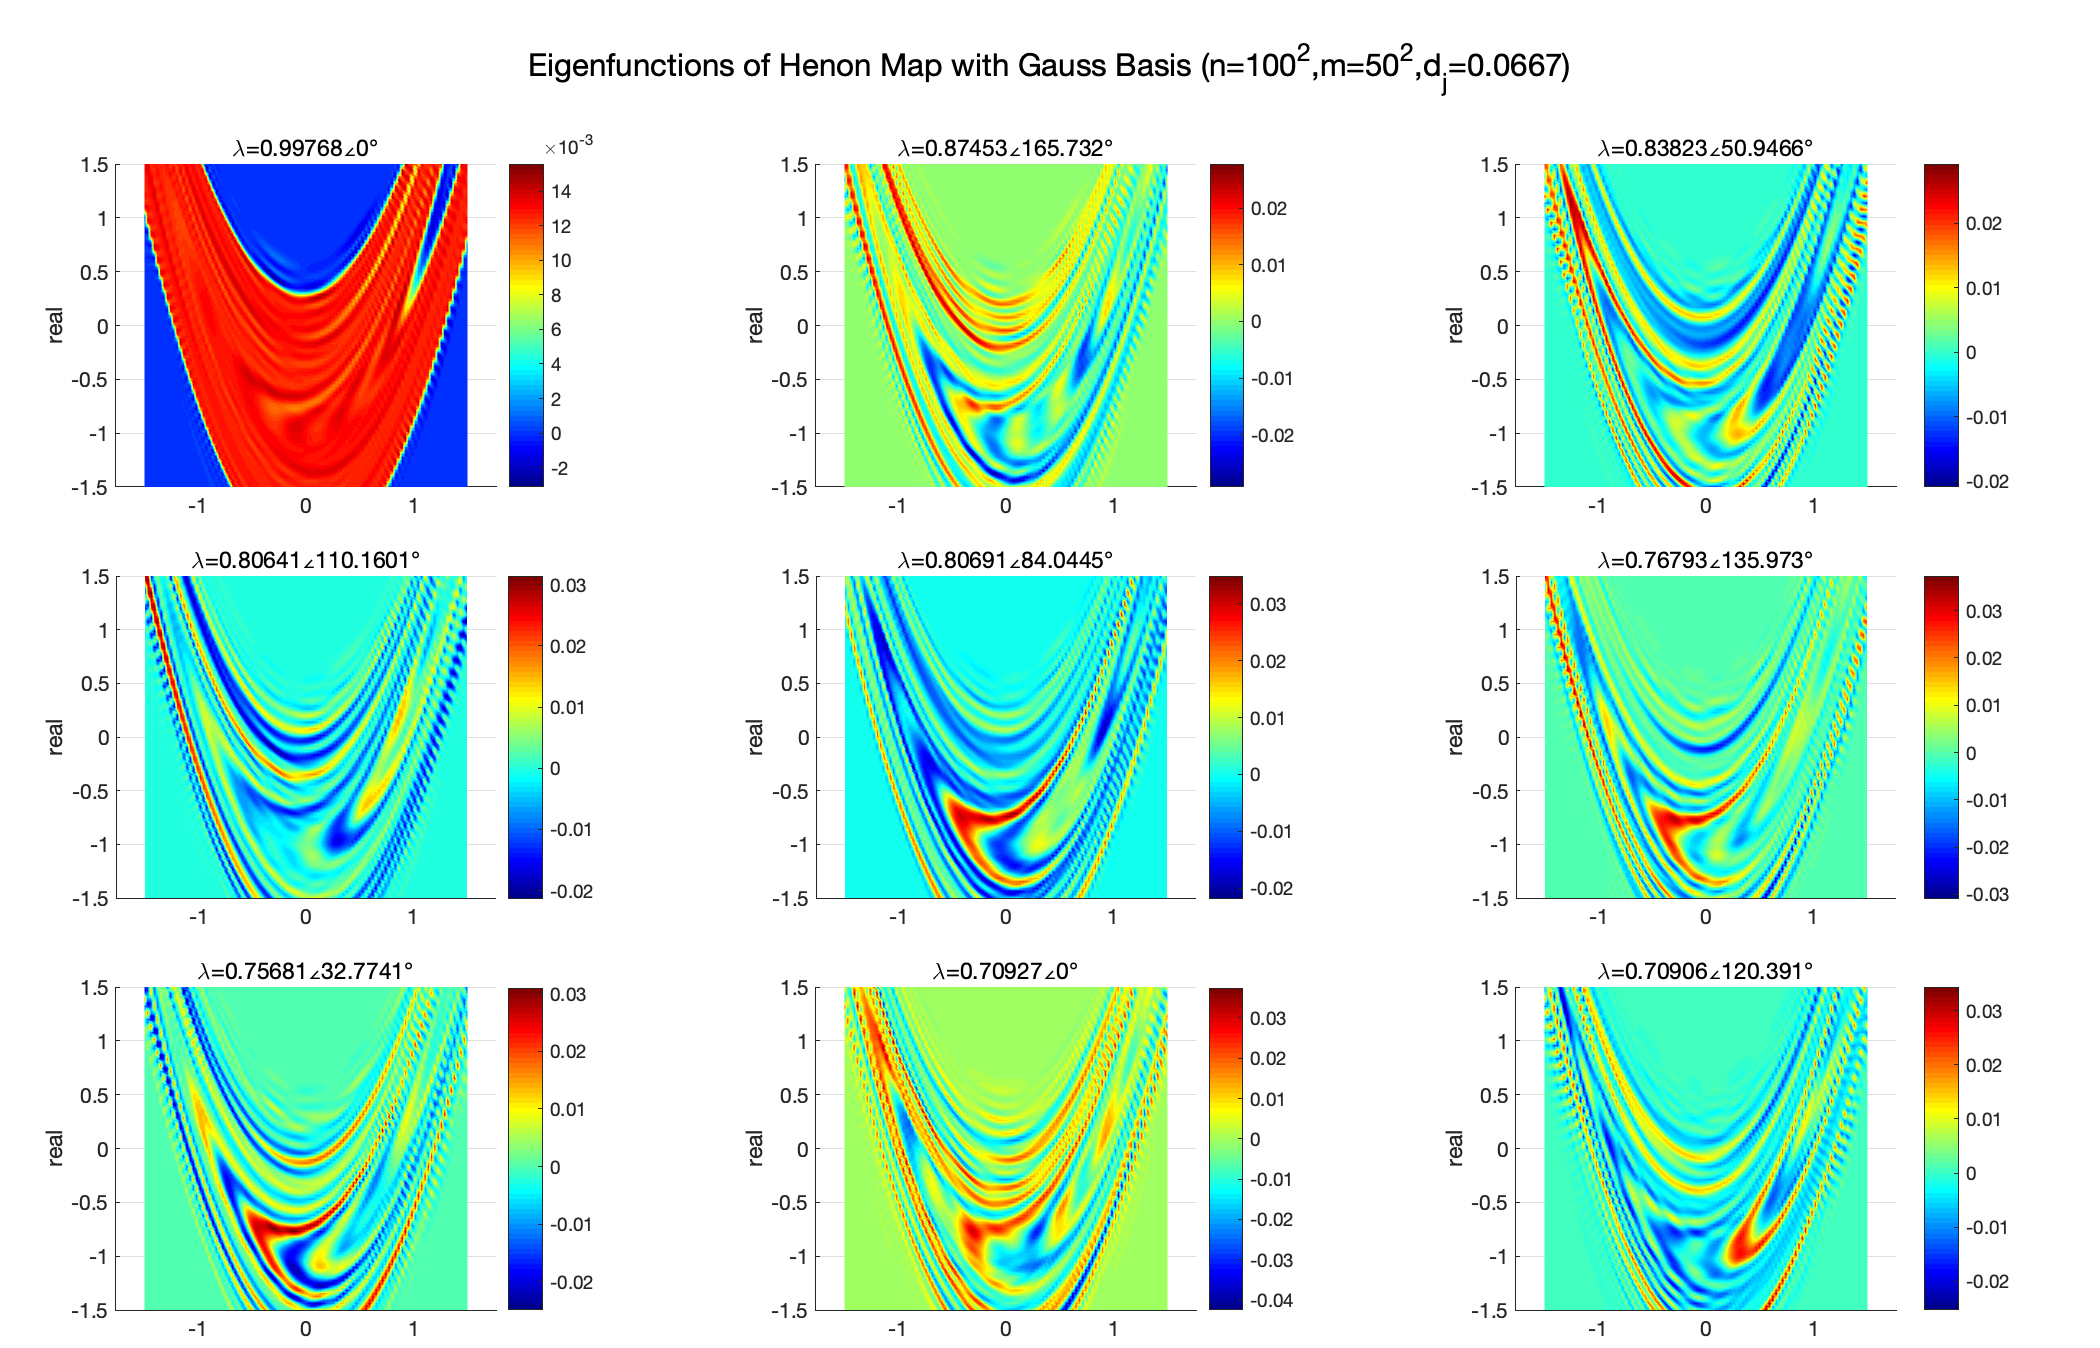
\includegraphics[scale=0.4]{henon/Henon_eigen_Gauss_n100m50md45}}
    \\
    \subfloat[傅里叶基函数]{
      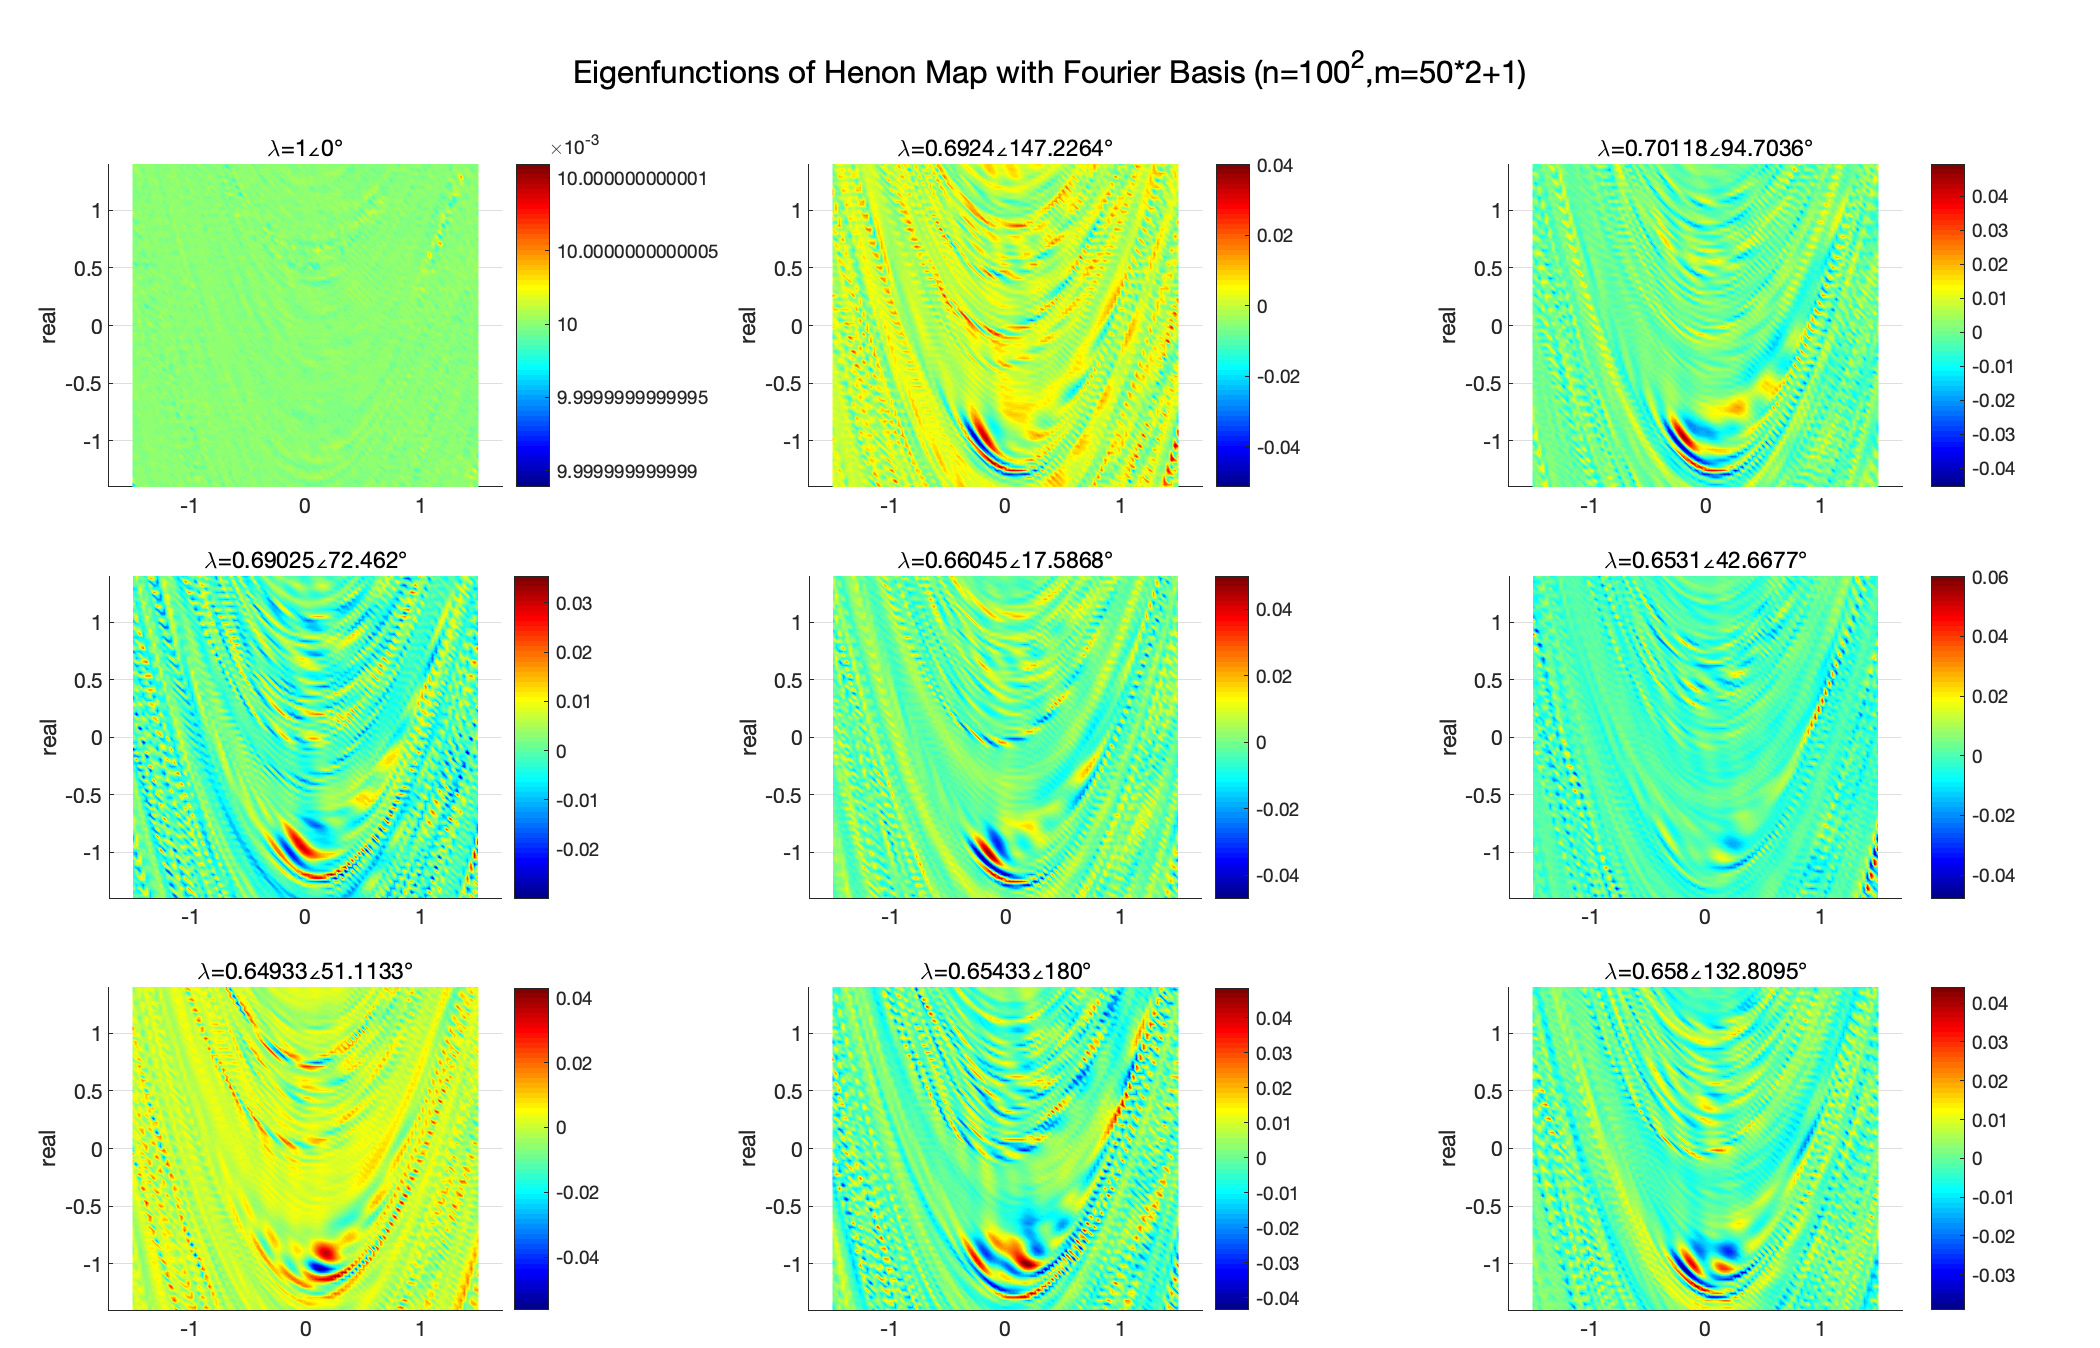
\includegraphics[scale=0.4]{henon/Henon_eigen_Fourier_n100m50}}
    \caption{埃农映射不同基函数的本征函数}
\end{figure}

\begin{figure}
    \centering
    \subfloat{
      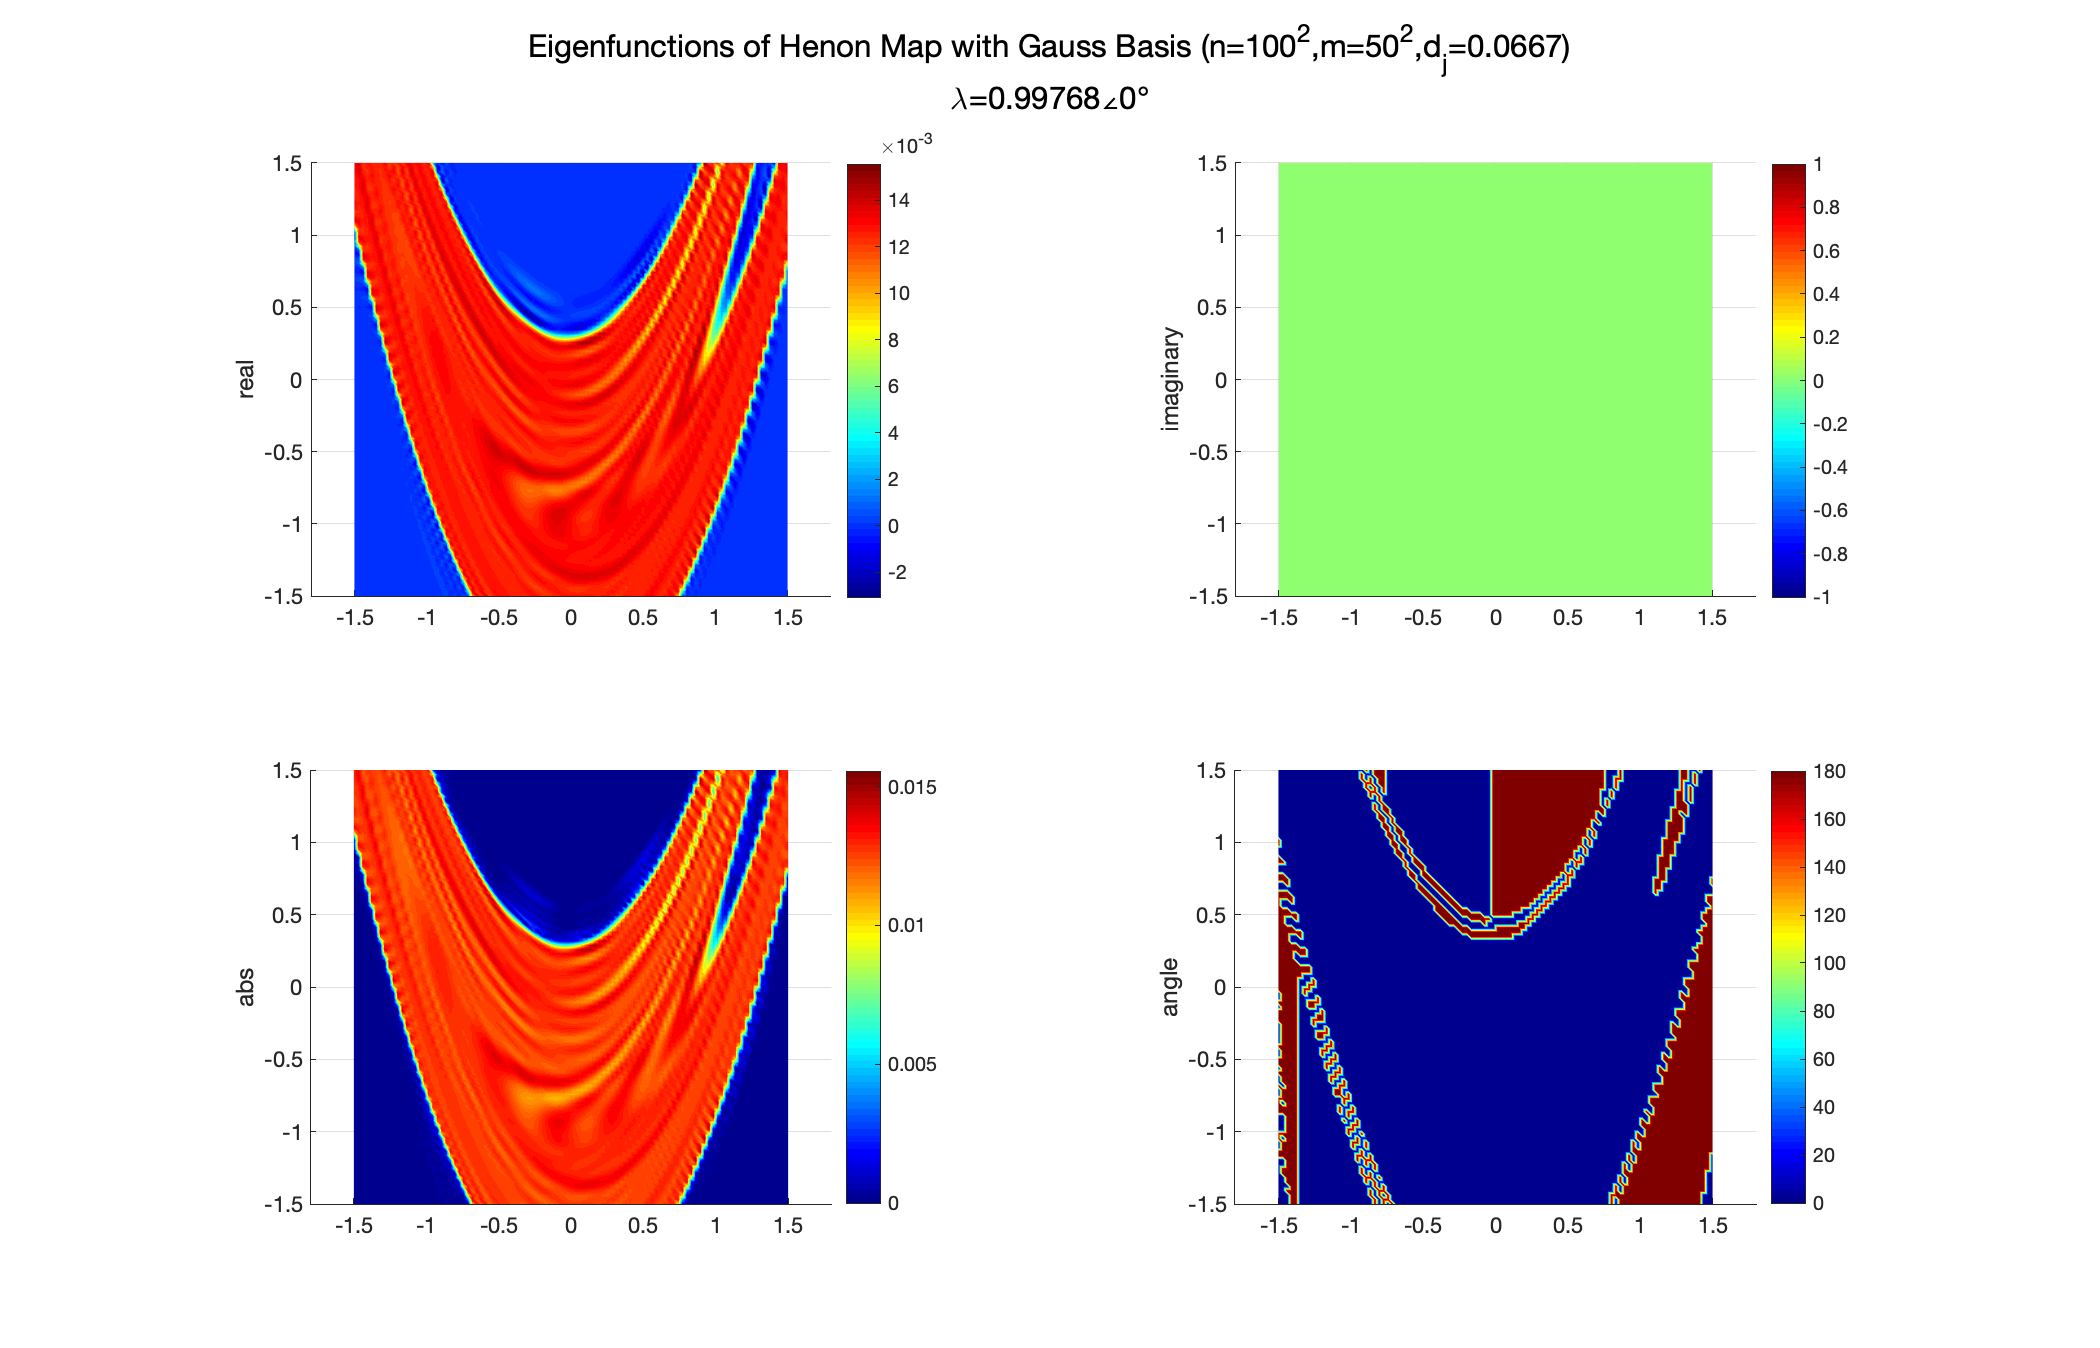
\includegraphics[scale=0.2]{henon/Henon_eigen_Gauss_n100m50md45_figure1}}
    \subfloat{
      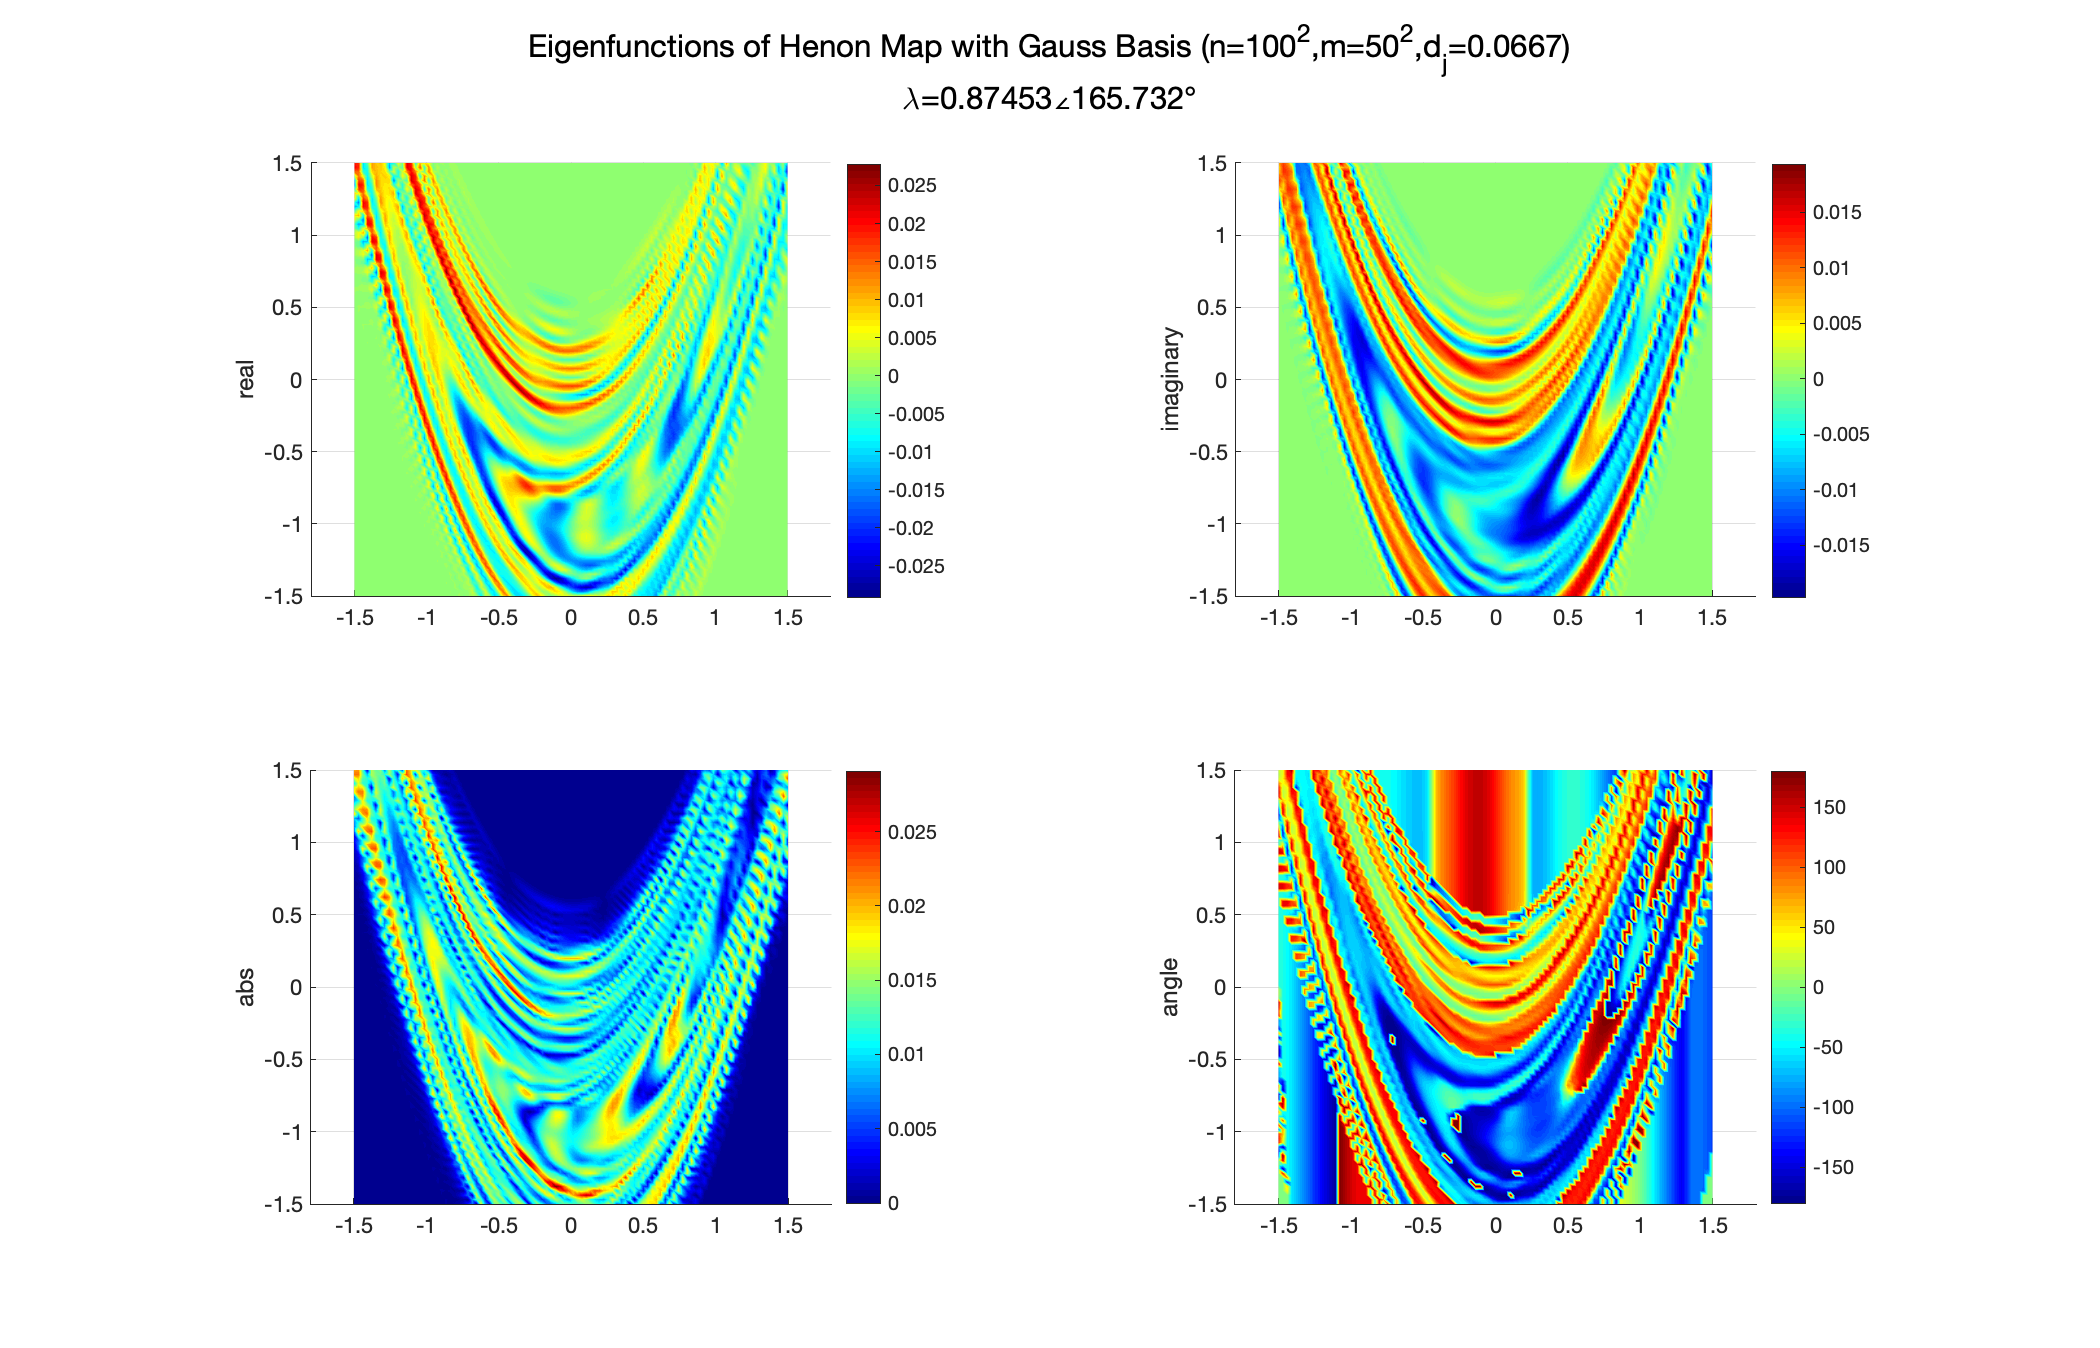
\includegraphics[scale=0.2]{henon/Henon_eigen_Gauss_n100m50md45_figure2}}
    \\
    \subfloat{
      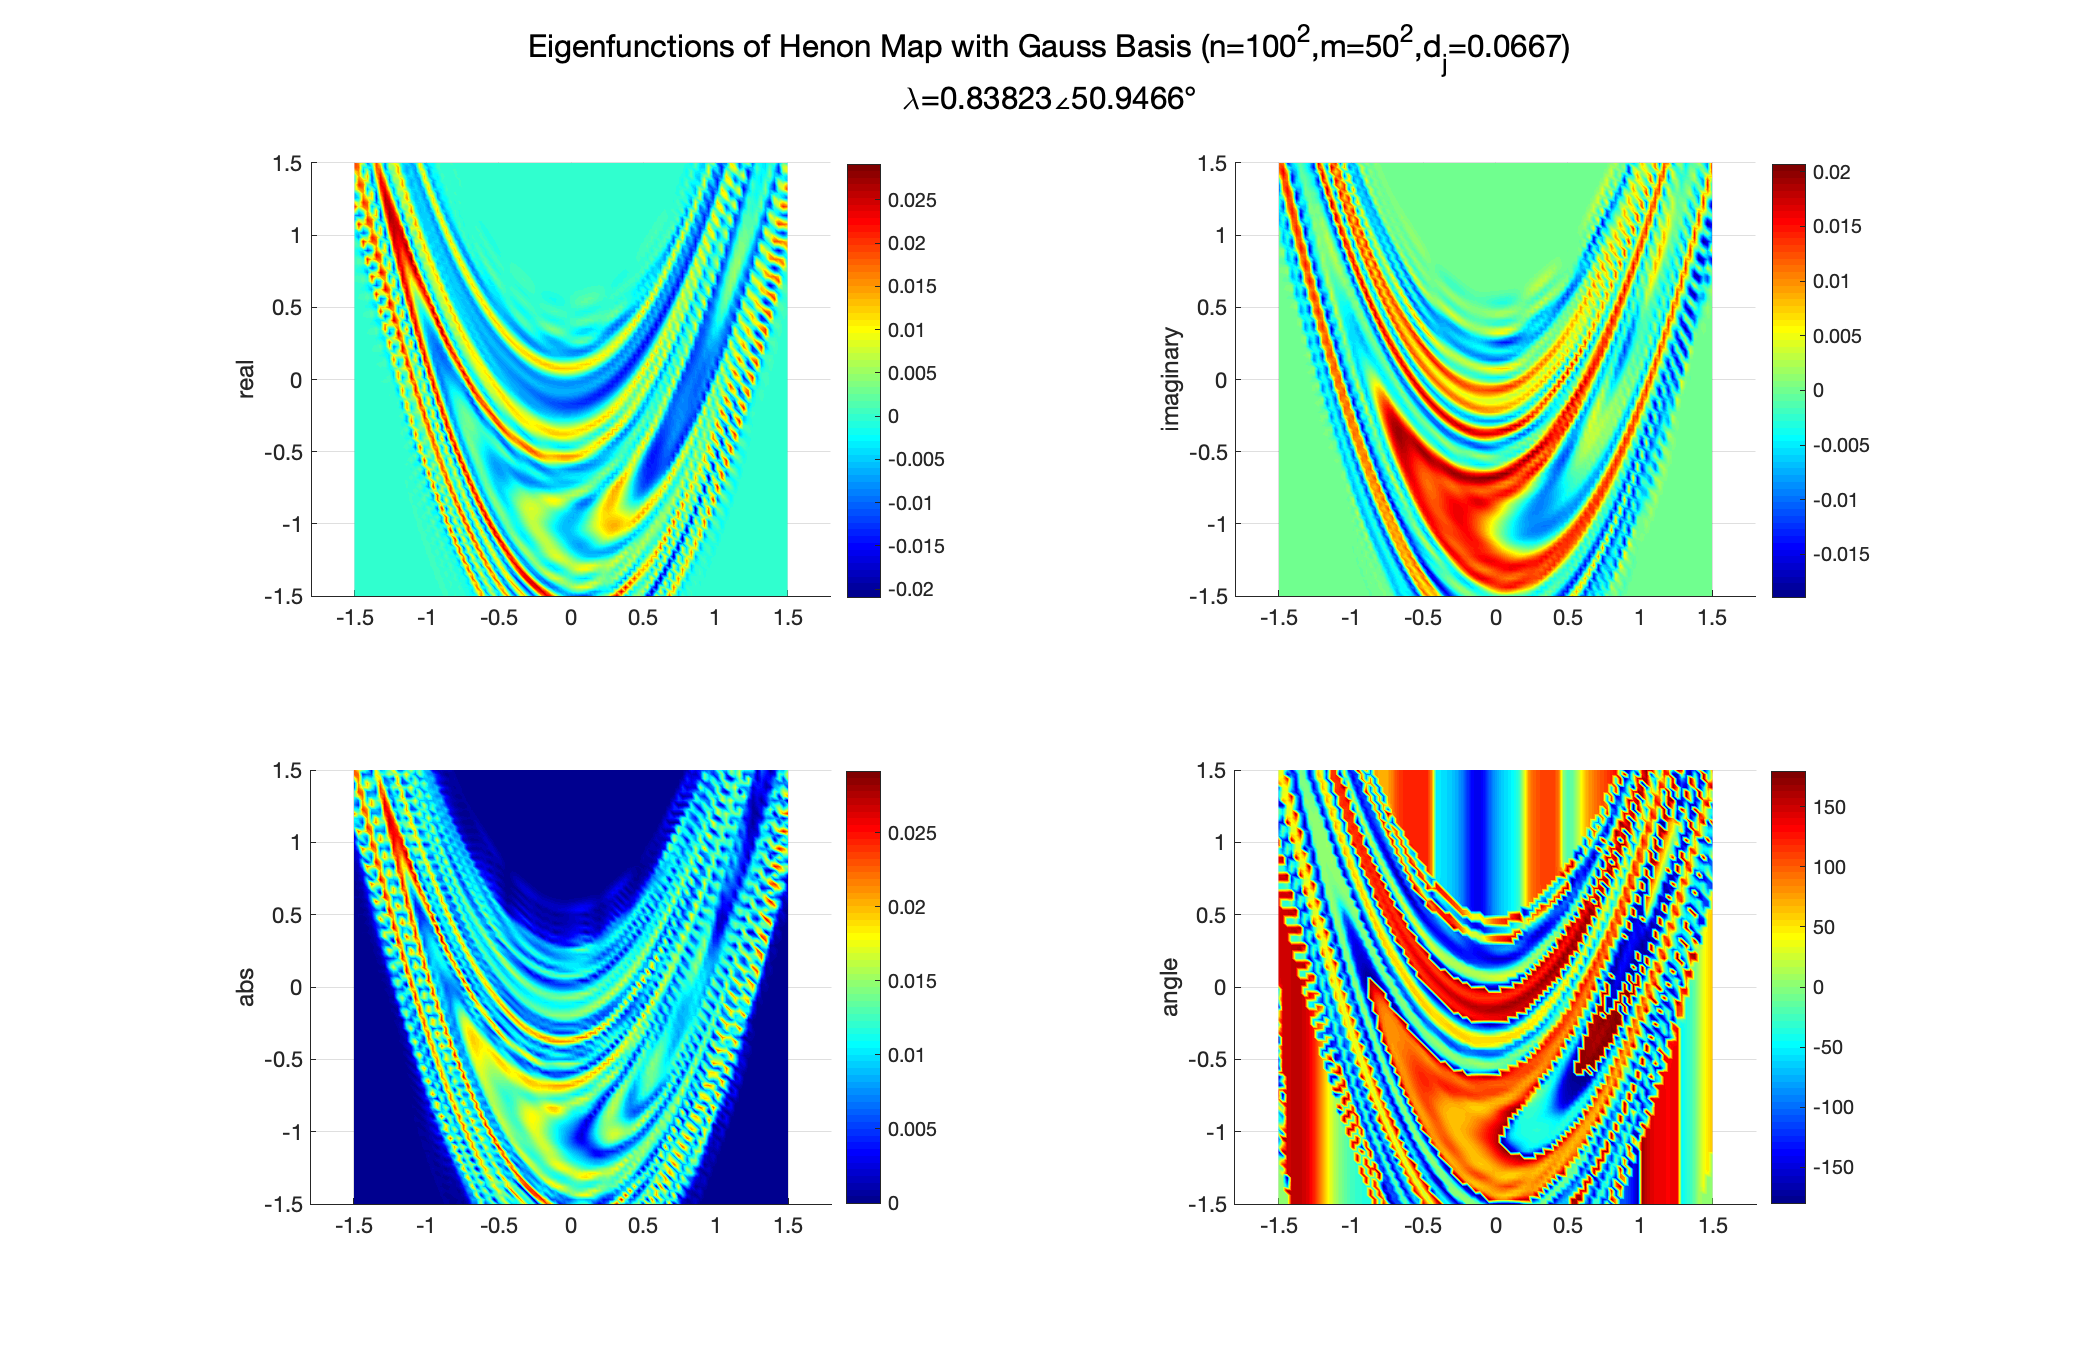
\includegraphics[scale=0.2]{henon/Henon_eigen_Gauss_n100m50md45_figure3}}
    \subfloat{
      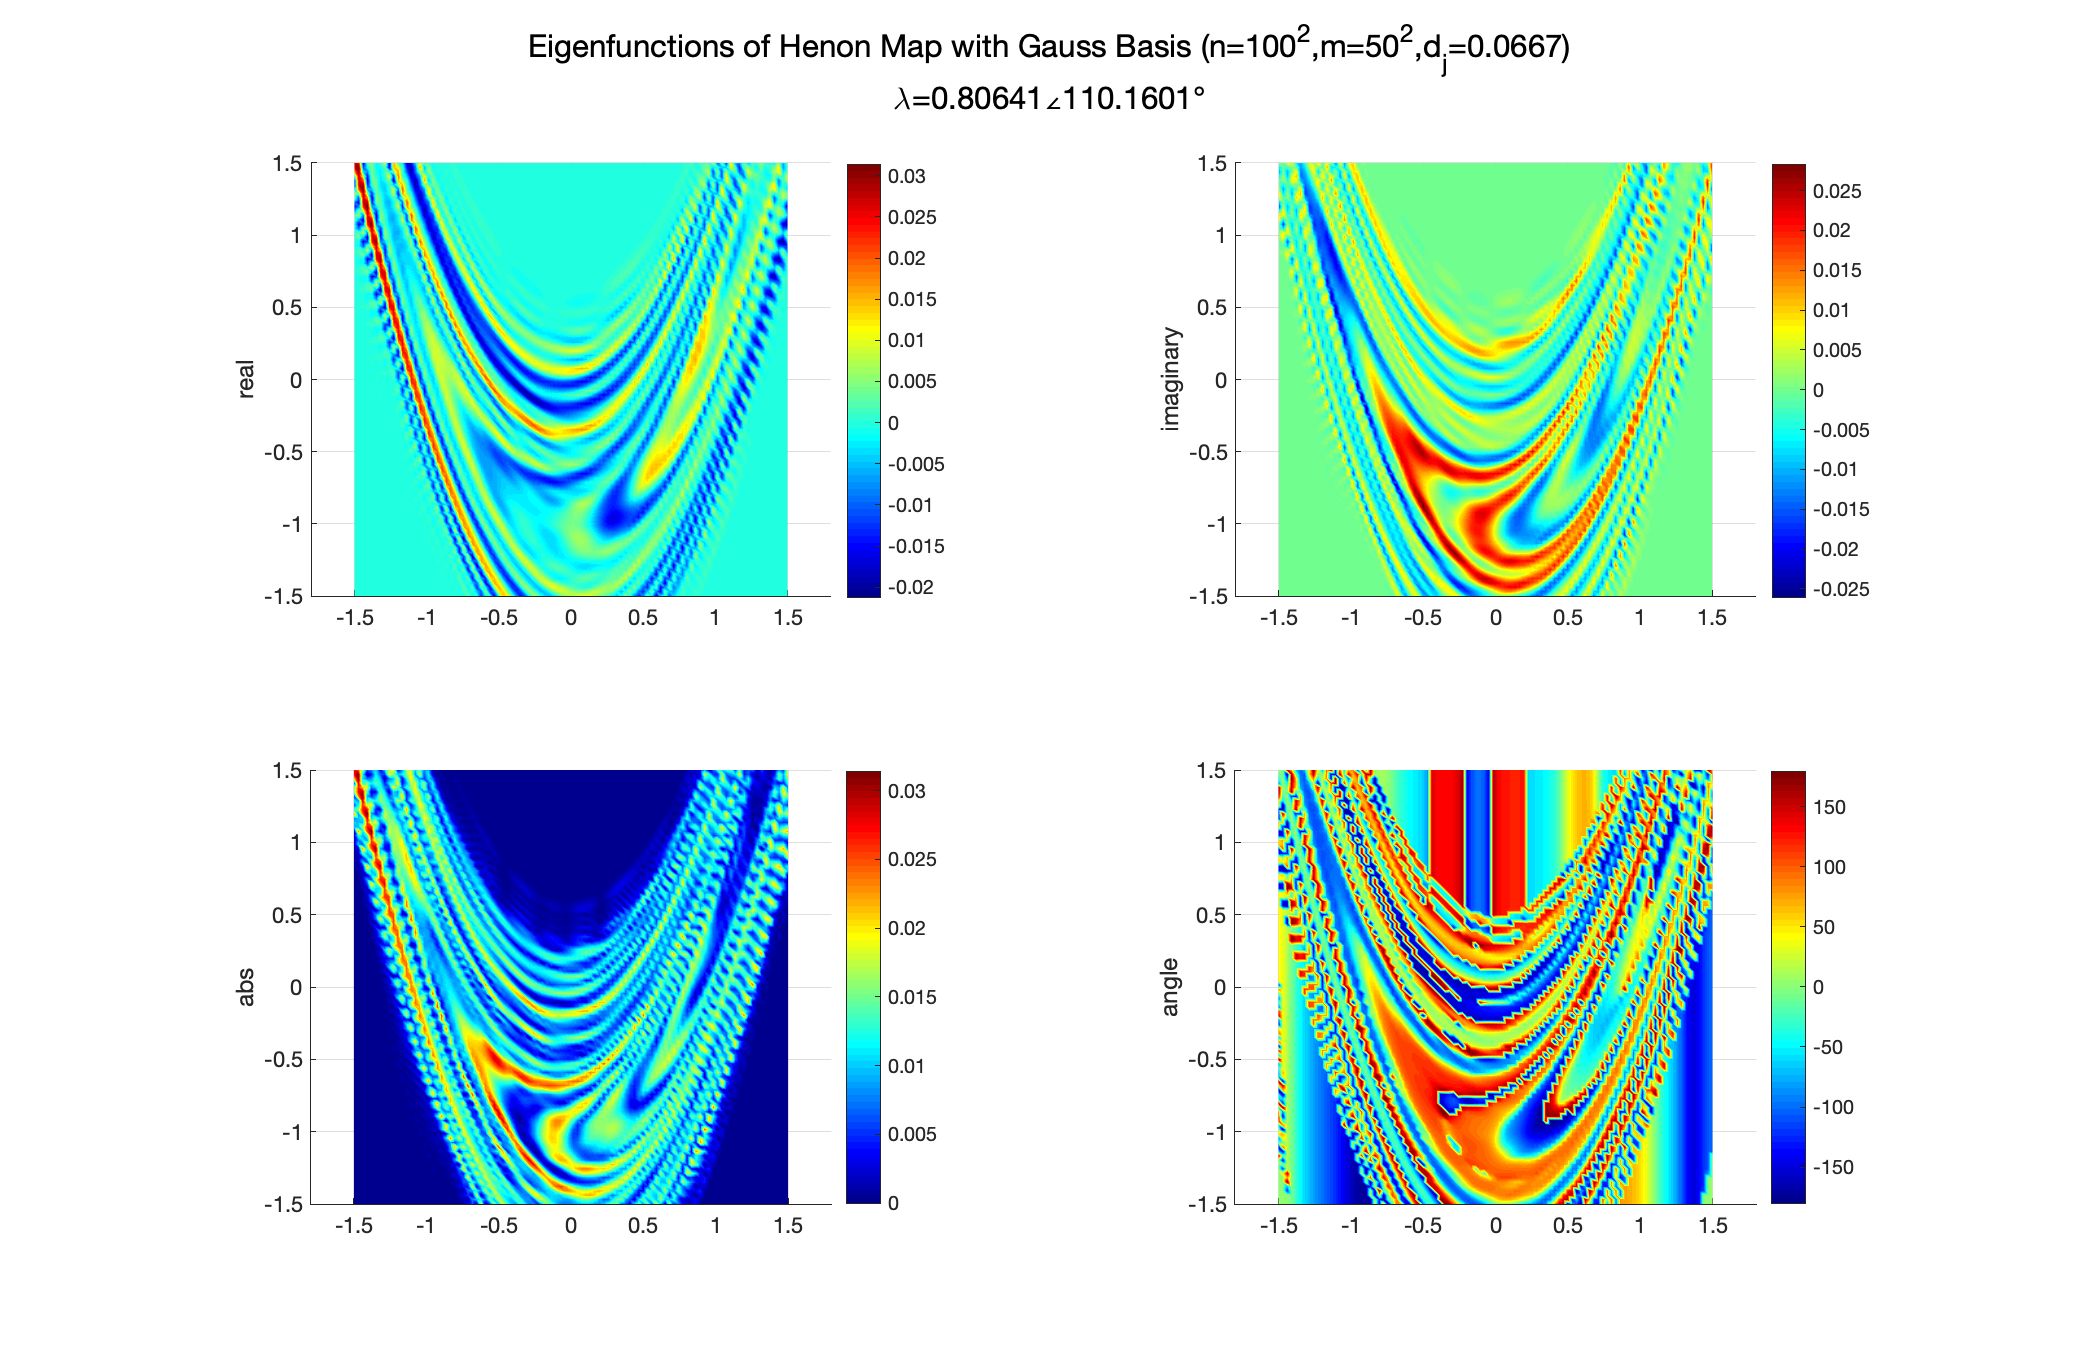
\includegraphics[scale=0.2]{henon/Henon_eigen_Gauss_n100m50md45_figure4}}
    \\
    \subfloat{
      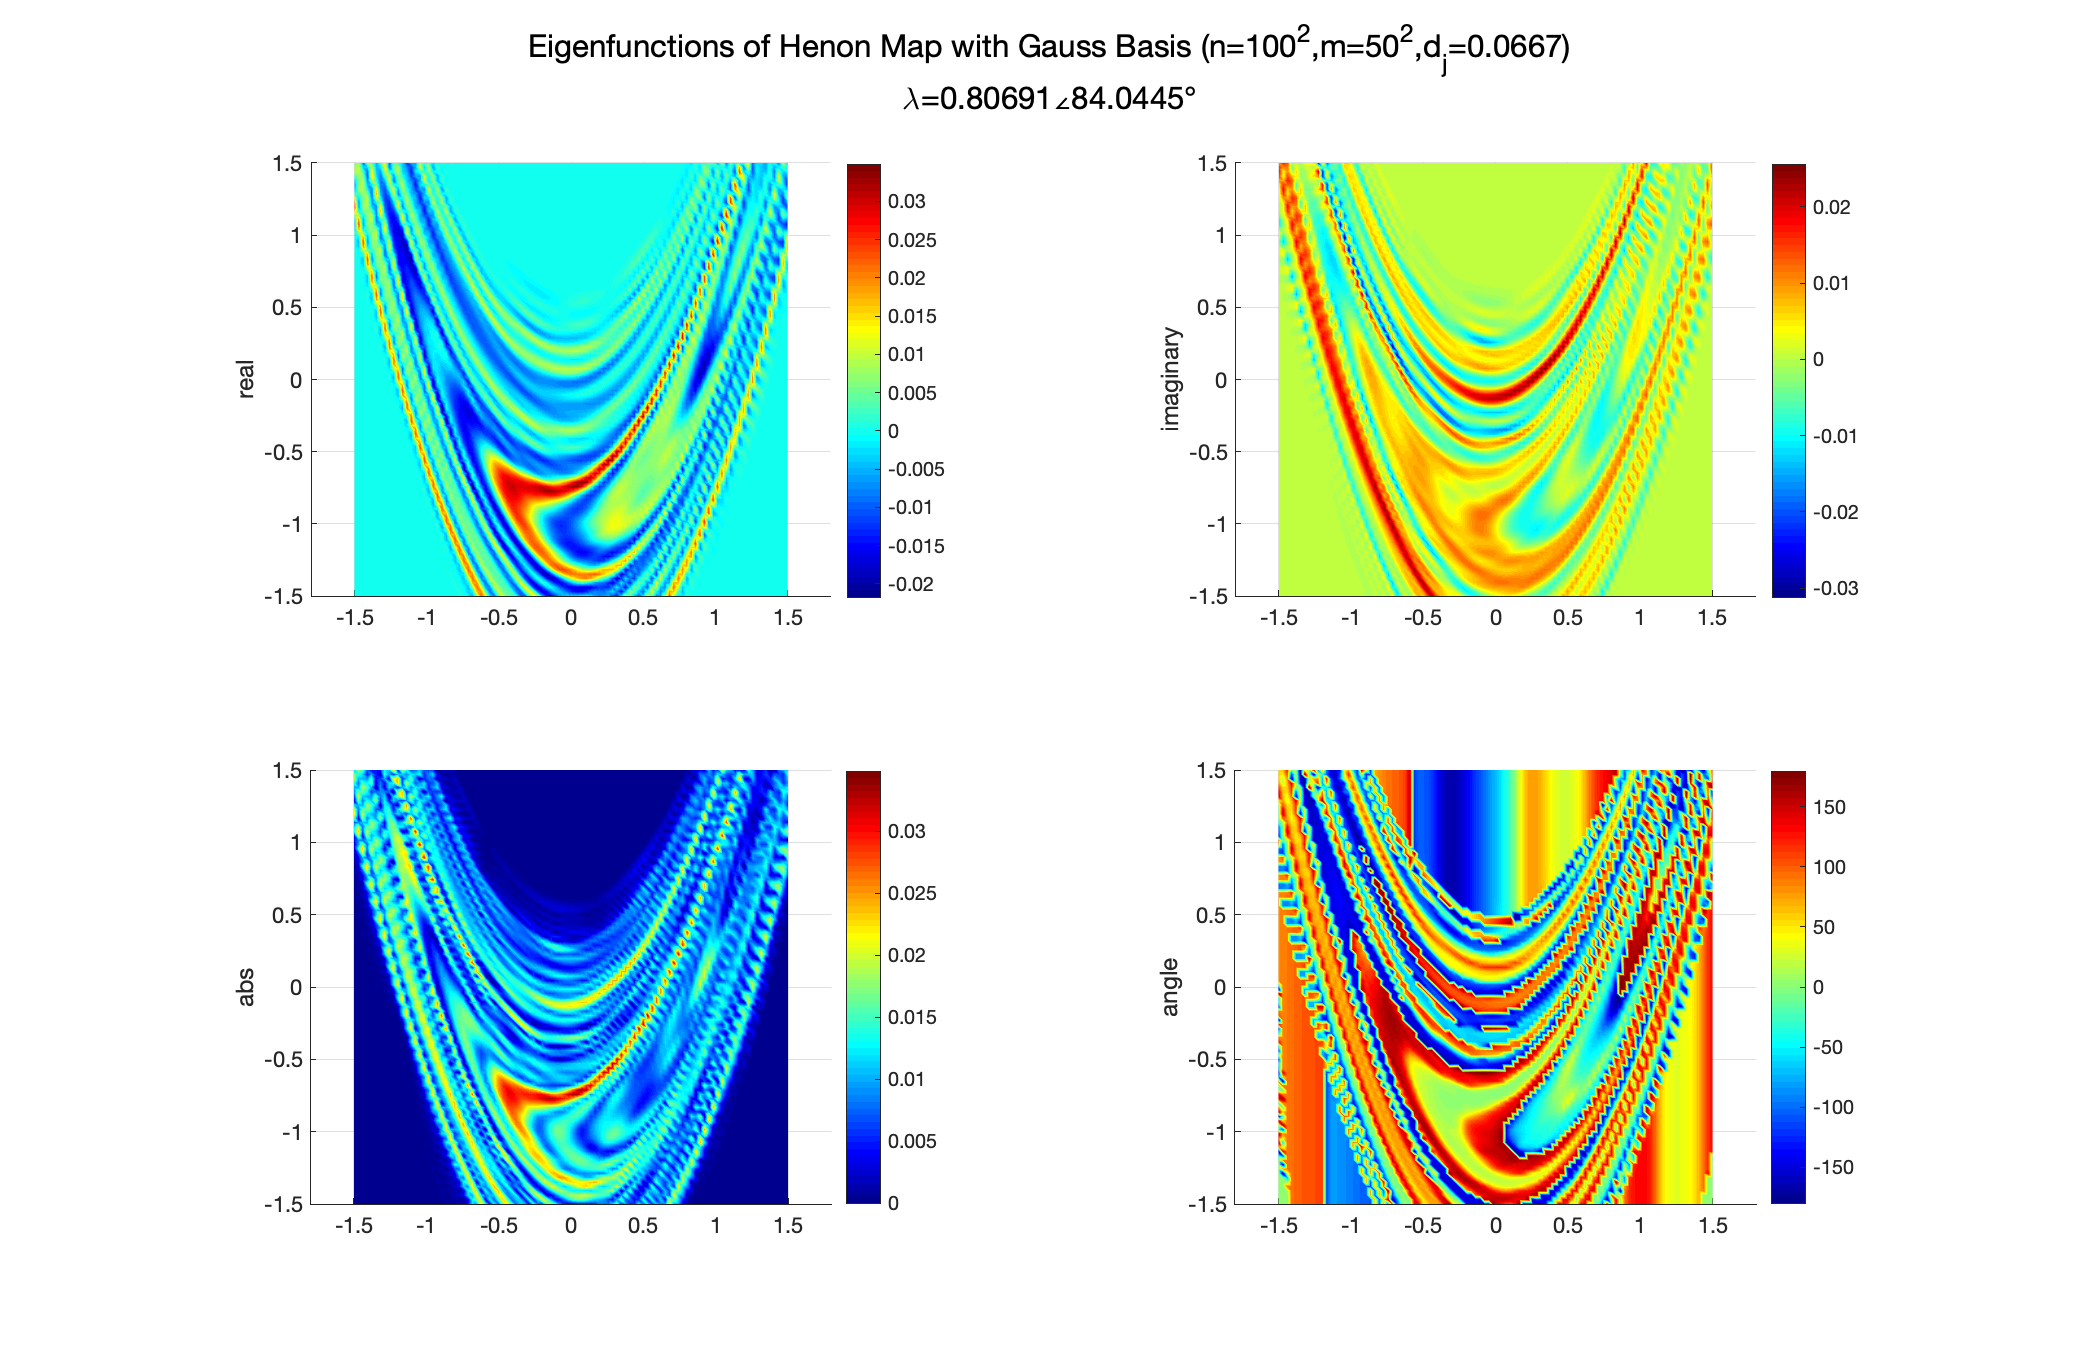
\includegraphics[scale=0.2]{henon/Henon_eigen_Gauss_n100m50md45_figure5}}
    \subfloat{
      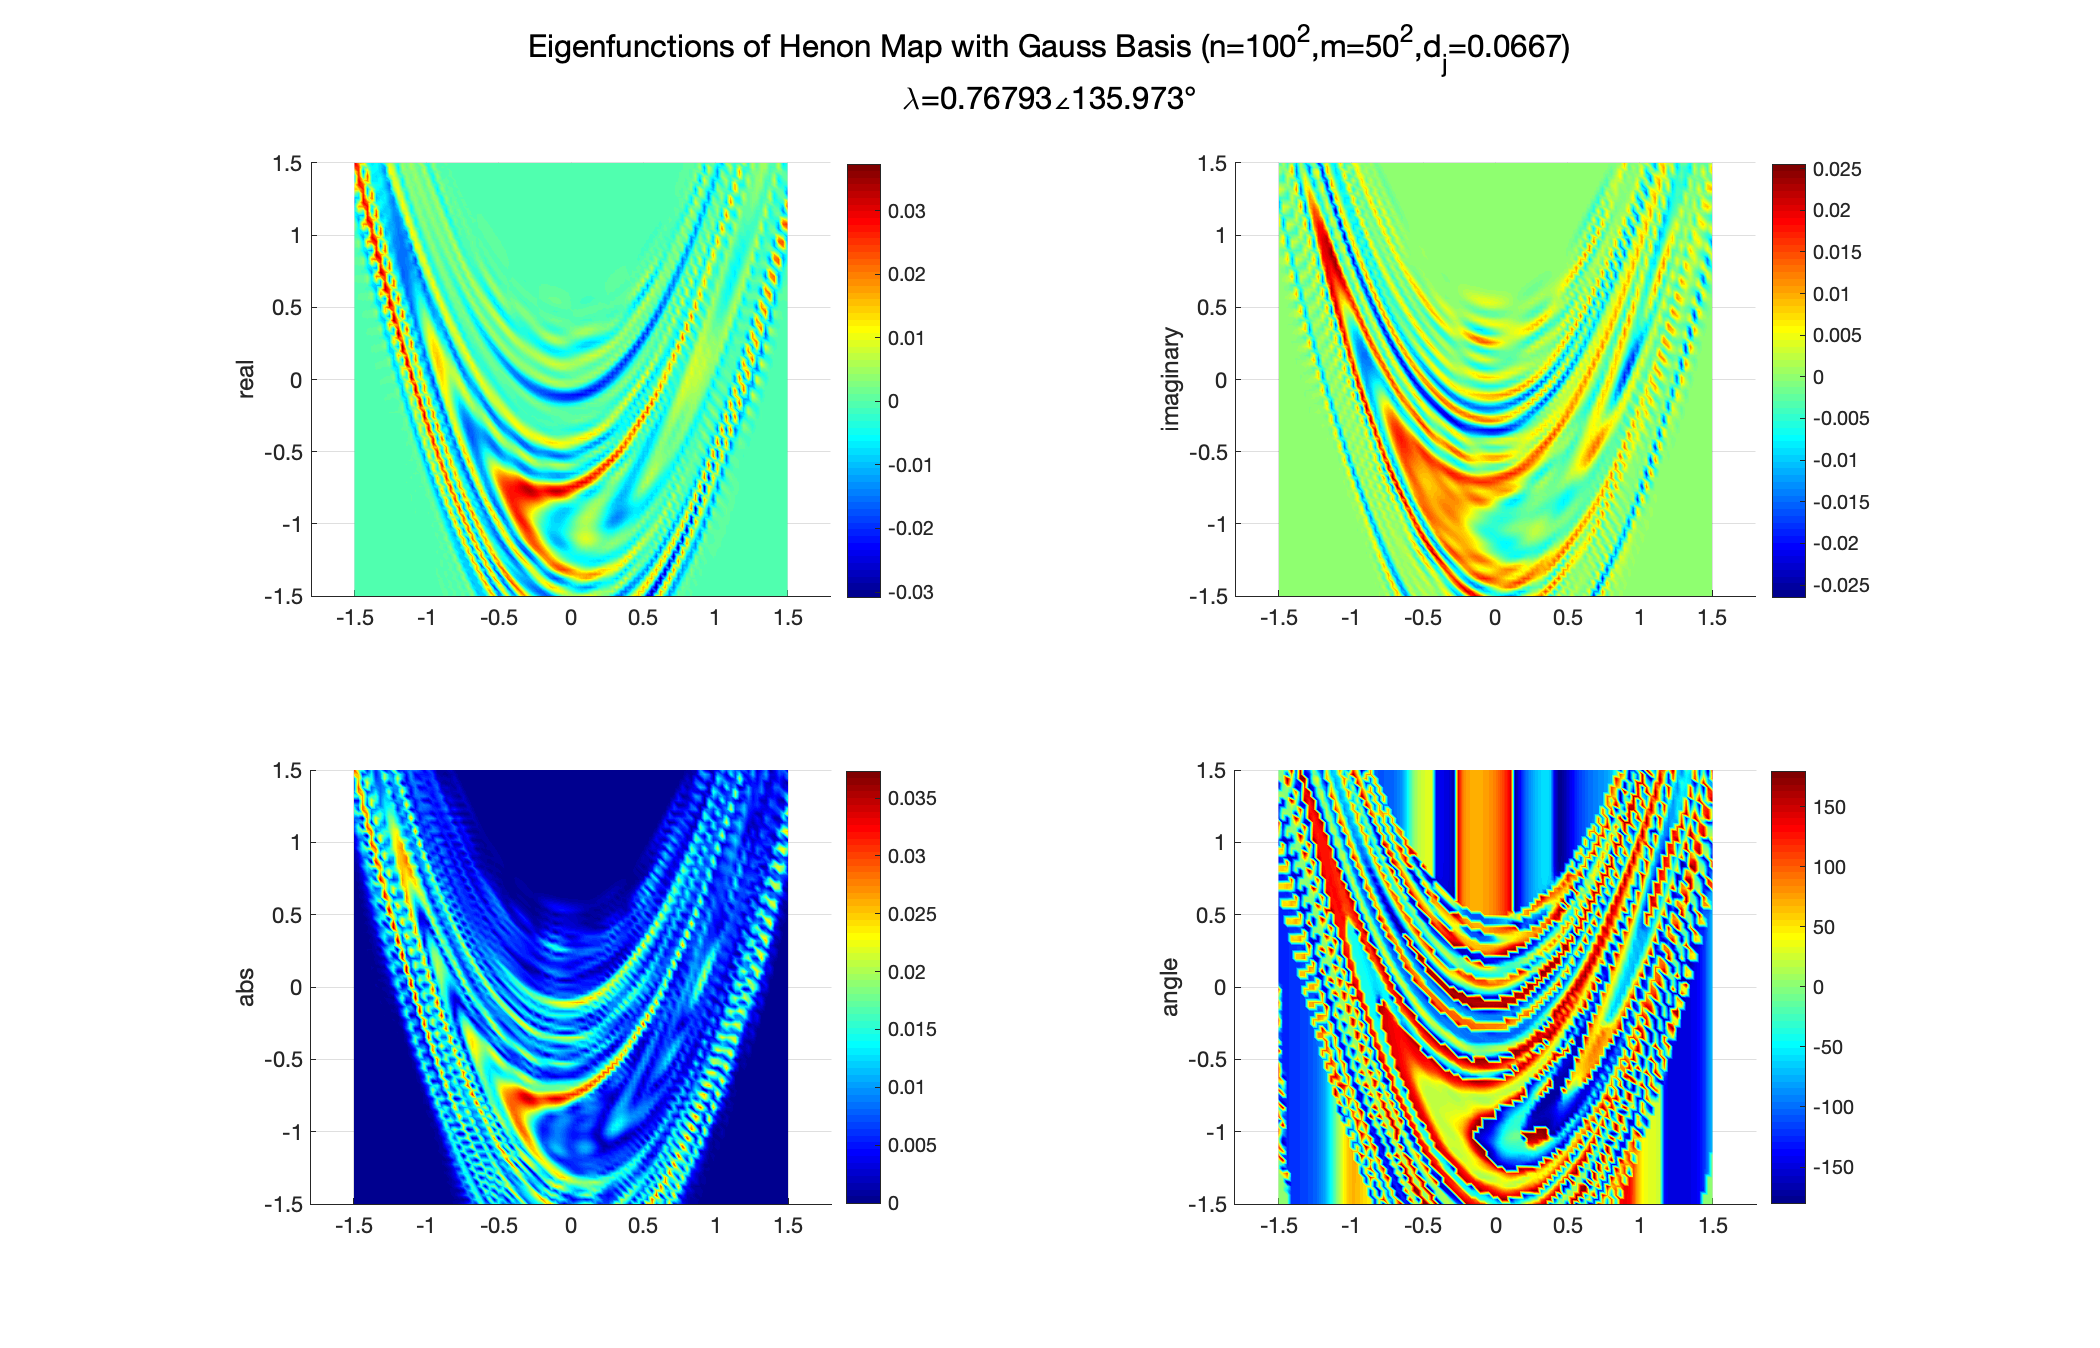
\includegraphics[scale=0.2]{henon/Henon_eigen_Gauss_n100m50md45_figure6}}
    \\
    \subfloat{
      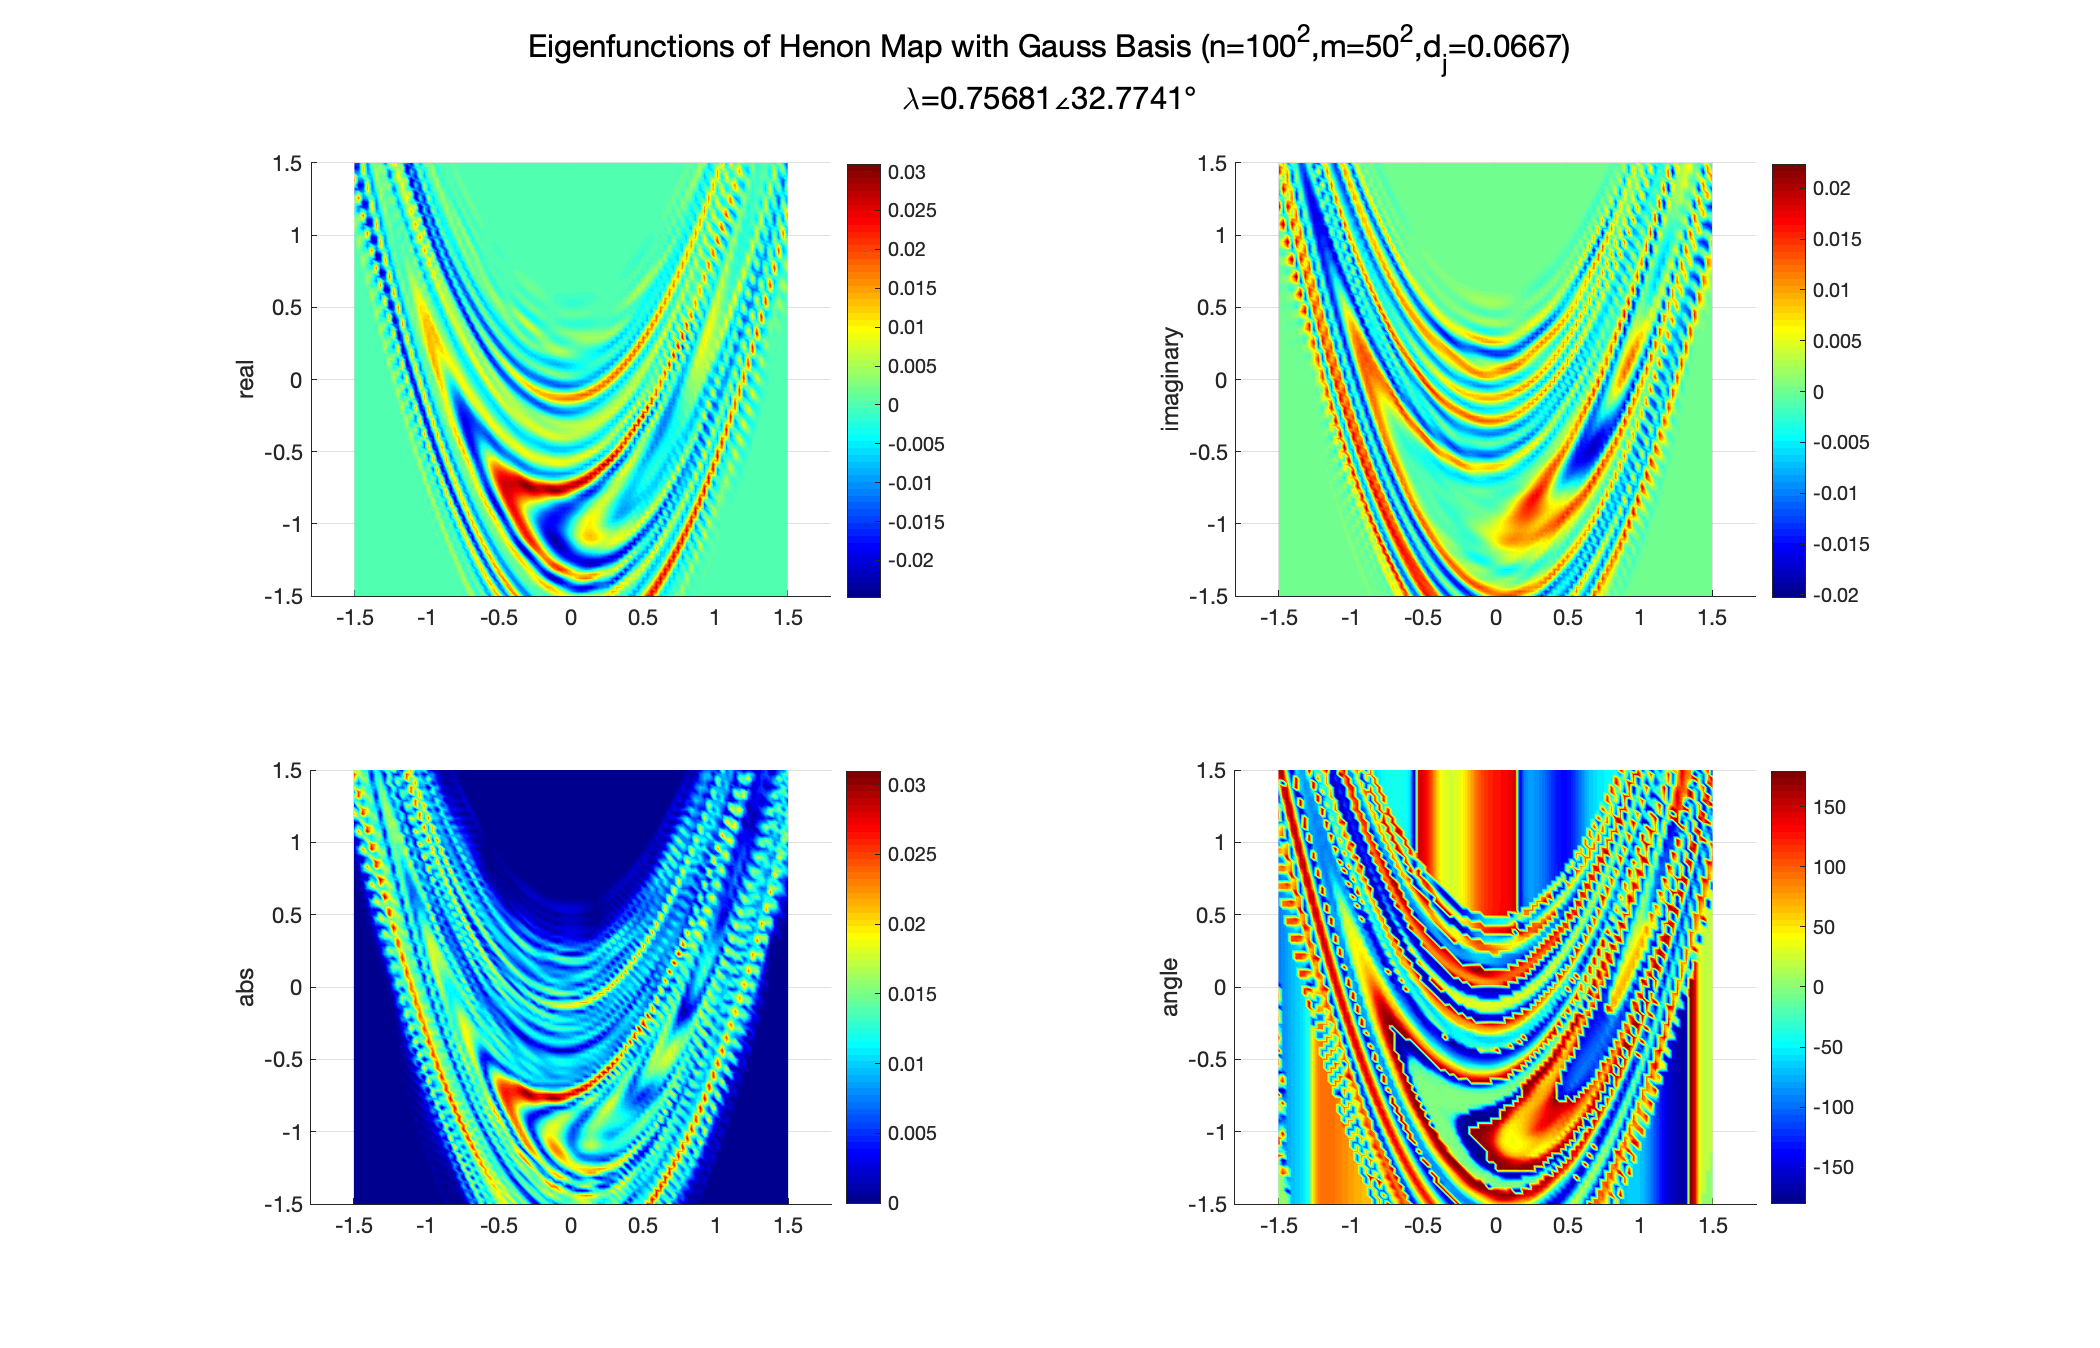
\includegraphics[scale=0.2]{henon/Henon_eigen_Gauss_n100m50md45_figure7}}
    \subfloat{
      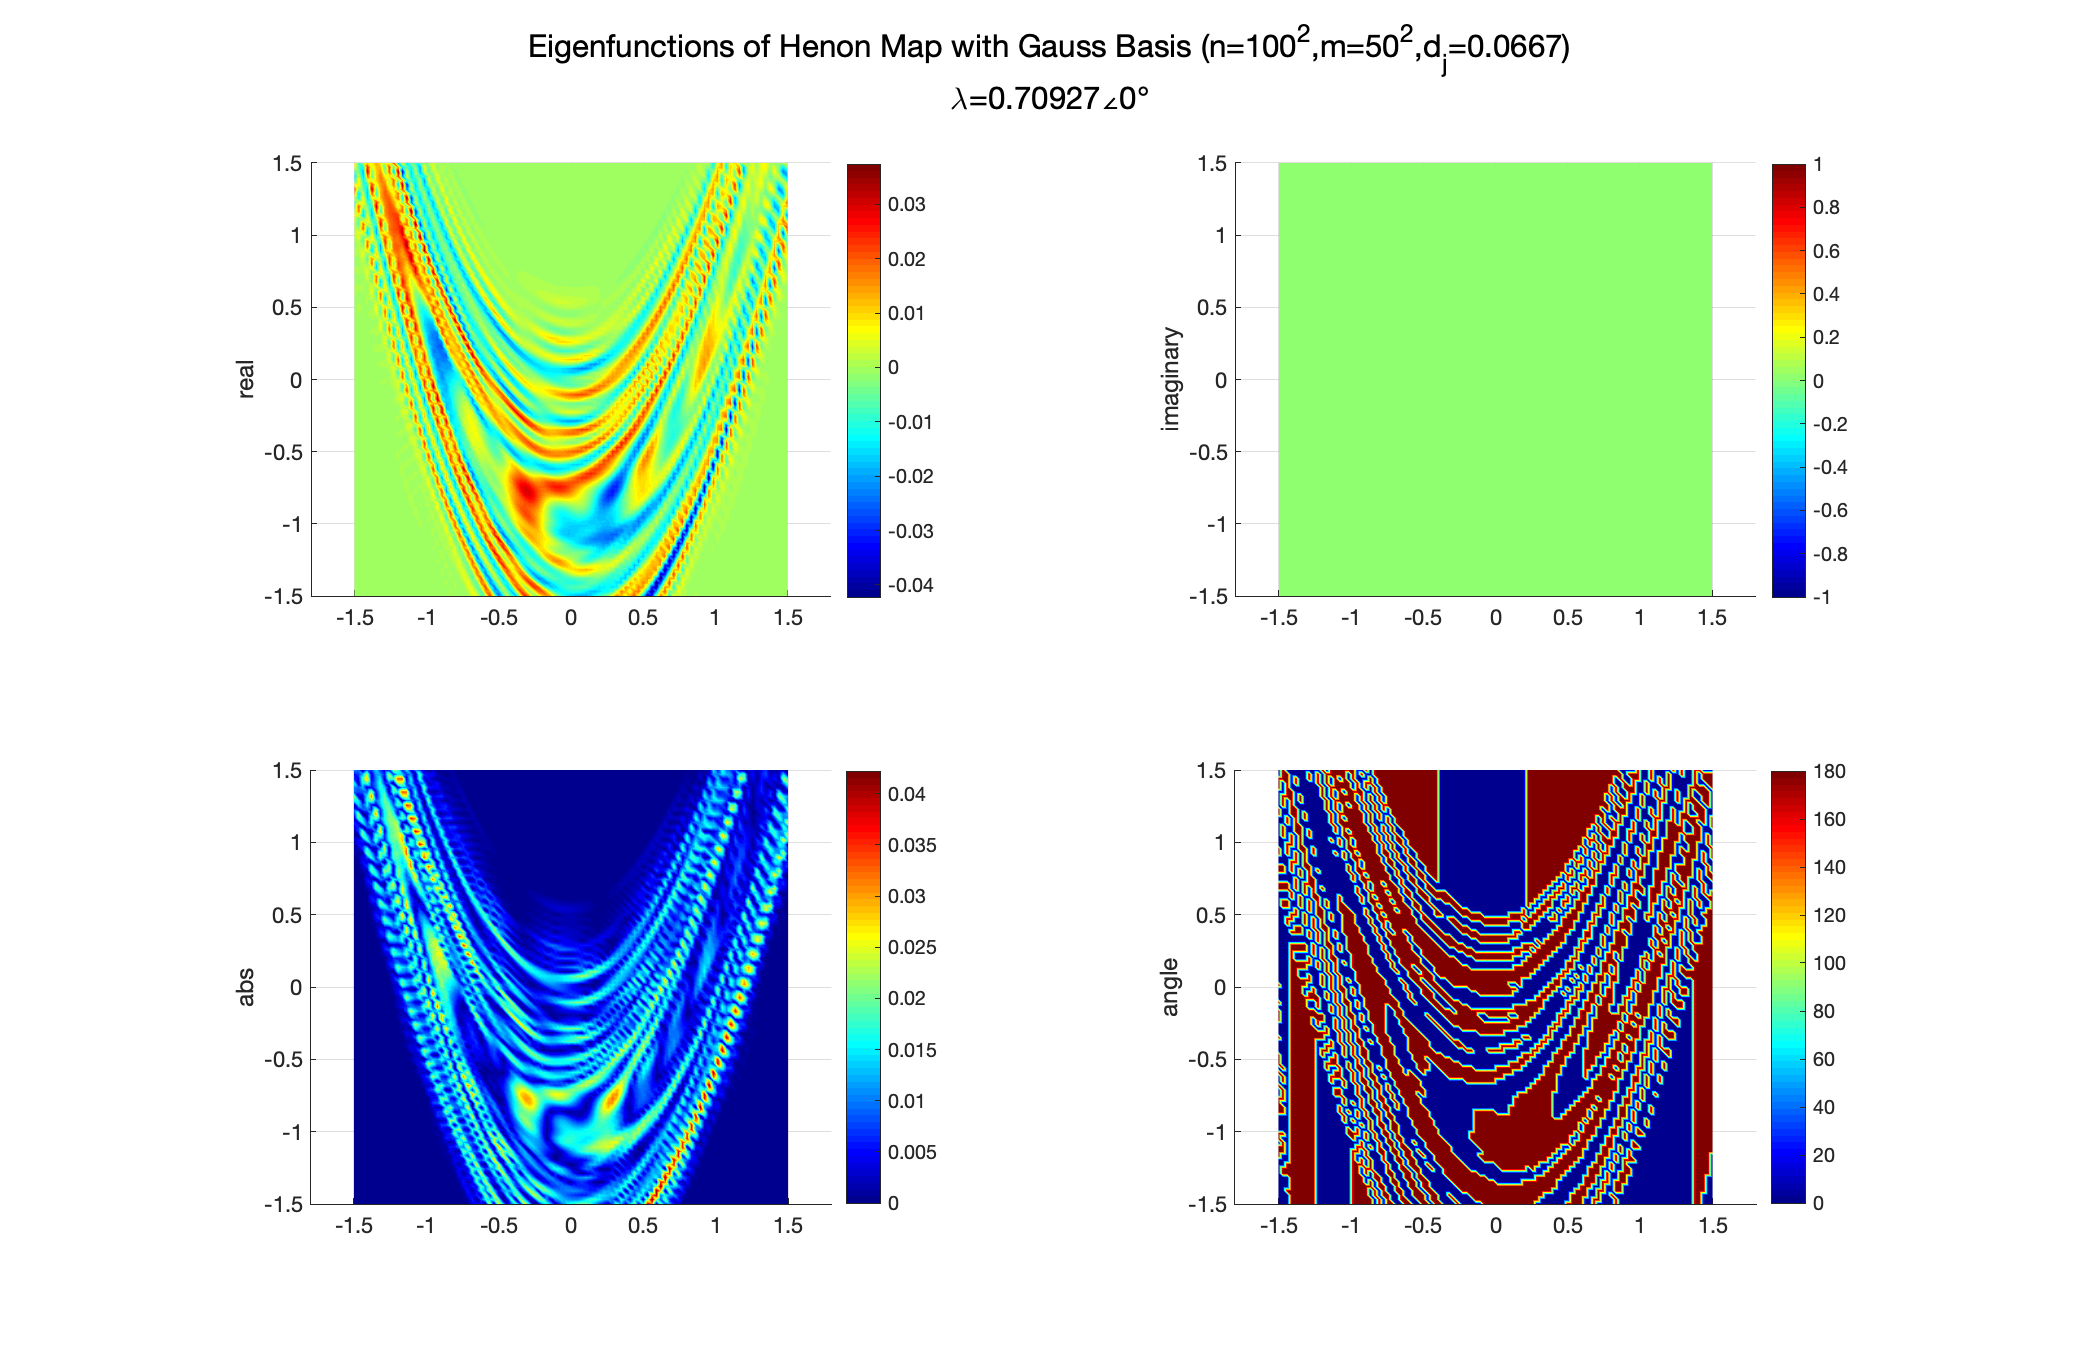
\includegraphics[scale=0.2]{henon/Henon_eigen_Gauss_n100m50md45_figure8}}
    \\
    \caption{埃农映射不同本征值的本征函数($n=100^2$,$m=50^2,d_j=\frac{3}{45}$)}
\end{figure}

\subsubsection{自然基函数空间}
\begin{figure}
    \centering
    \subfloat{
      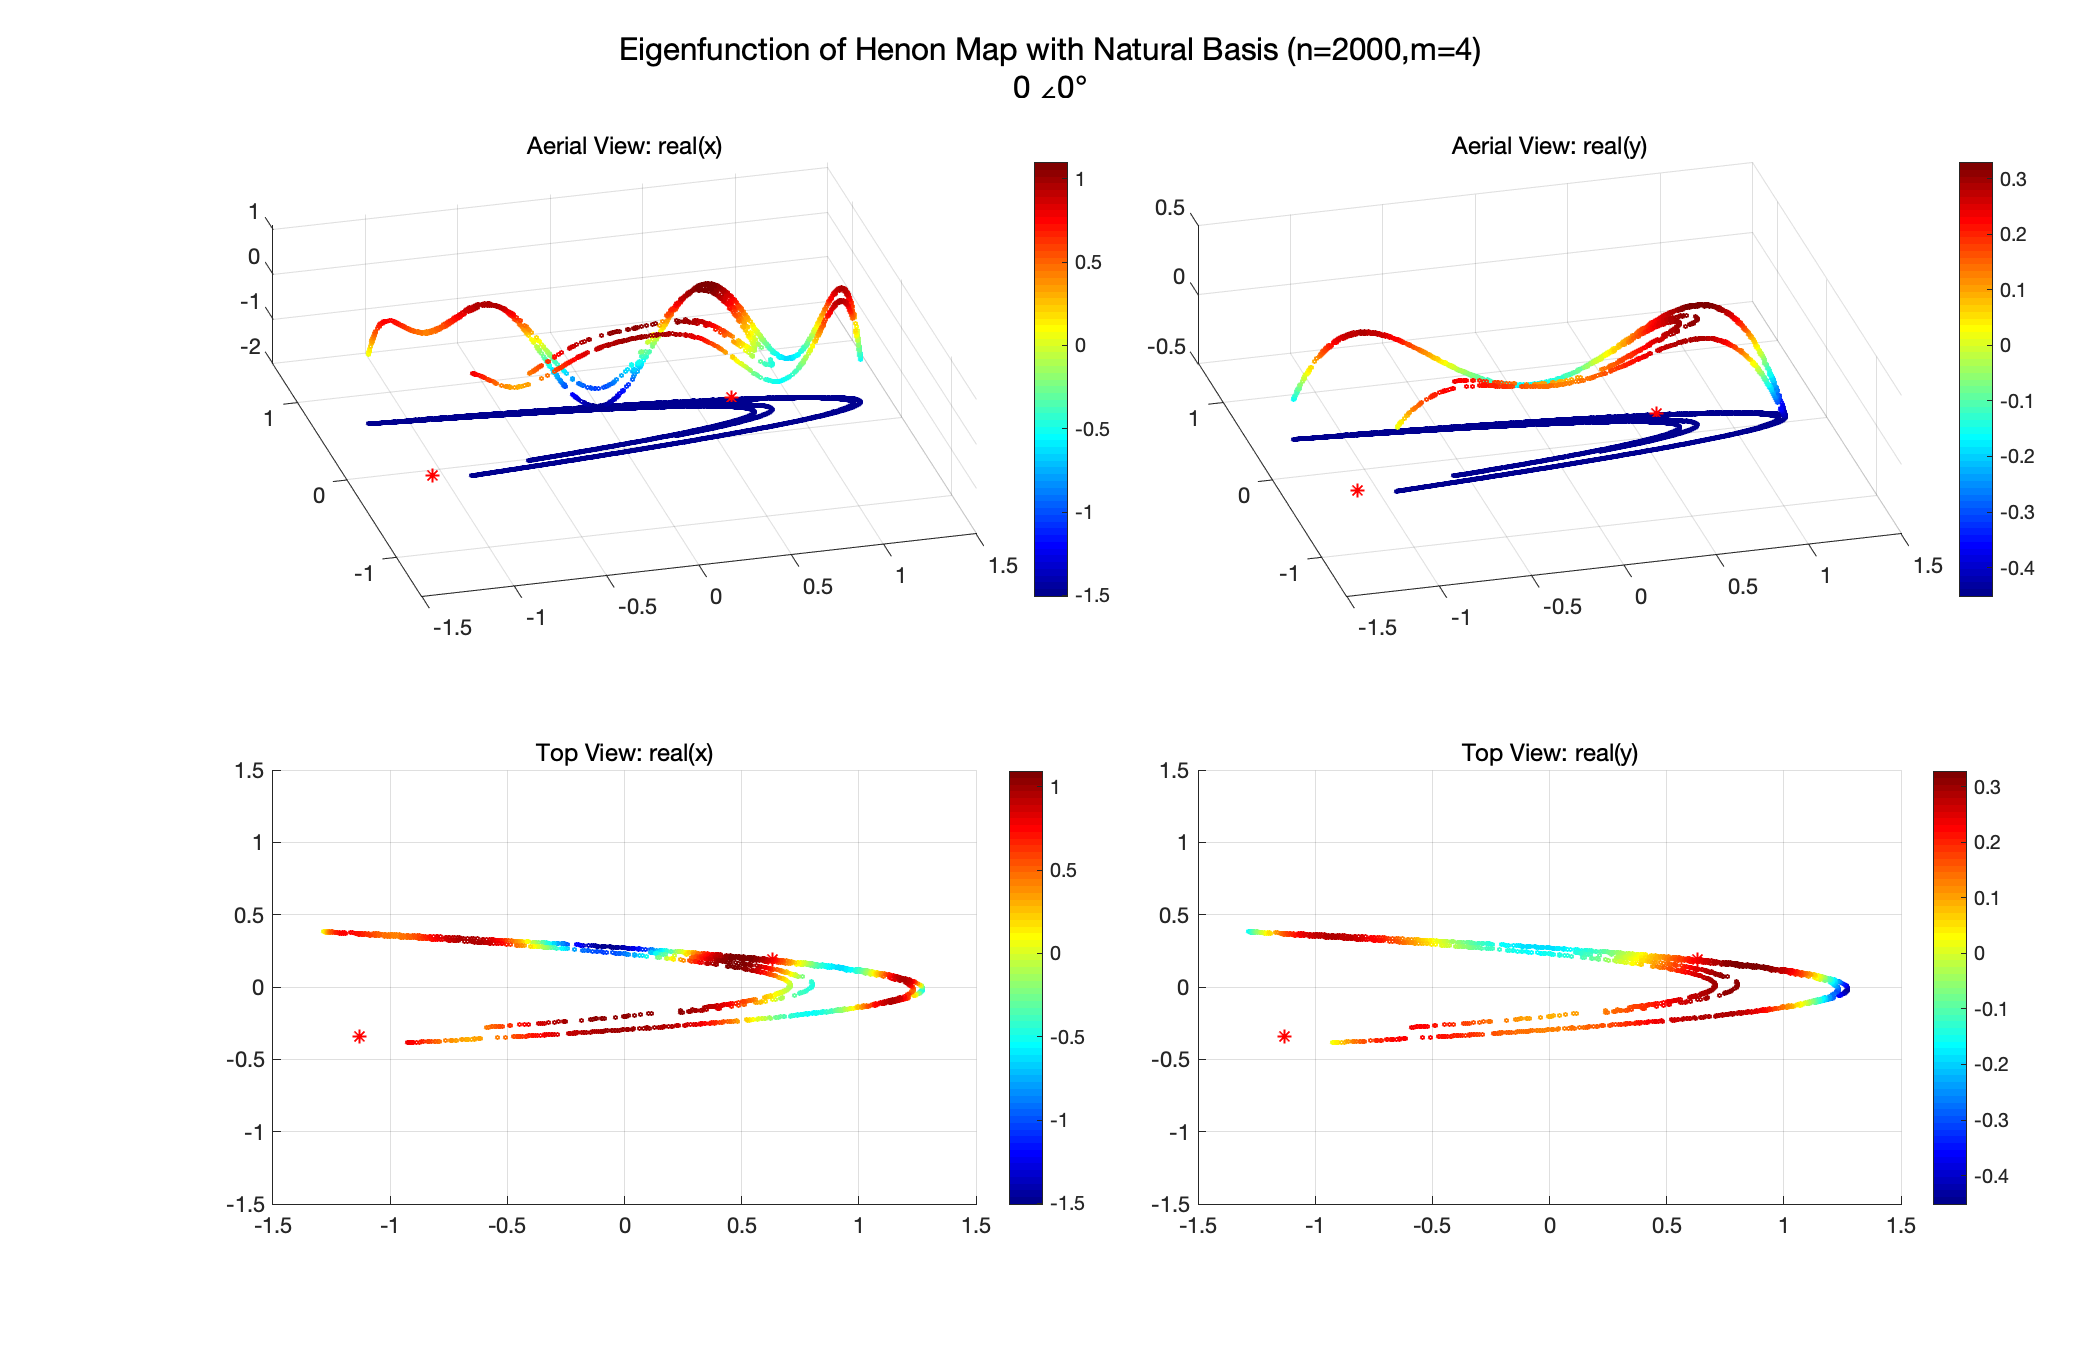
\includegraphics[scale=0.2]{henon/natural/Henon_eigen_natural_n2000m4_figure1}}
    \subfloat{
      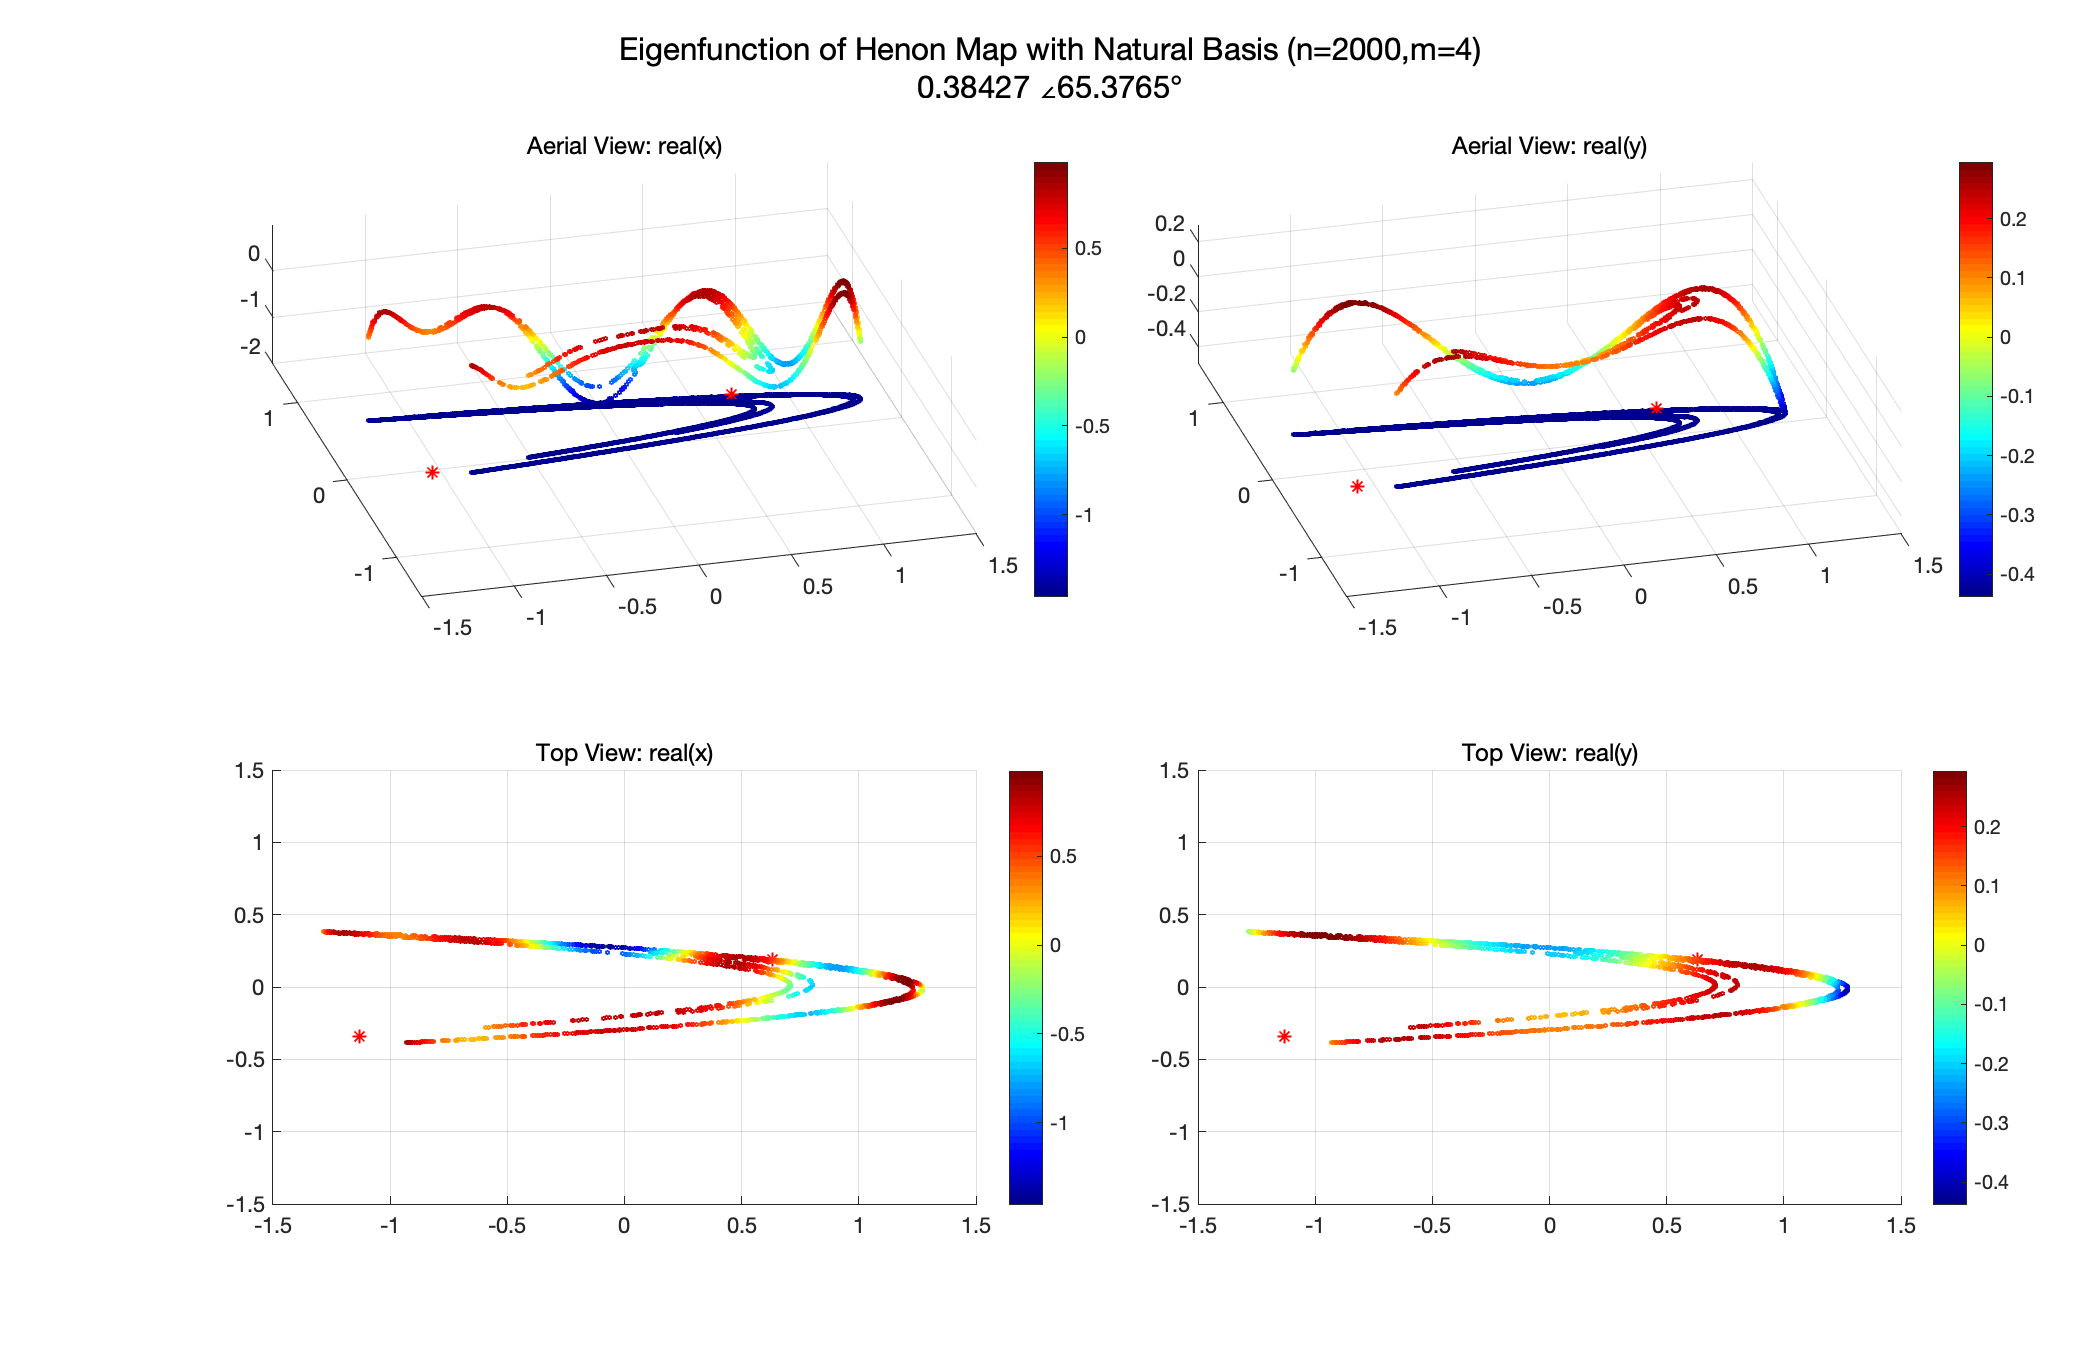
\includegraphics[scale=0.2]{henon/natural/Henon_eigen_natural_n2000m4_figure2}}
    \\
    \subfloat{
      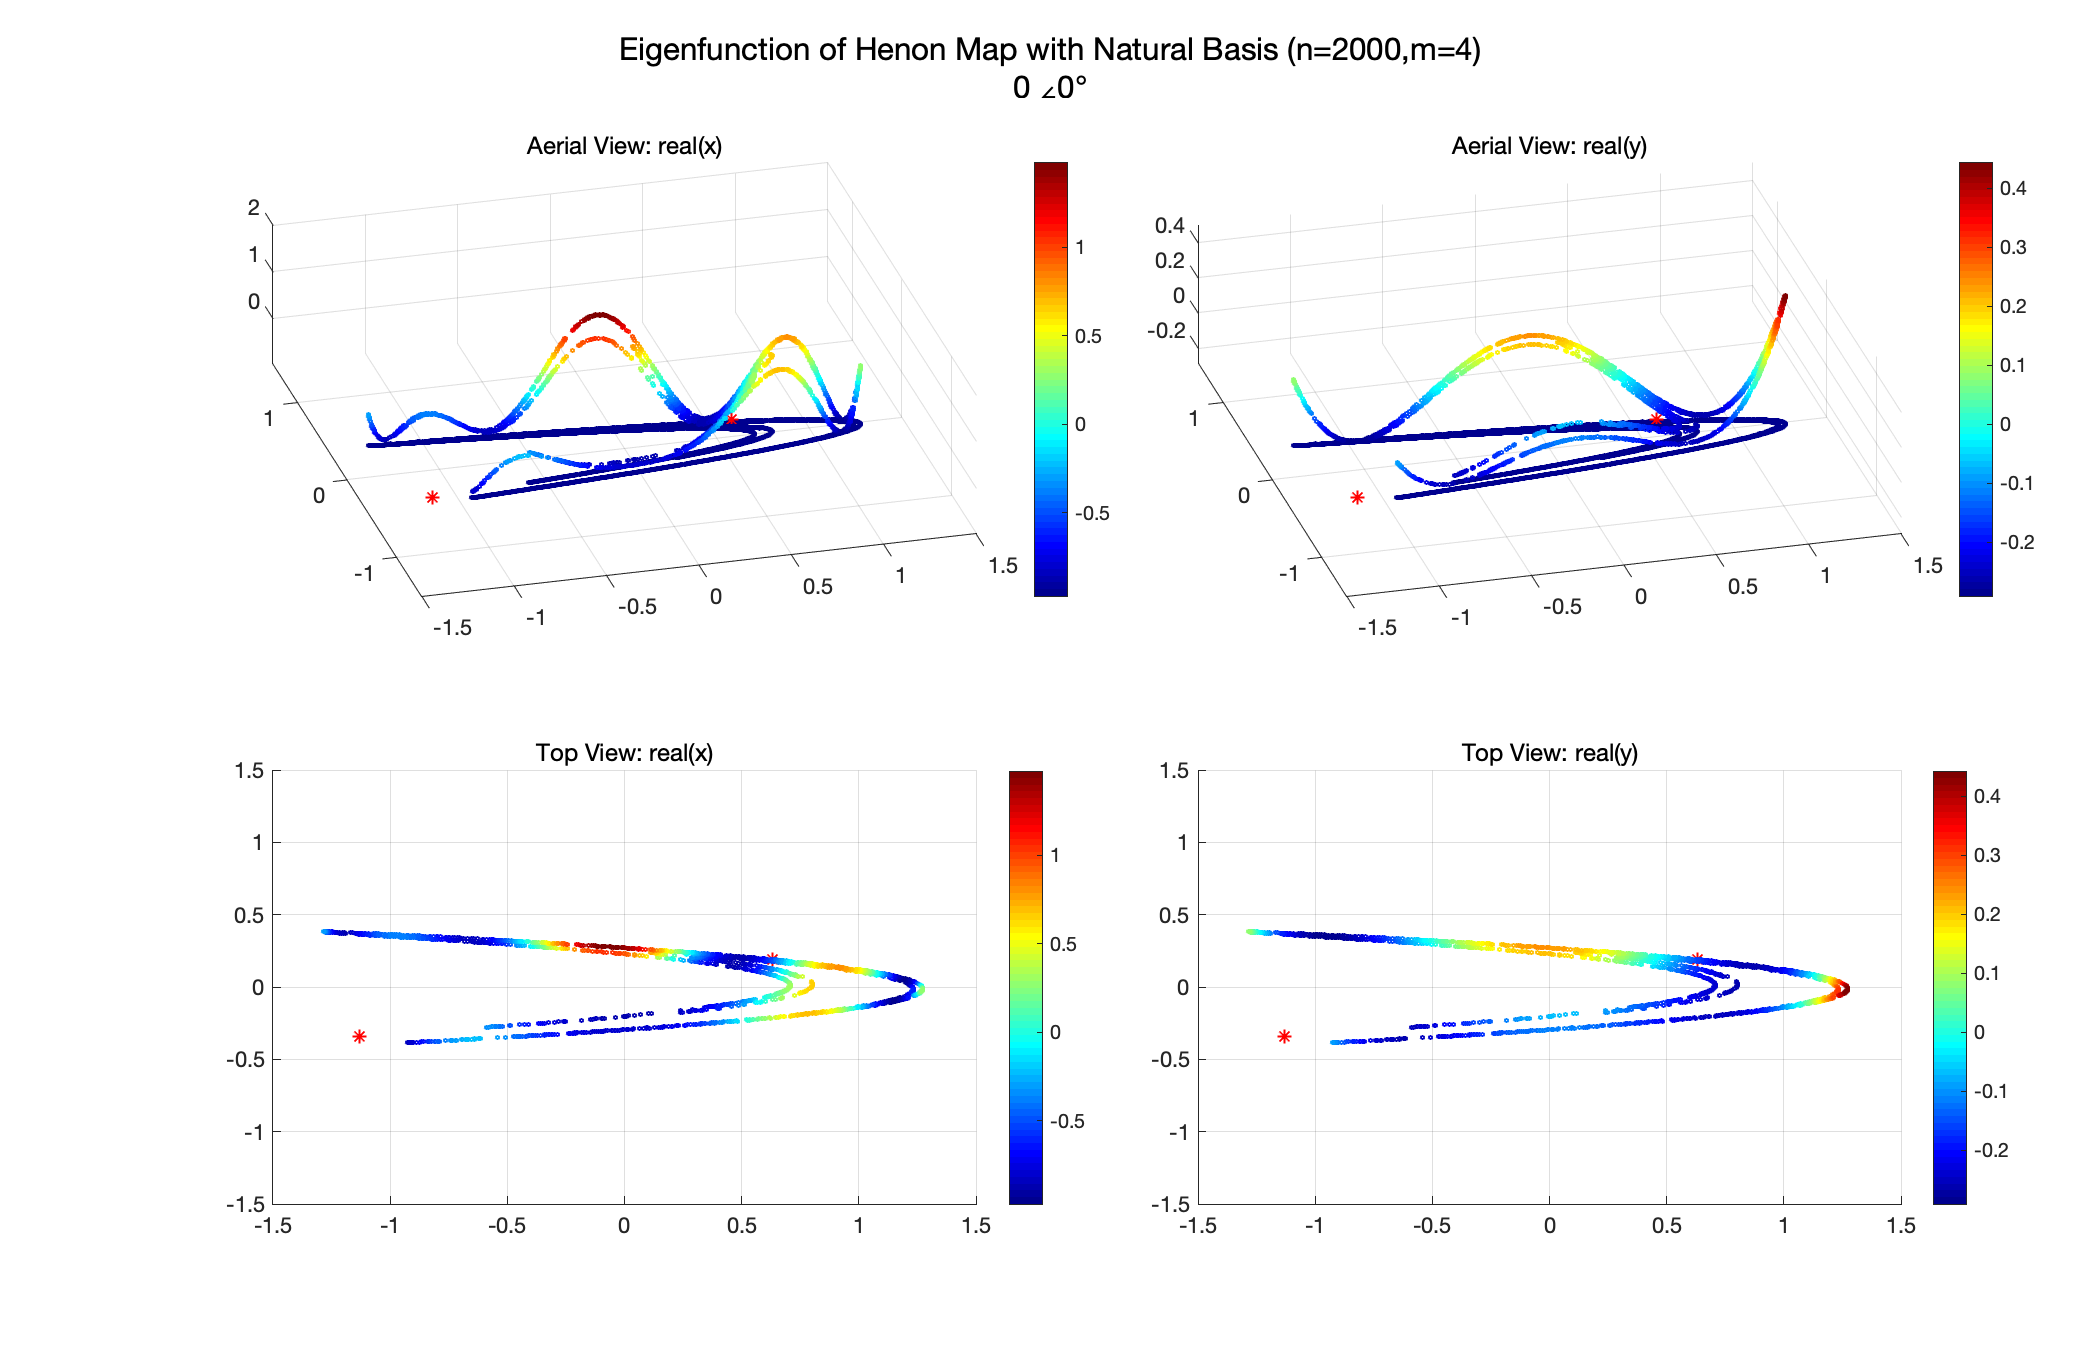
\includegraphics[scale=0.2]{henon/natural/Henon_eigen_natural_n2000m4_figure3}}
    \subfloat{
      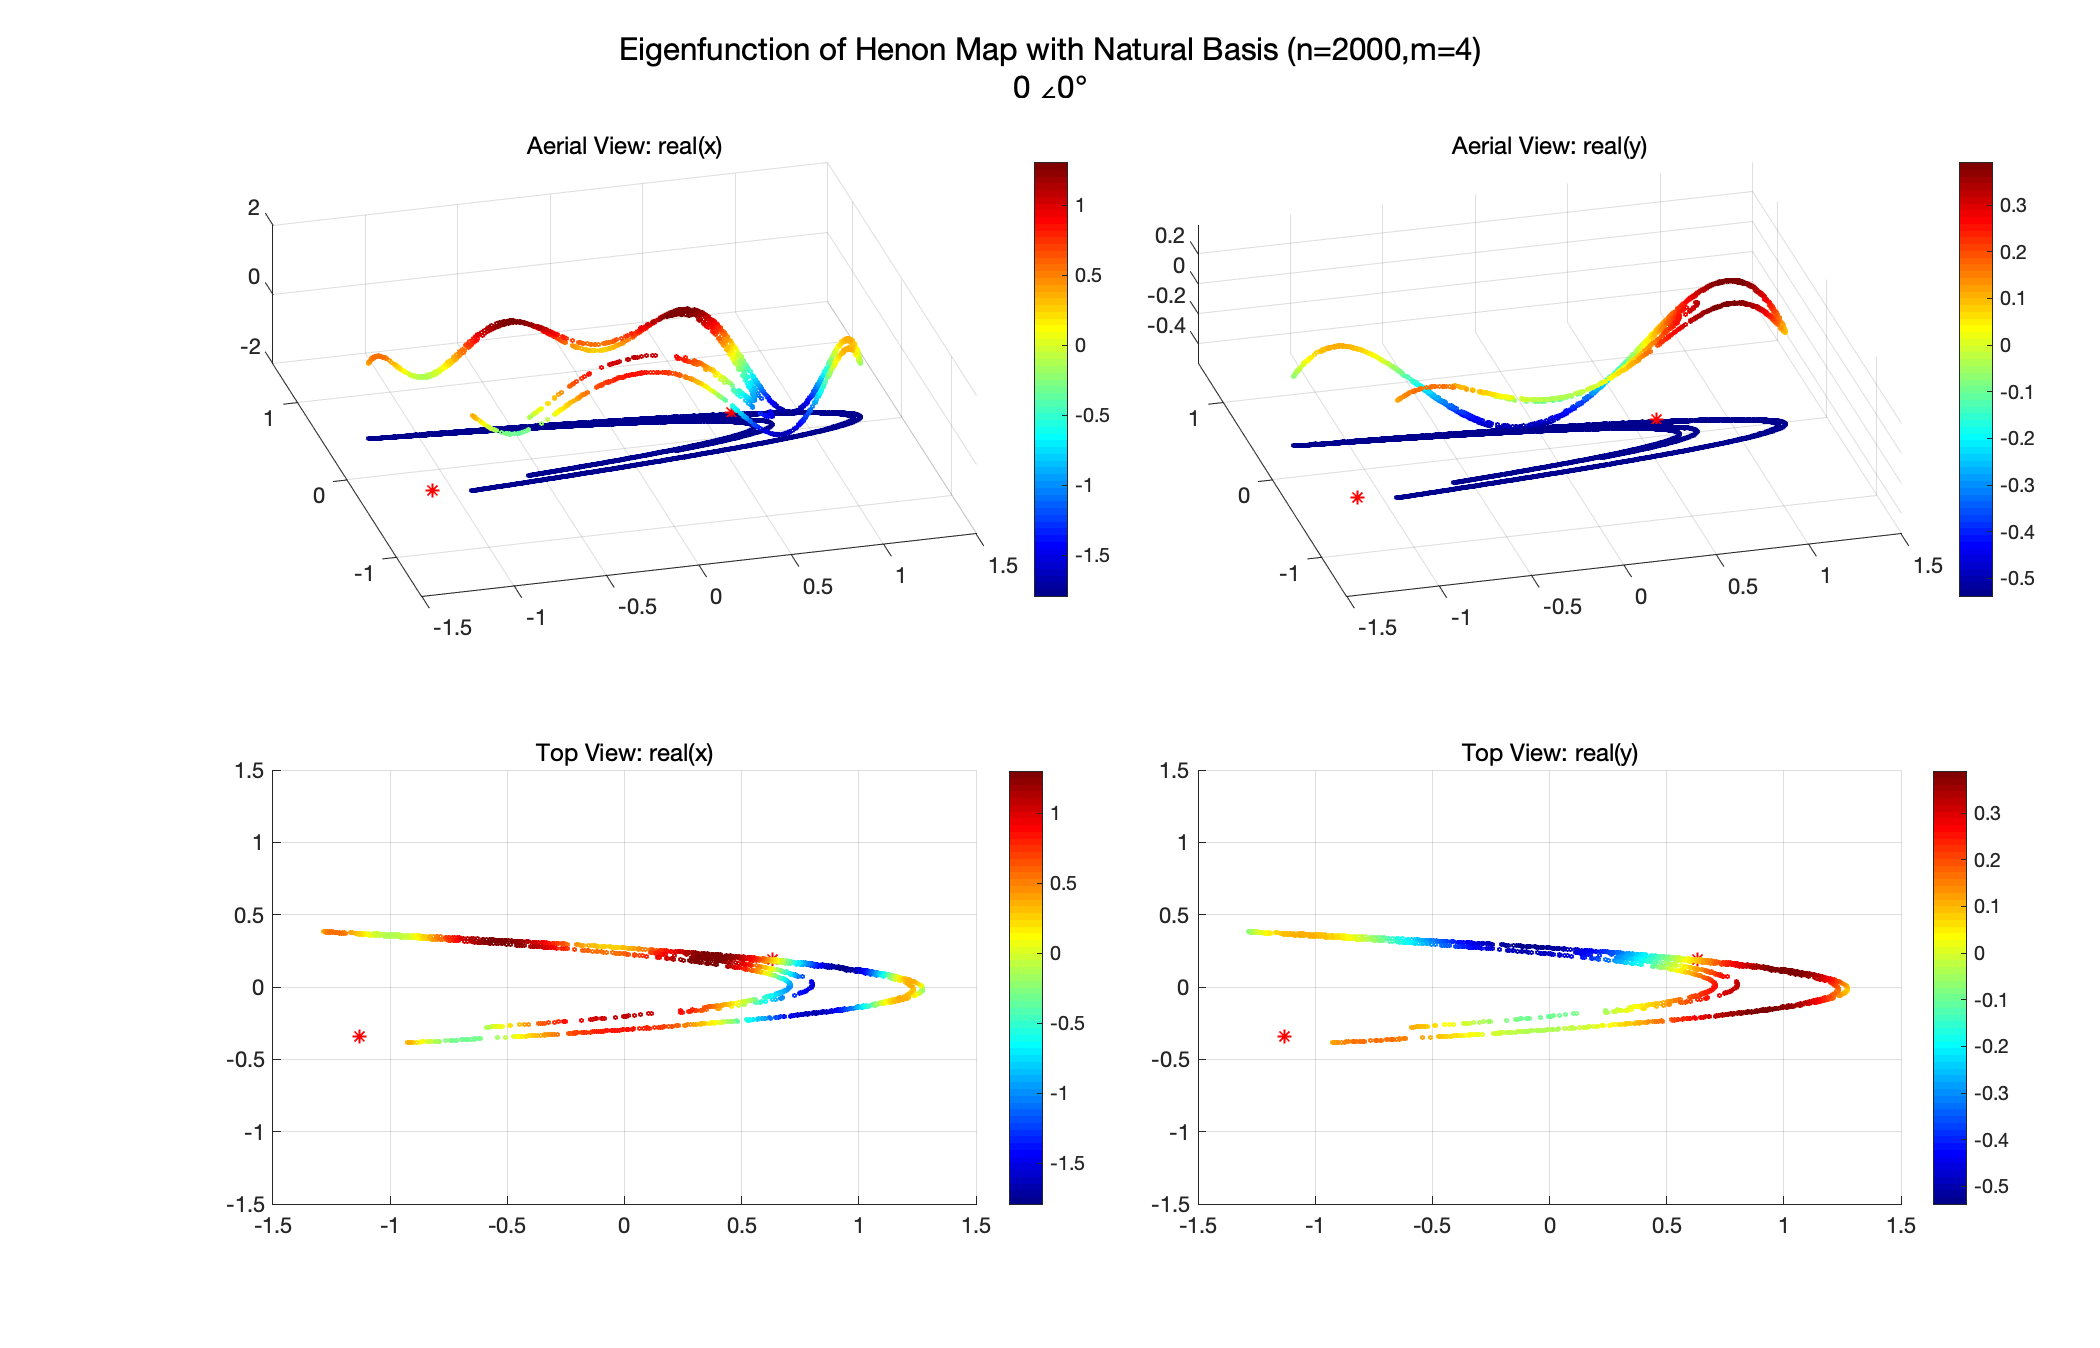
\includegraphics[scale=0.2]{henon/natural/Henon_eigen_natural_n2000m4_figure4}}
    \\
    \caption{埃农映射自然基函数下的本征函数($n=2000$,$m=4$)}
\end{figure}

\begin{figure}
    \centering
    \subfloat[m=1]{
      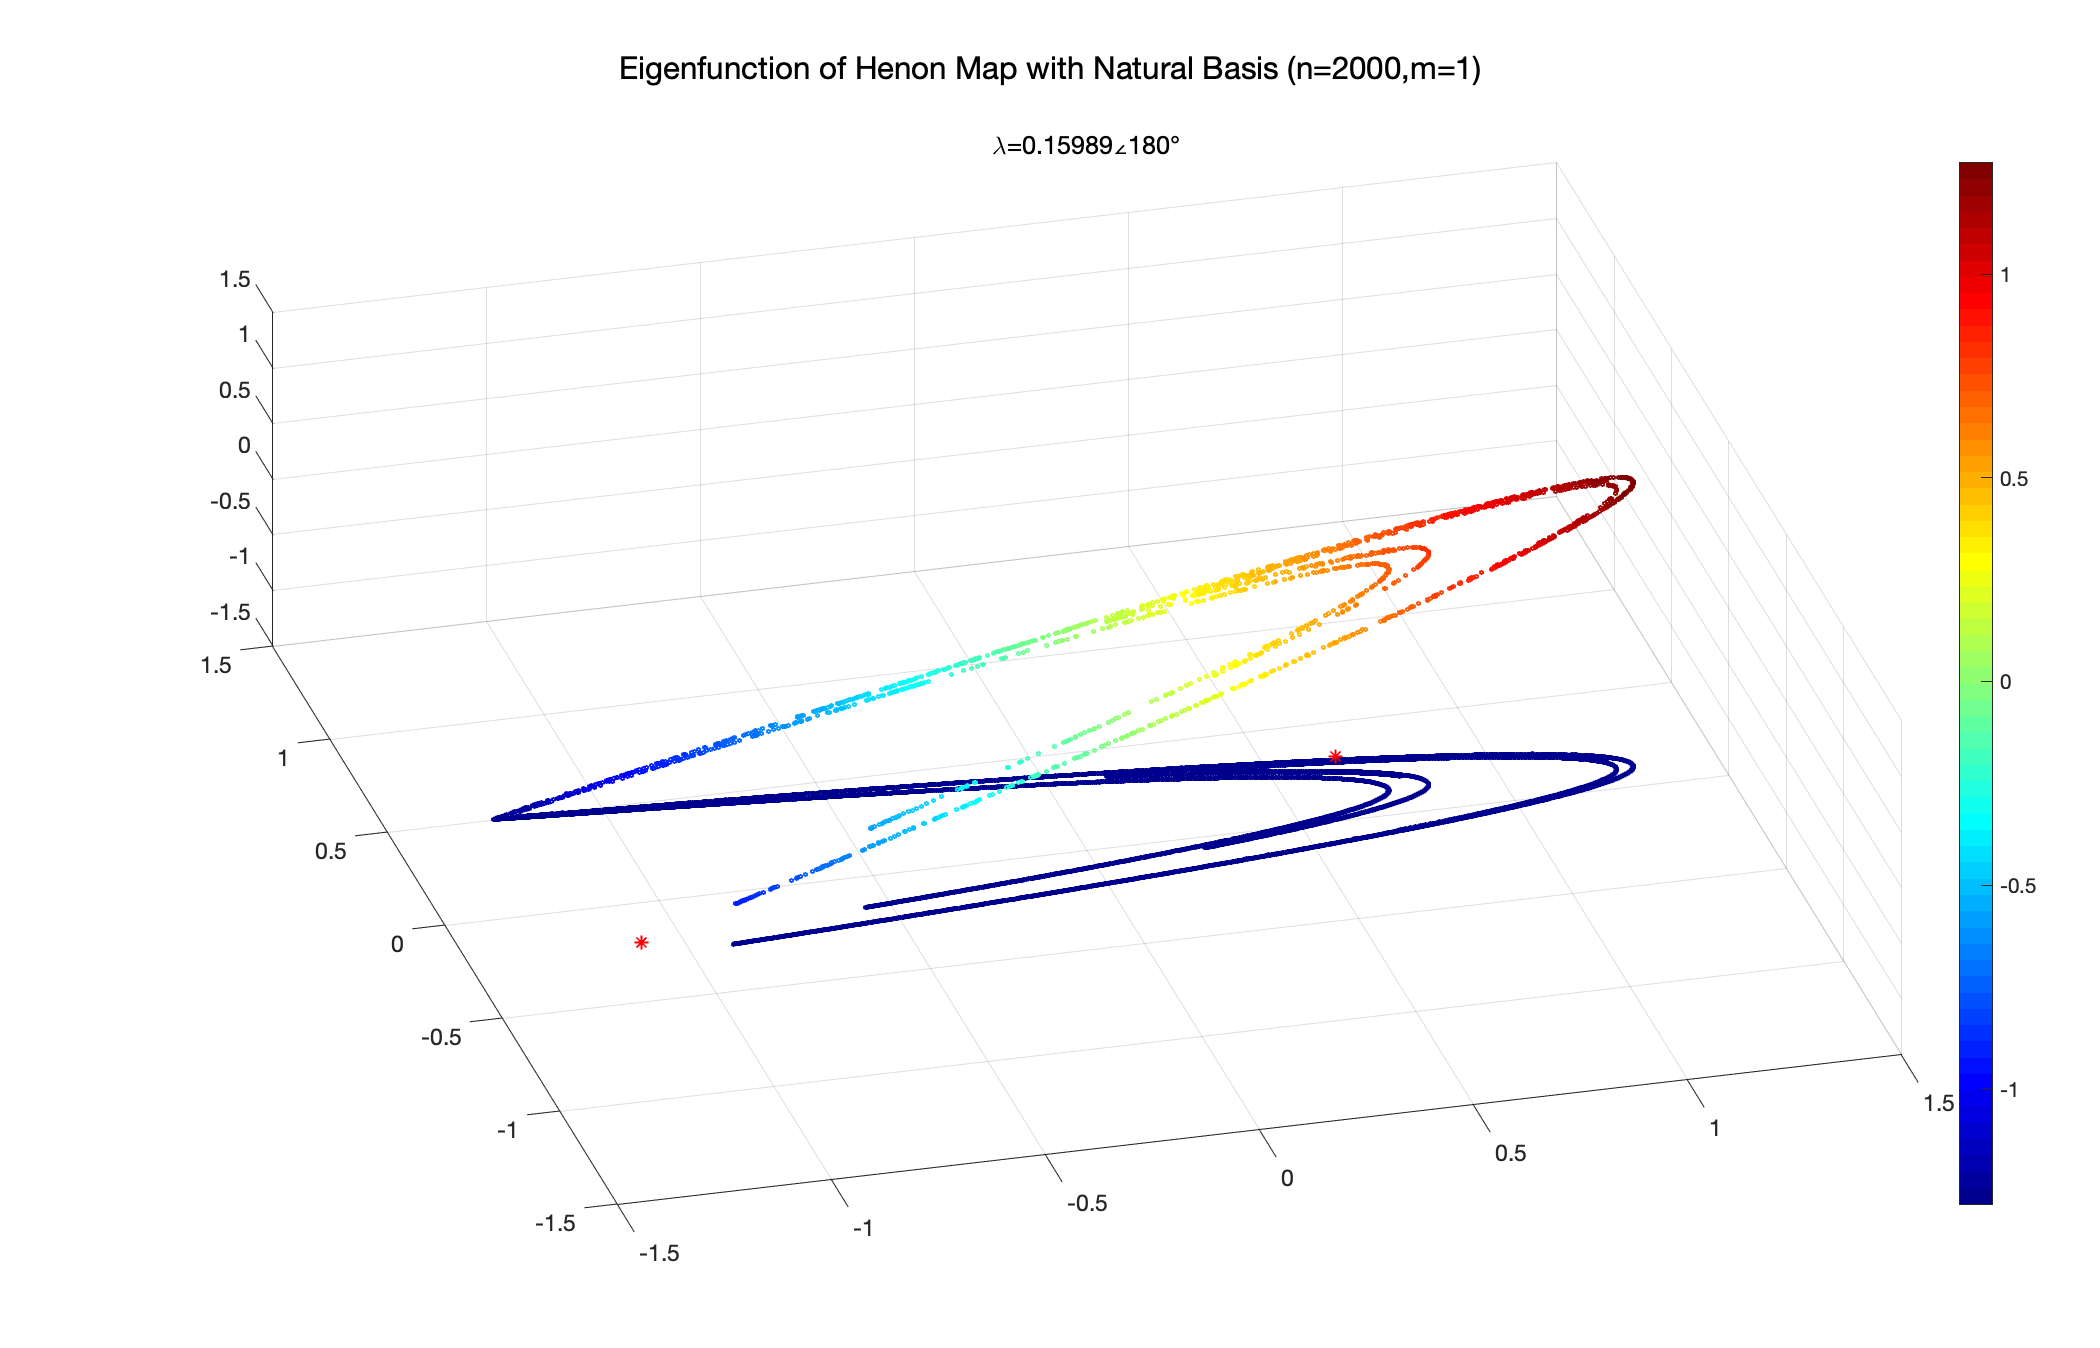
\includegraphics[scale=0.2]{henon/natural/Henon_eigen_natural_n2000m1}}
    \subfloat[m=2]{
      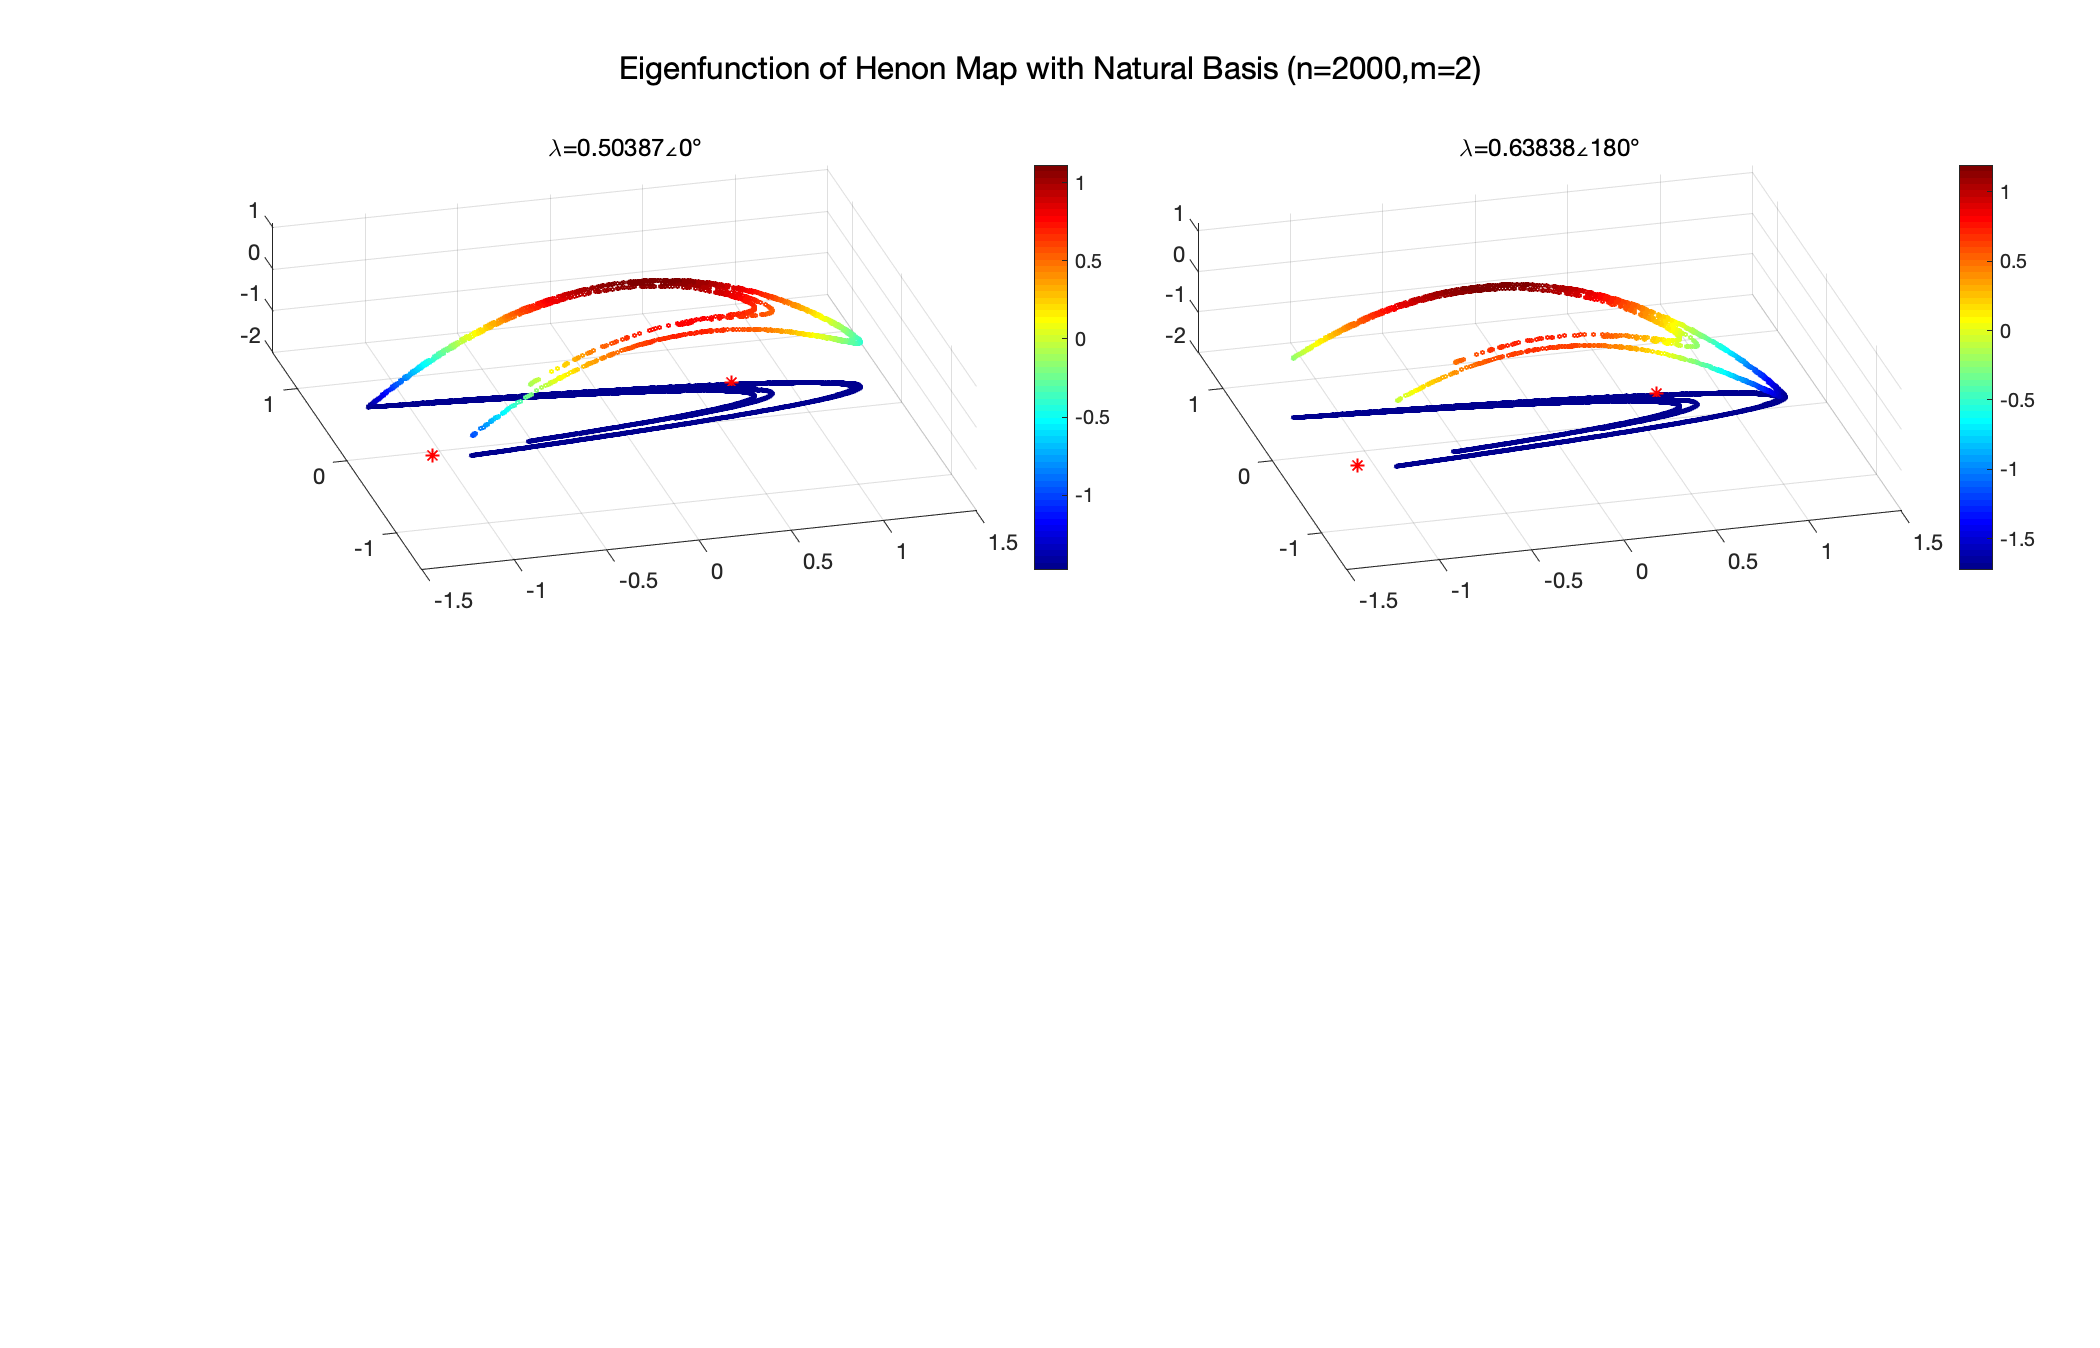
\includegraphics[scale=0.2]{henon/natural/Henon_eigen_natural_n2000m2}}
    \\
    \subfloat[m=3]{
      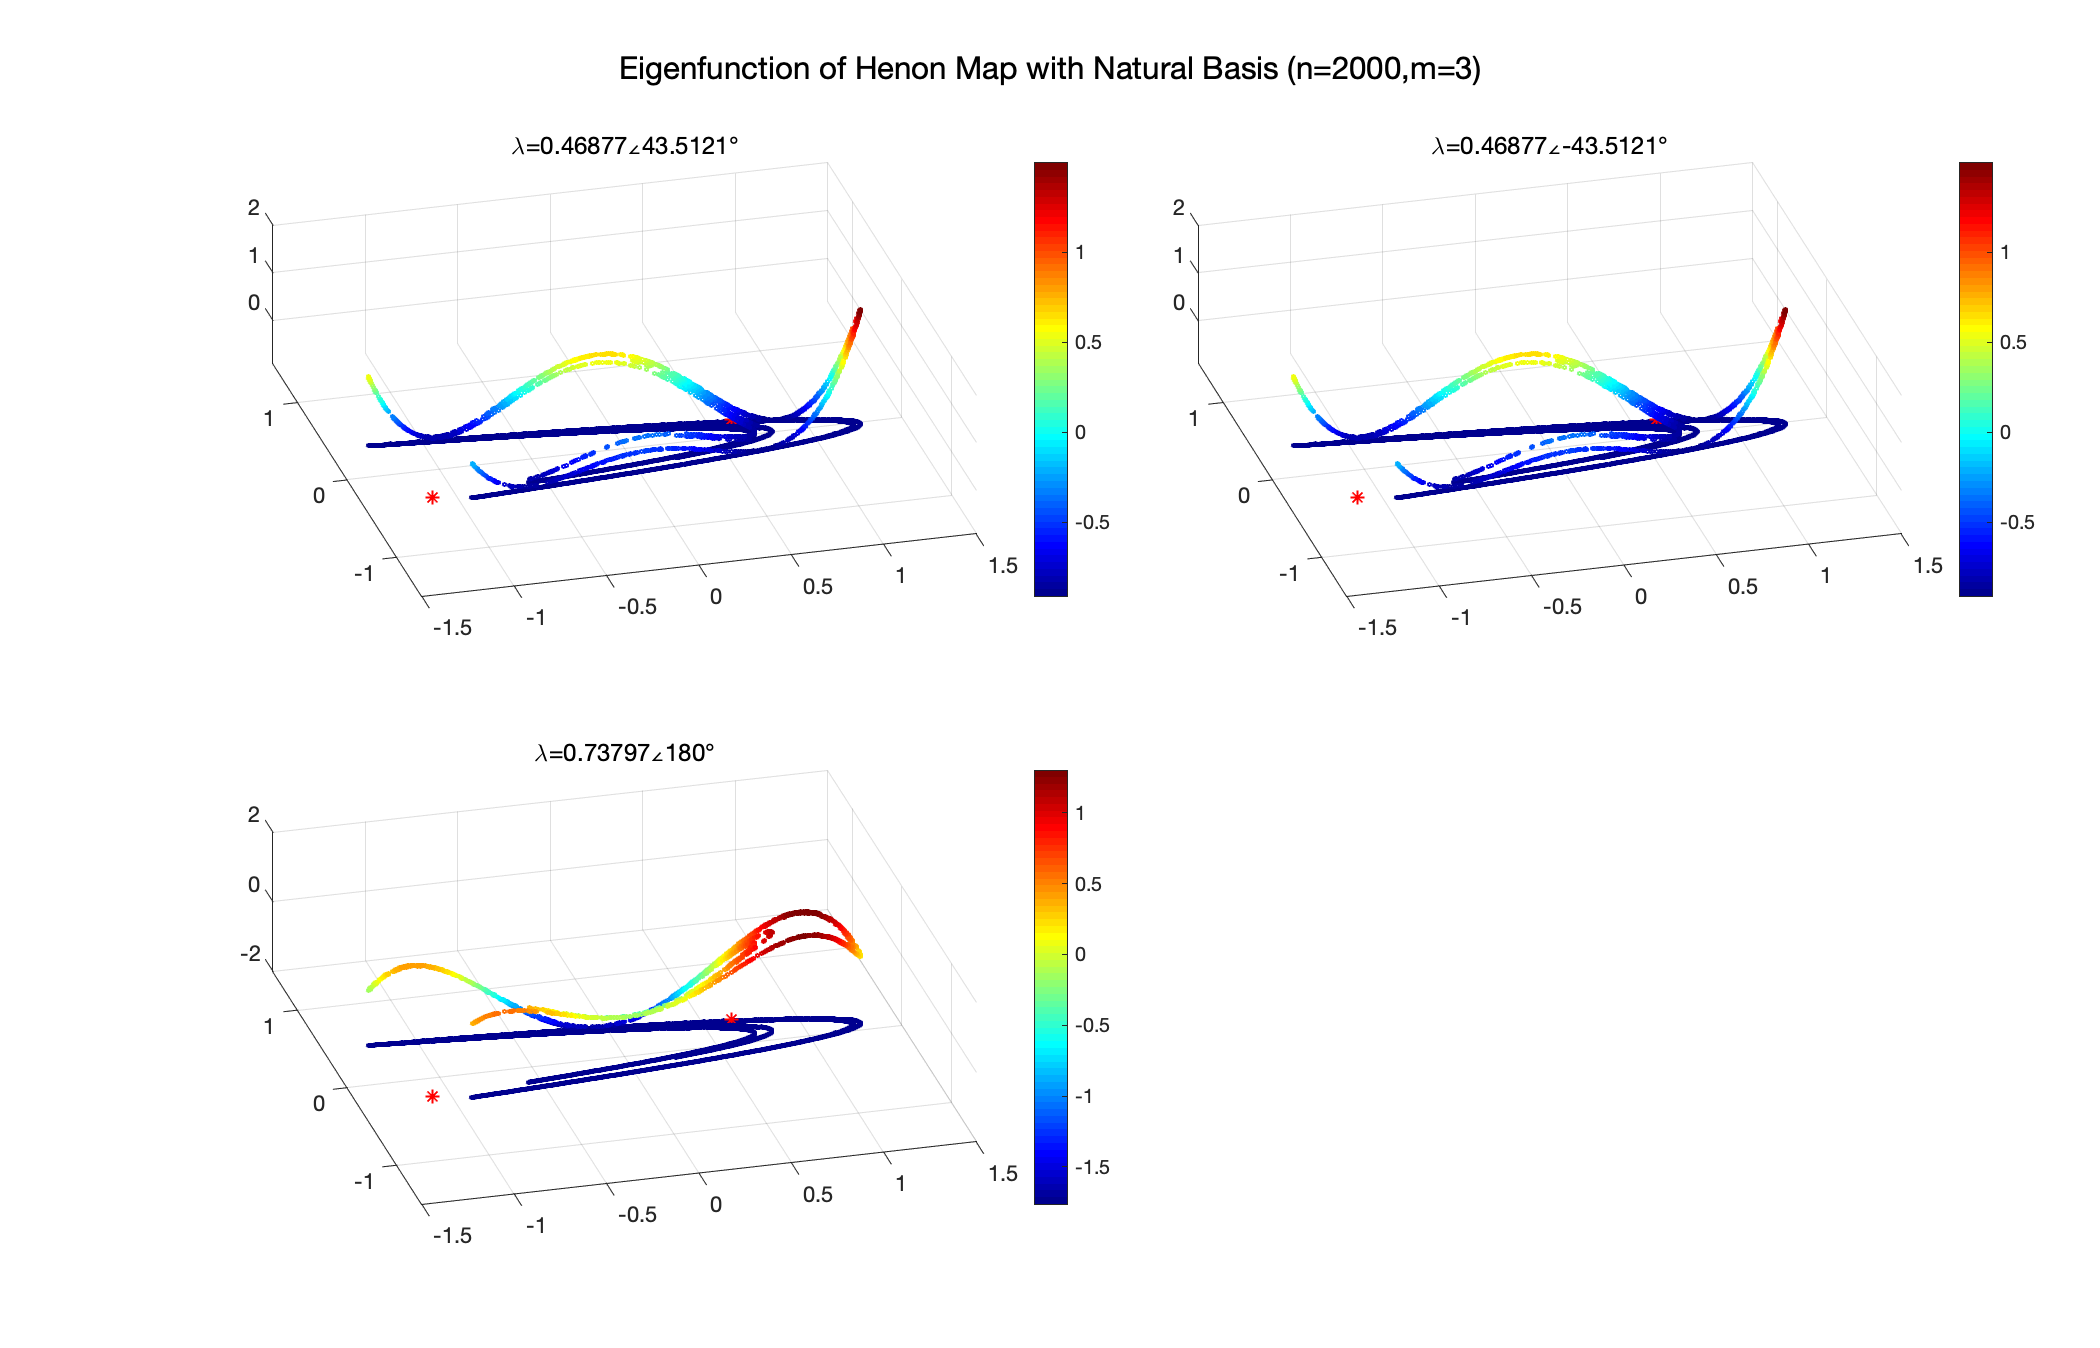
\includegraphics[scale=0.2]{henon/natural/Henon_eigen_natural_n2000m3}}
    \subfloat[m=4]{
      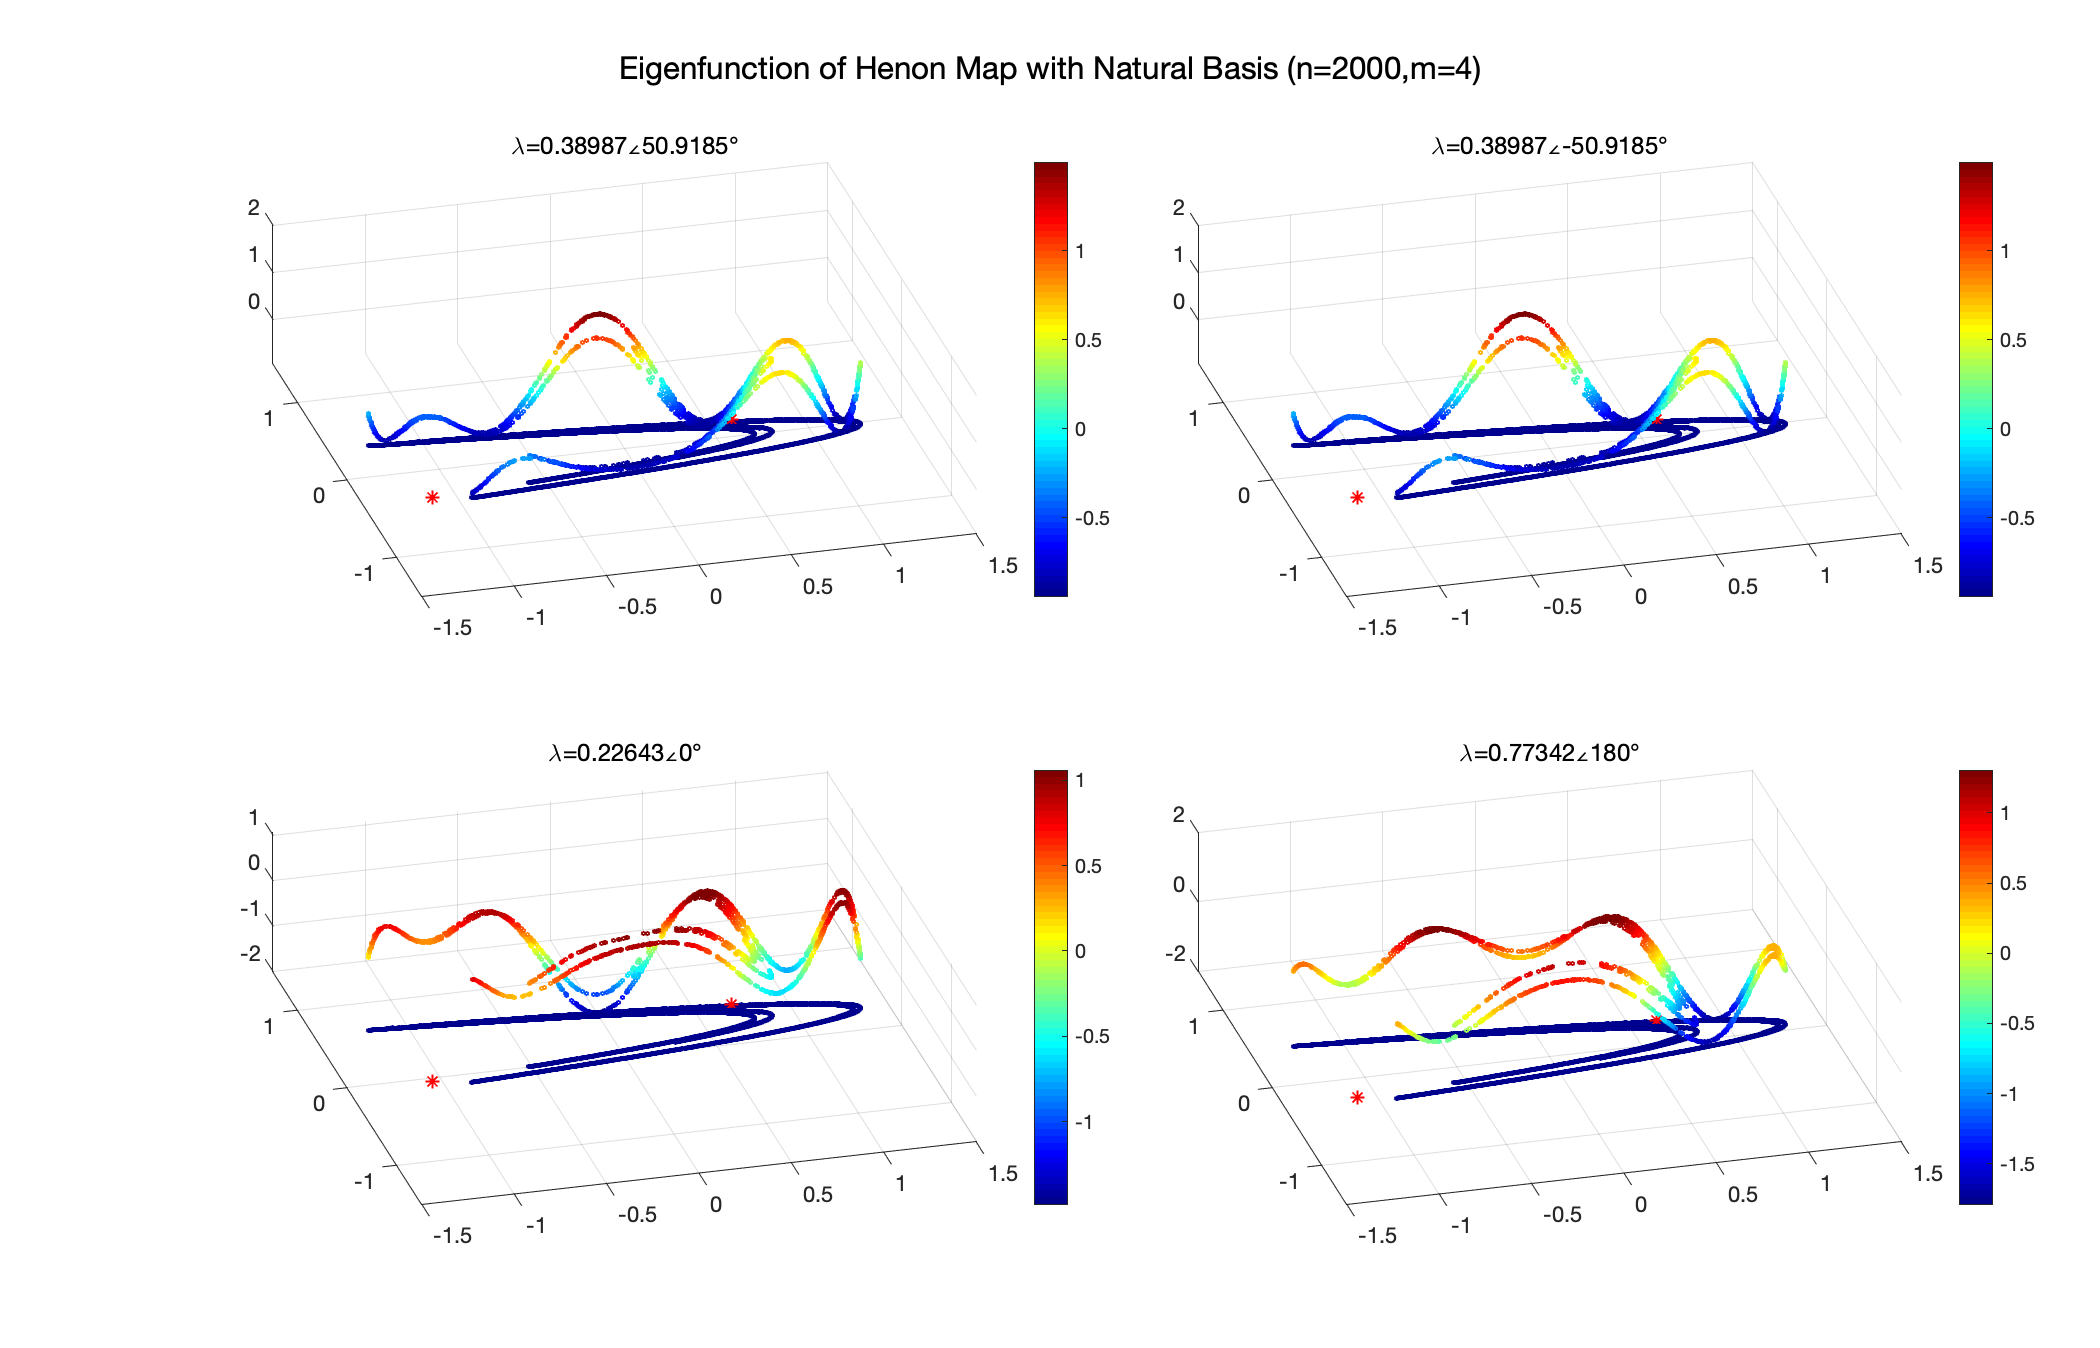
\includegraphics[scale=0.2]{henon/natural/Henon_eigen_natural_n2000m4}}
    \\
    \subfloat[m=5]{
      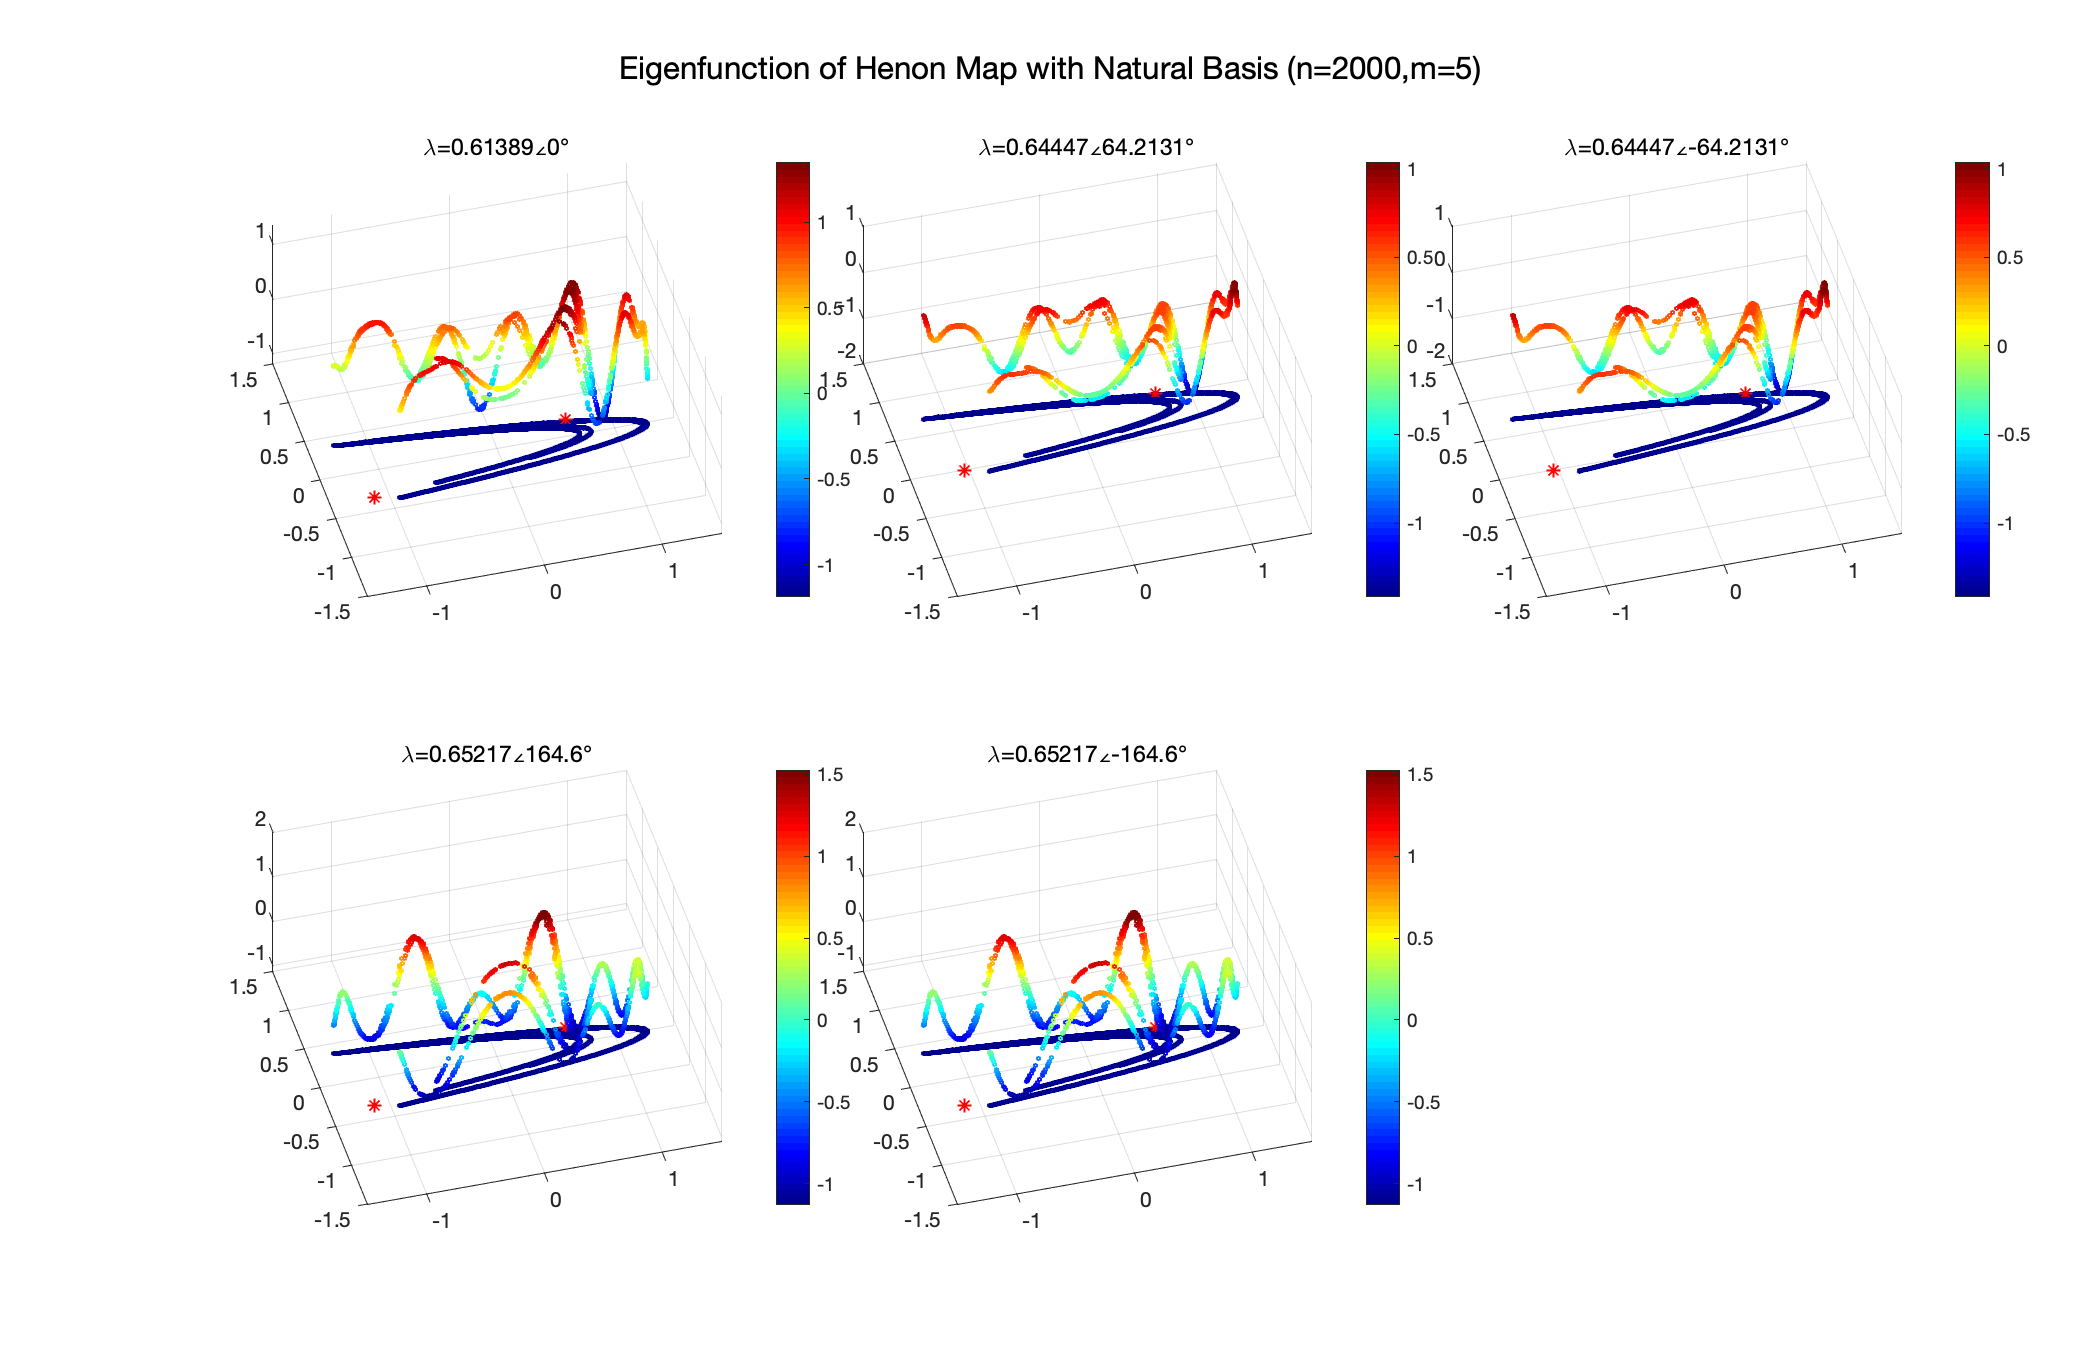
\includegraphics[scale=0.2]{henon/natural/Henon_eigen_natural_n2000m5}}
    \subfloat[m=6]{
      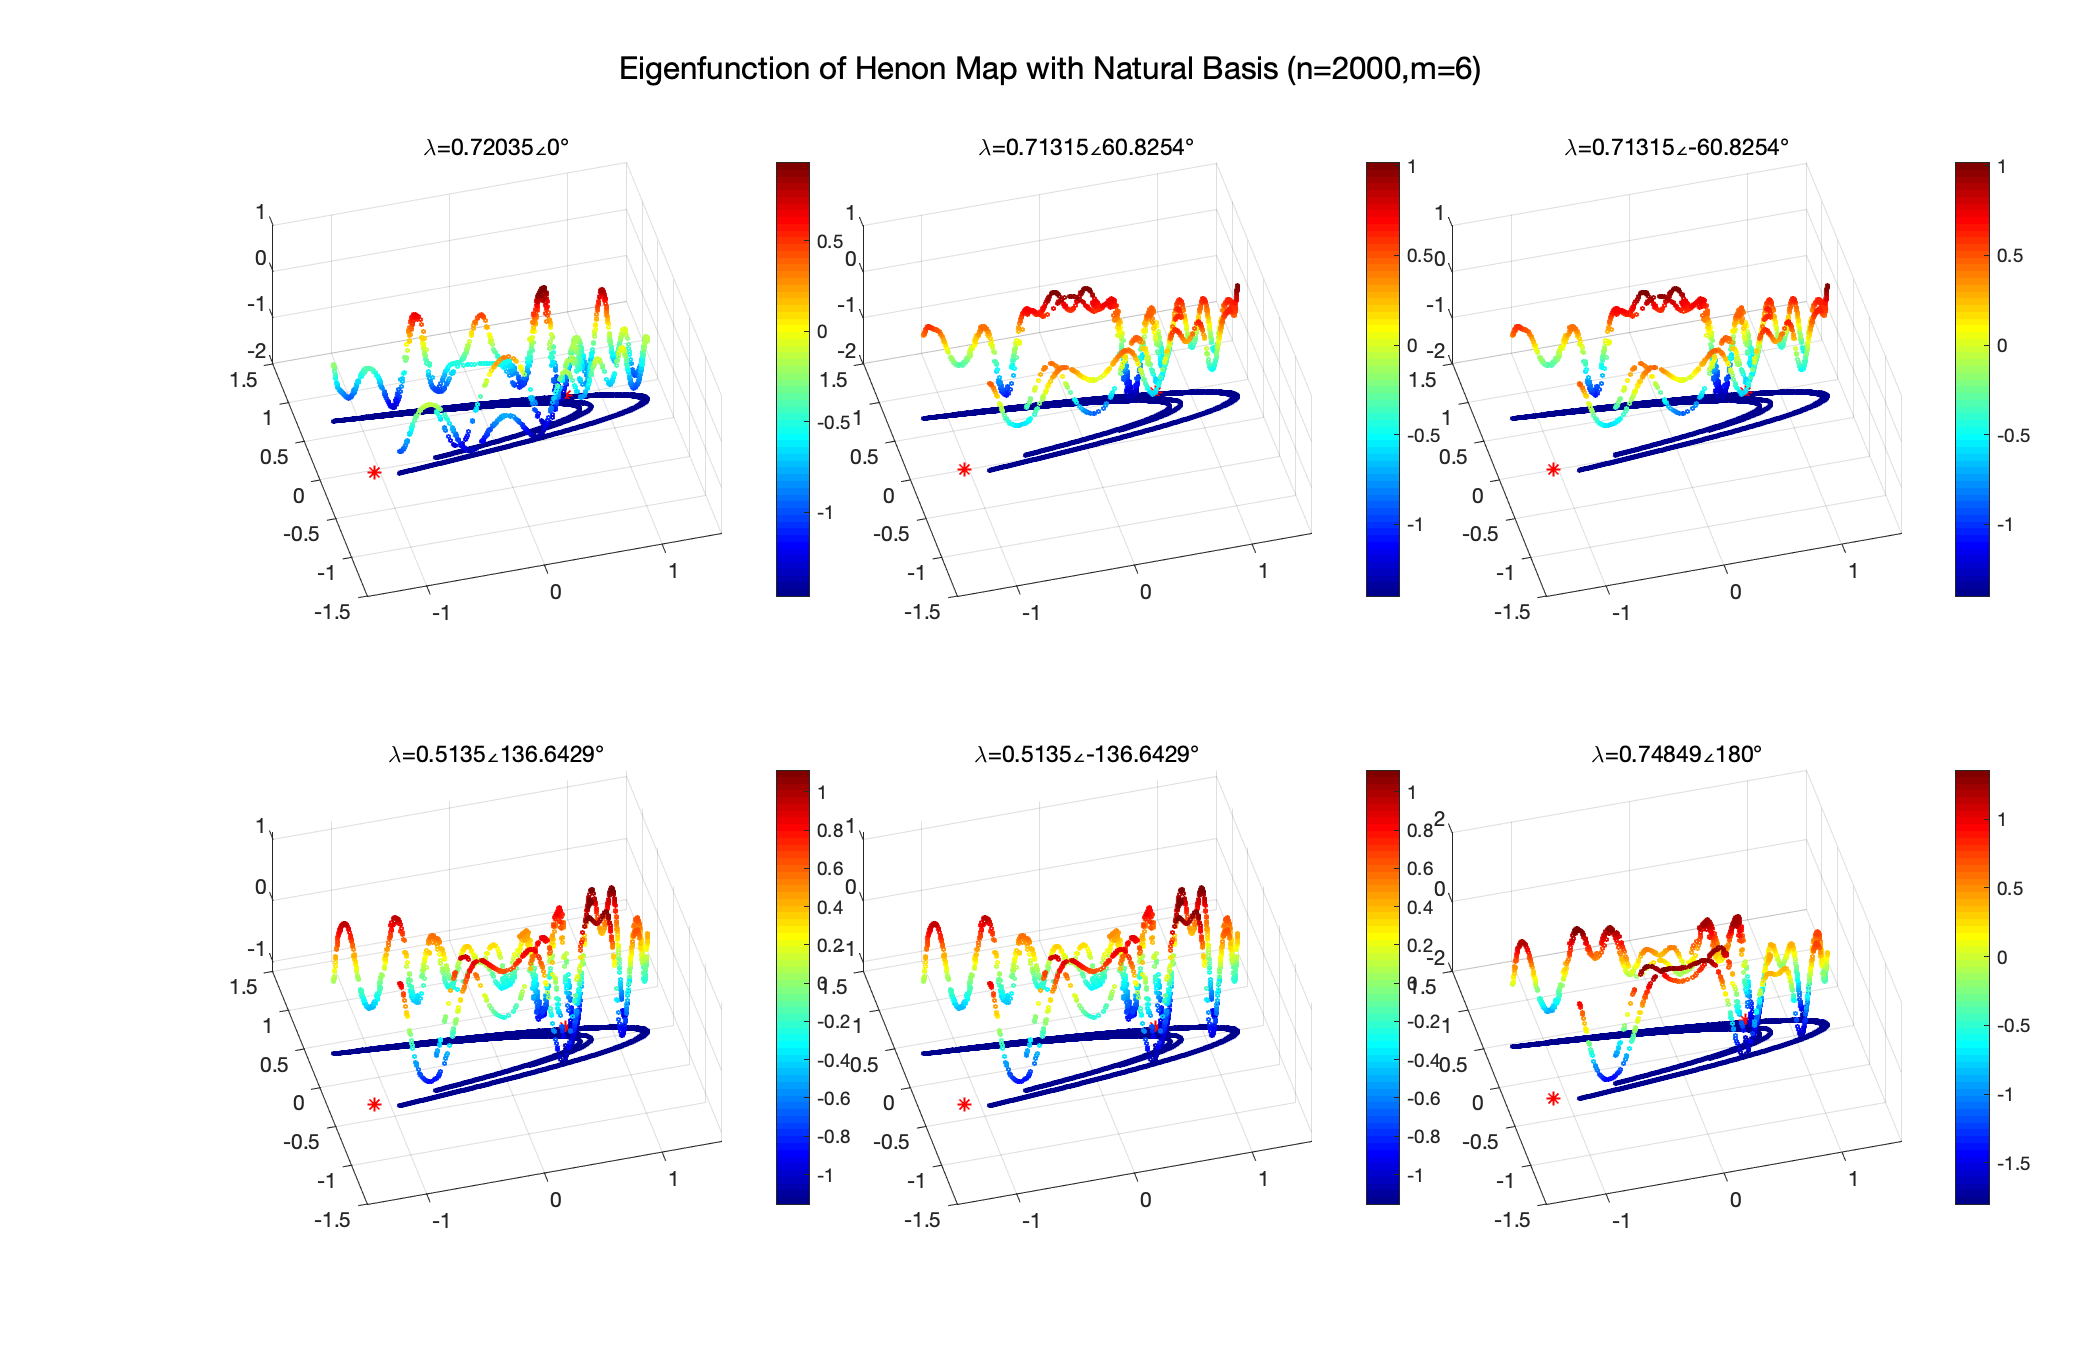
\includegraphics[scale=0.2]{henon/natural/Henon_eigen_natural_n2000m6}}
    \\
    \subfloat[m=7]{
      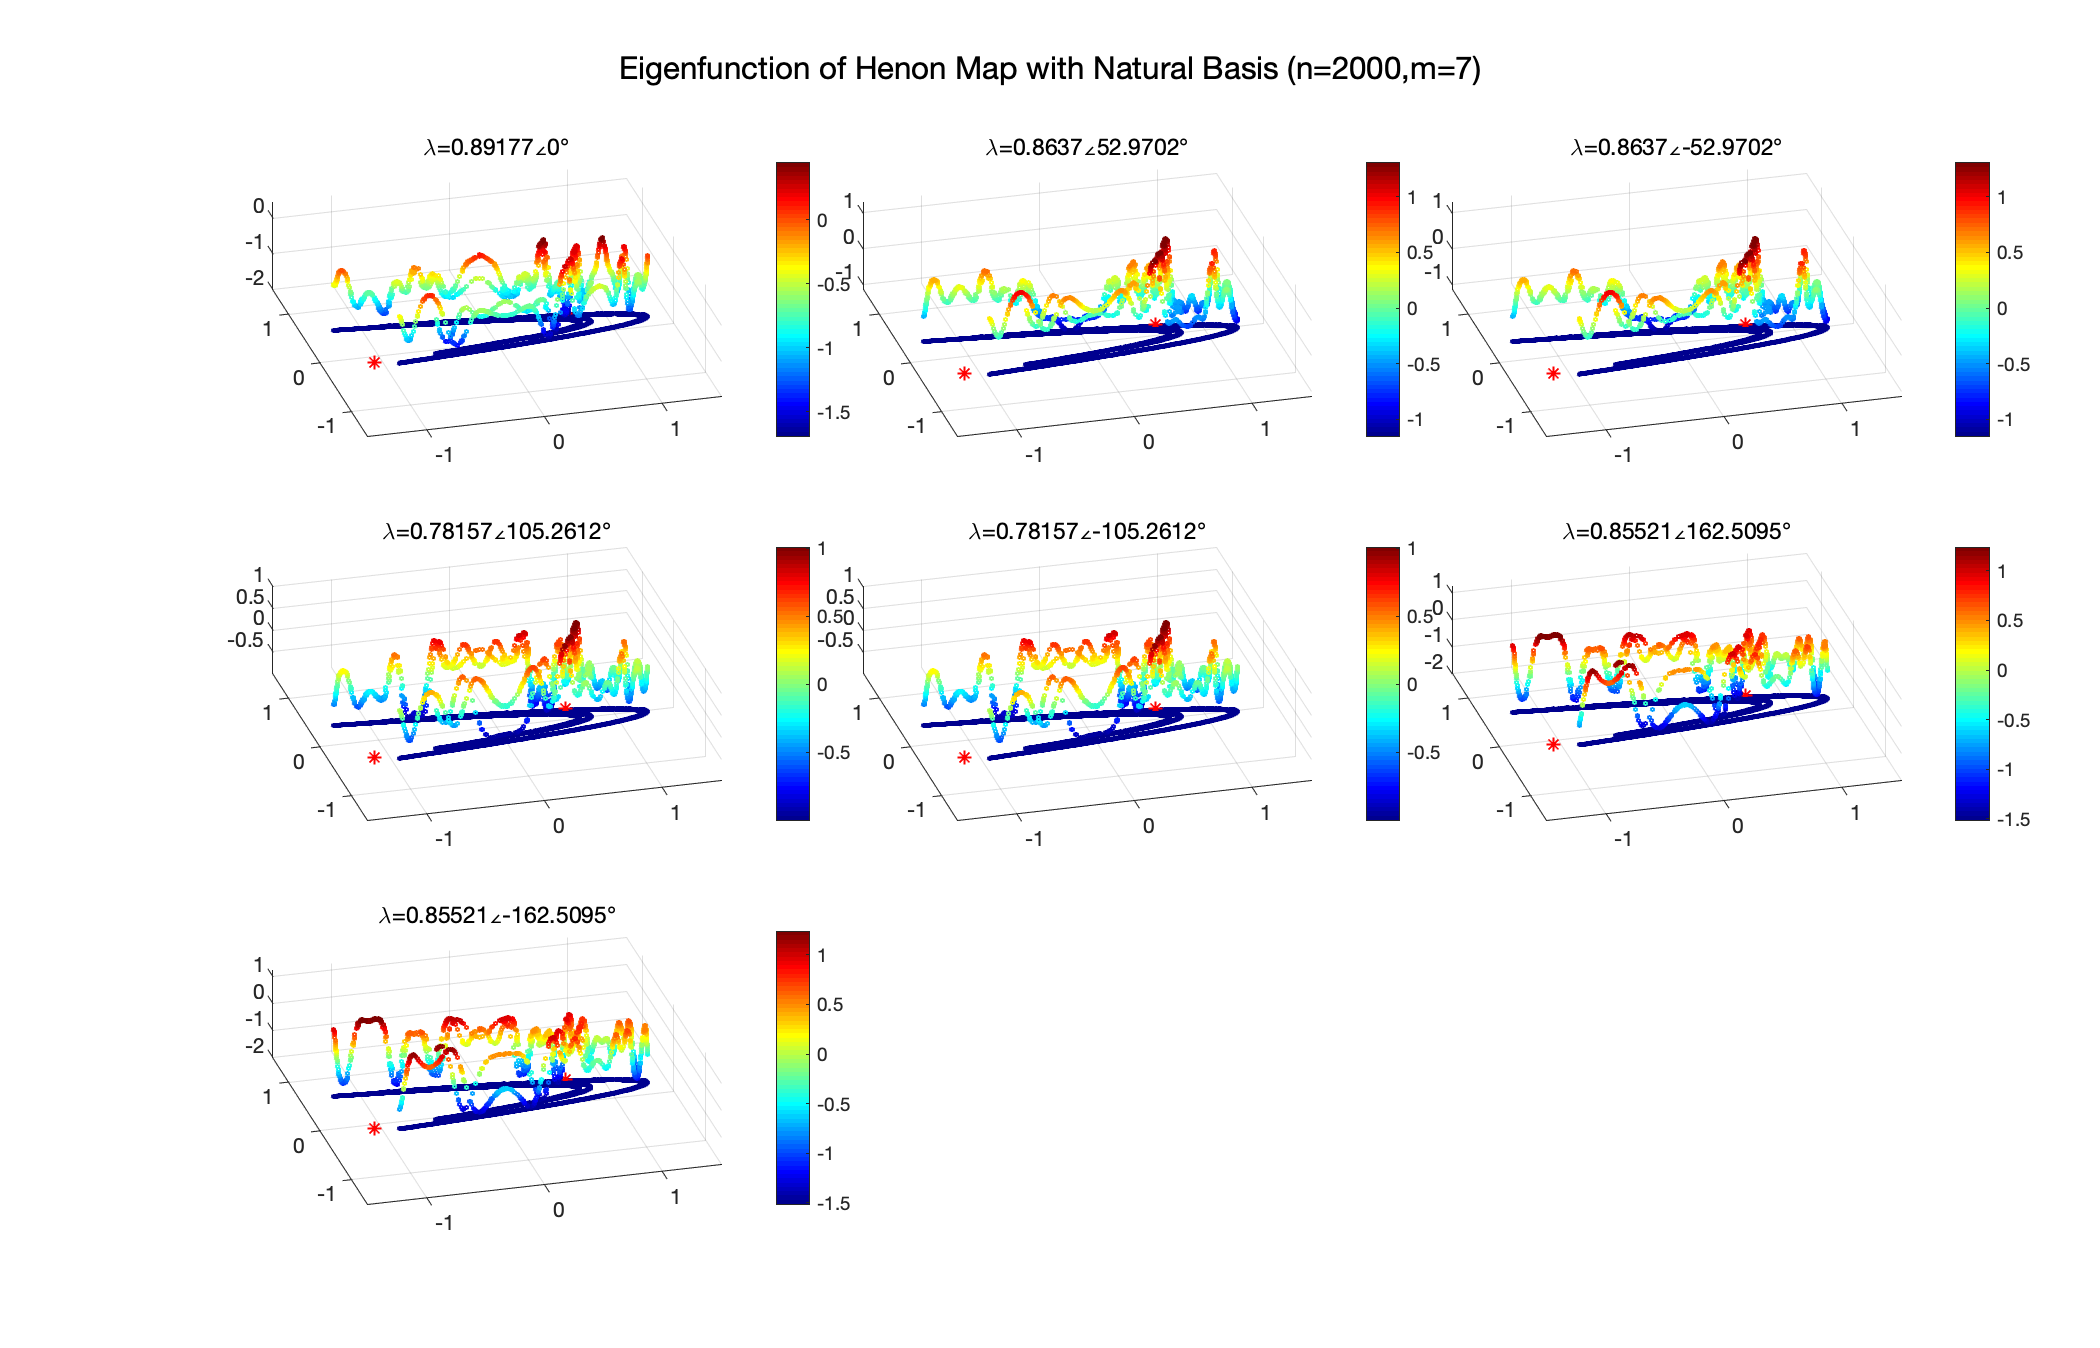
\includegraphics[scale=0.2]{henon/natural/Henon_eigen_natural_n2000m7}}
    \subfloat[m=8]{
      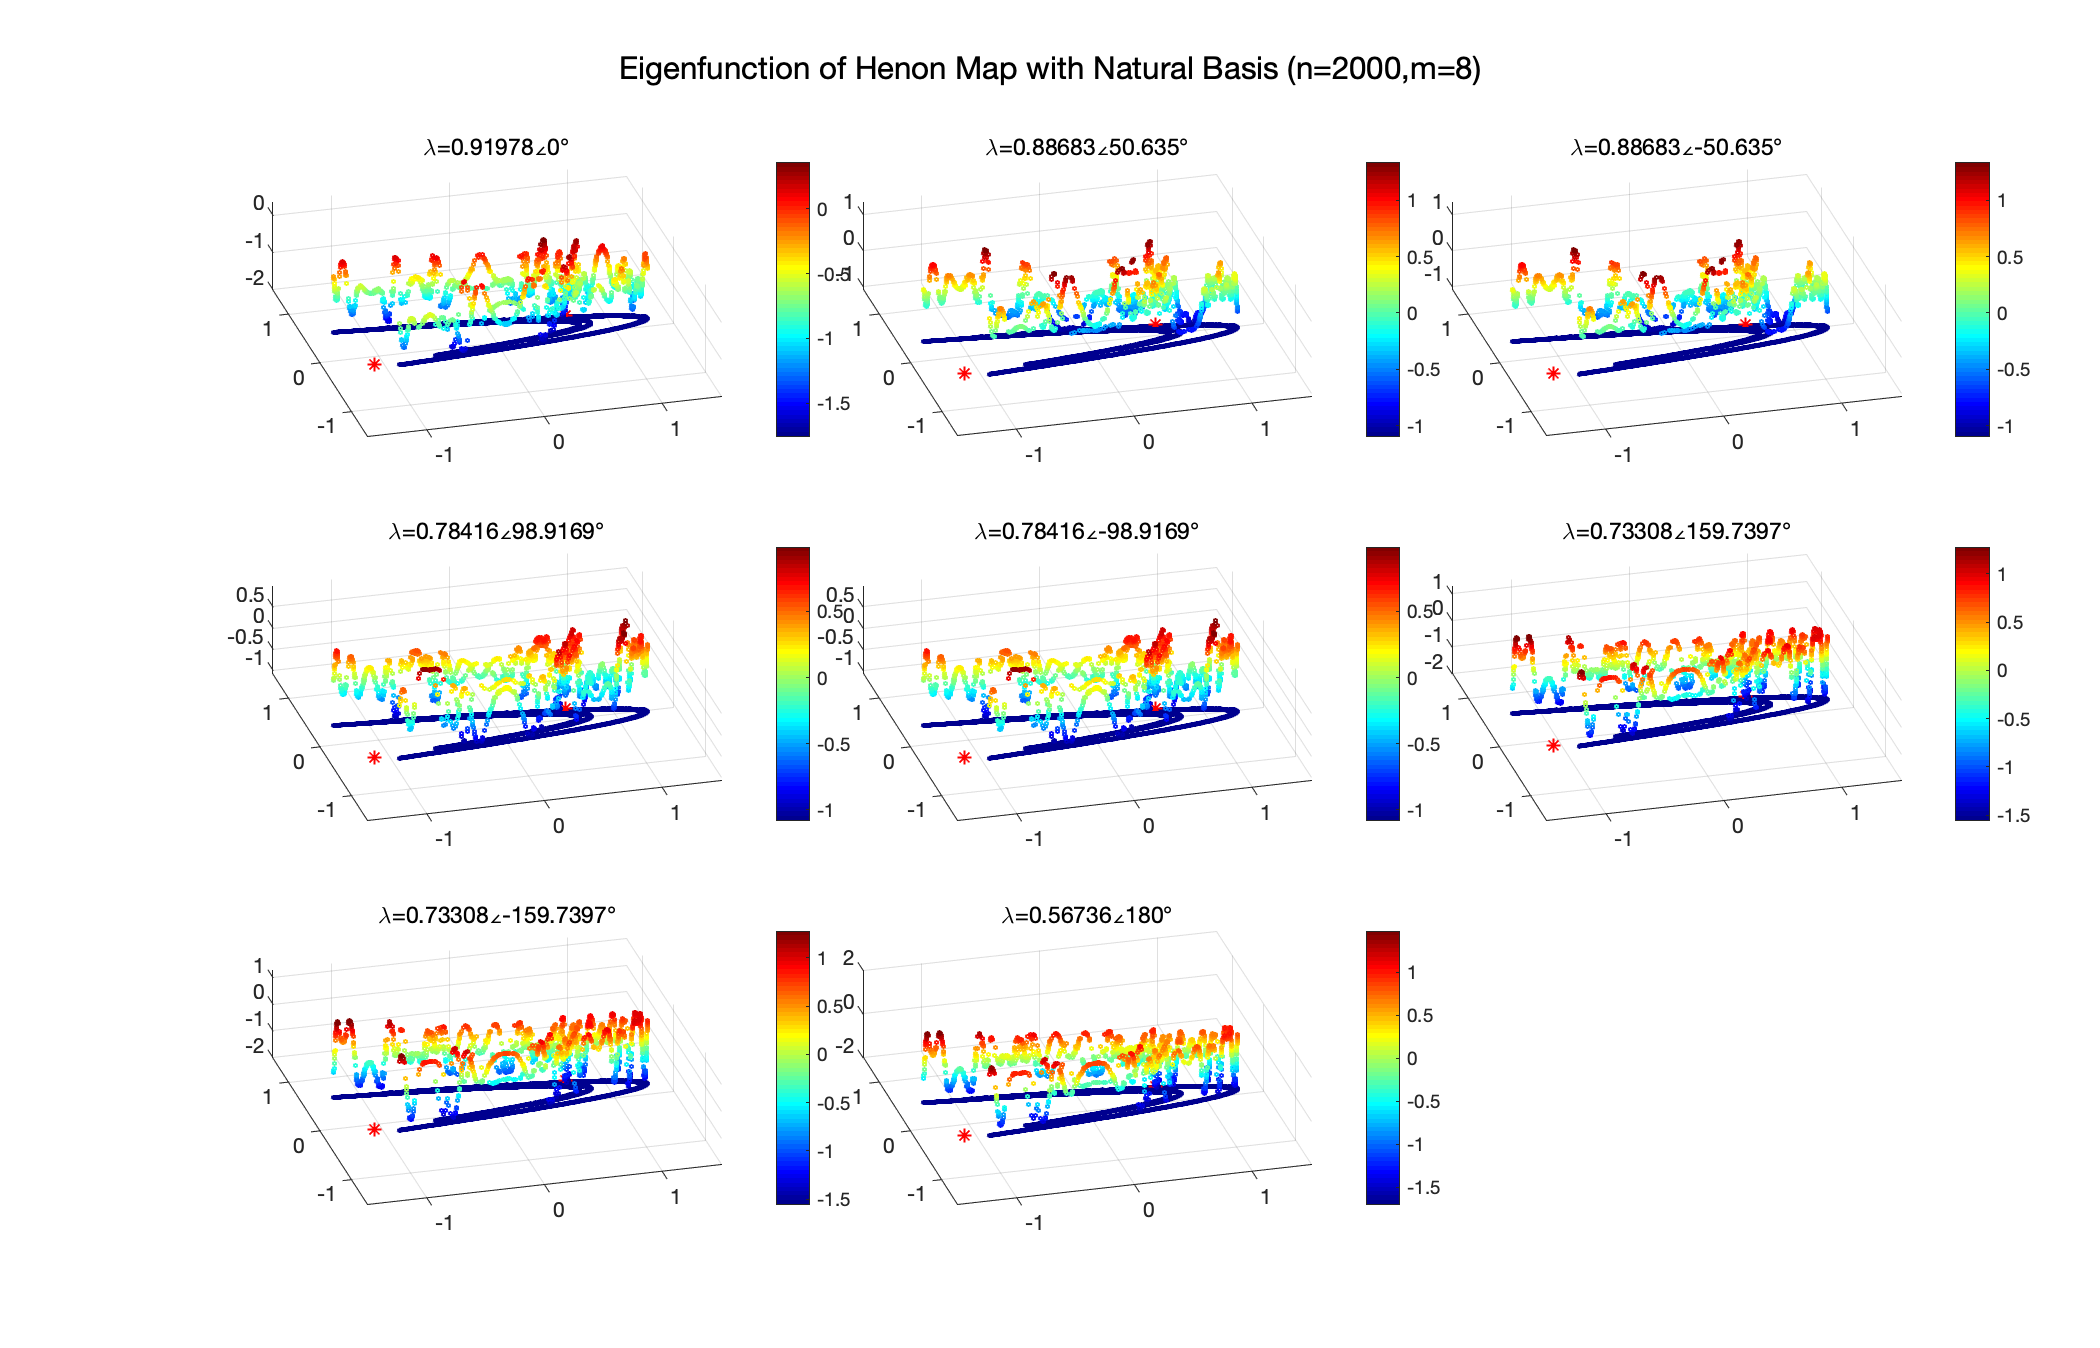
\includegraphics[scale=0.2]{henon/natural/Henon_eigen_natural_n2000m8}}
    \\
    \caption{埃农映射自然基函数不同基函数数量下的本征函数($n=2000$)}
\end{figure}

\begin{figure}
	\centering
	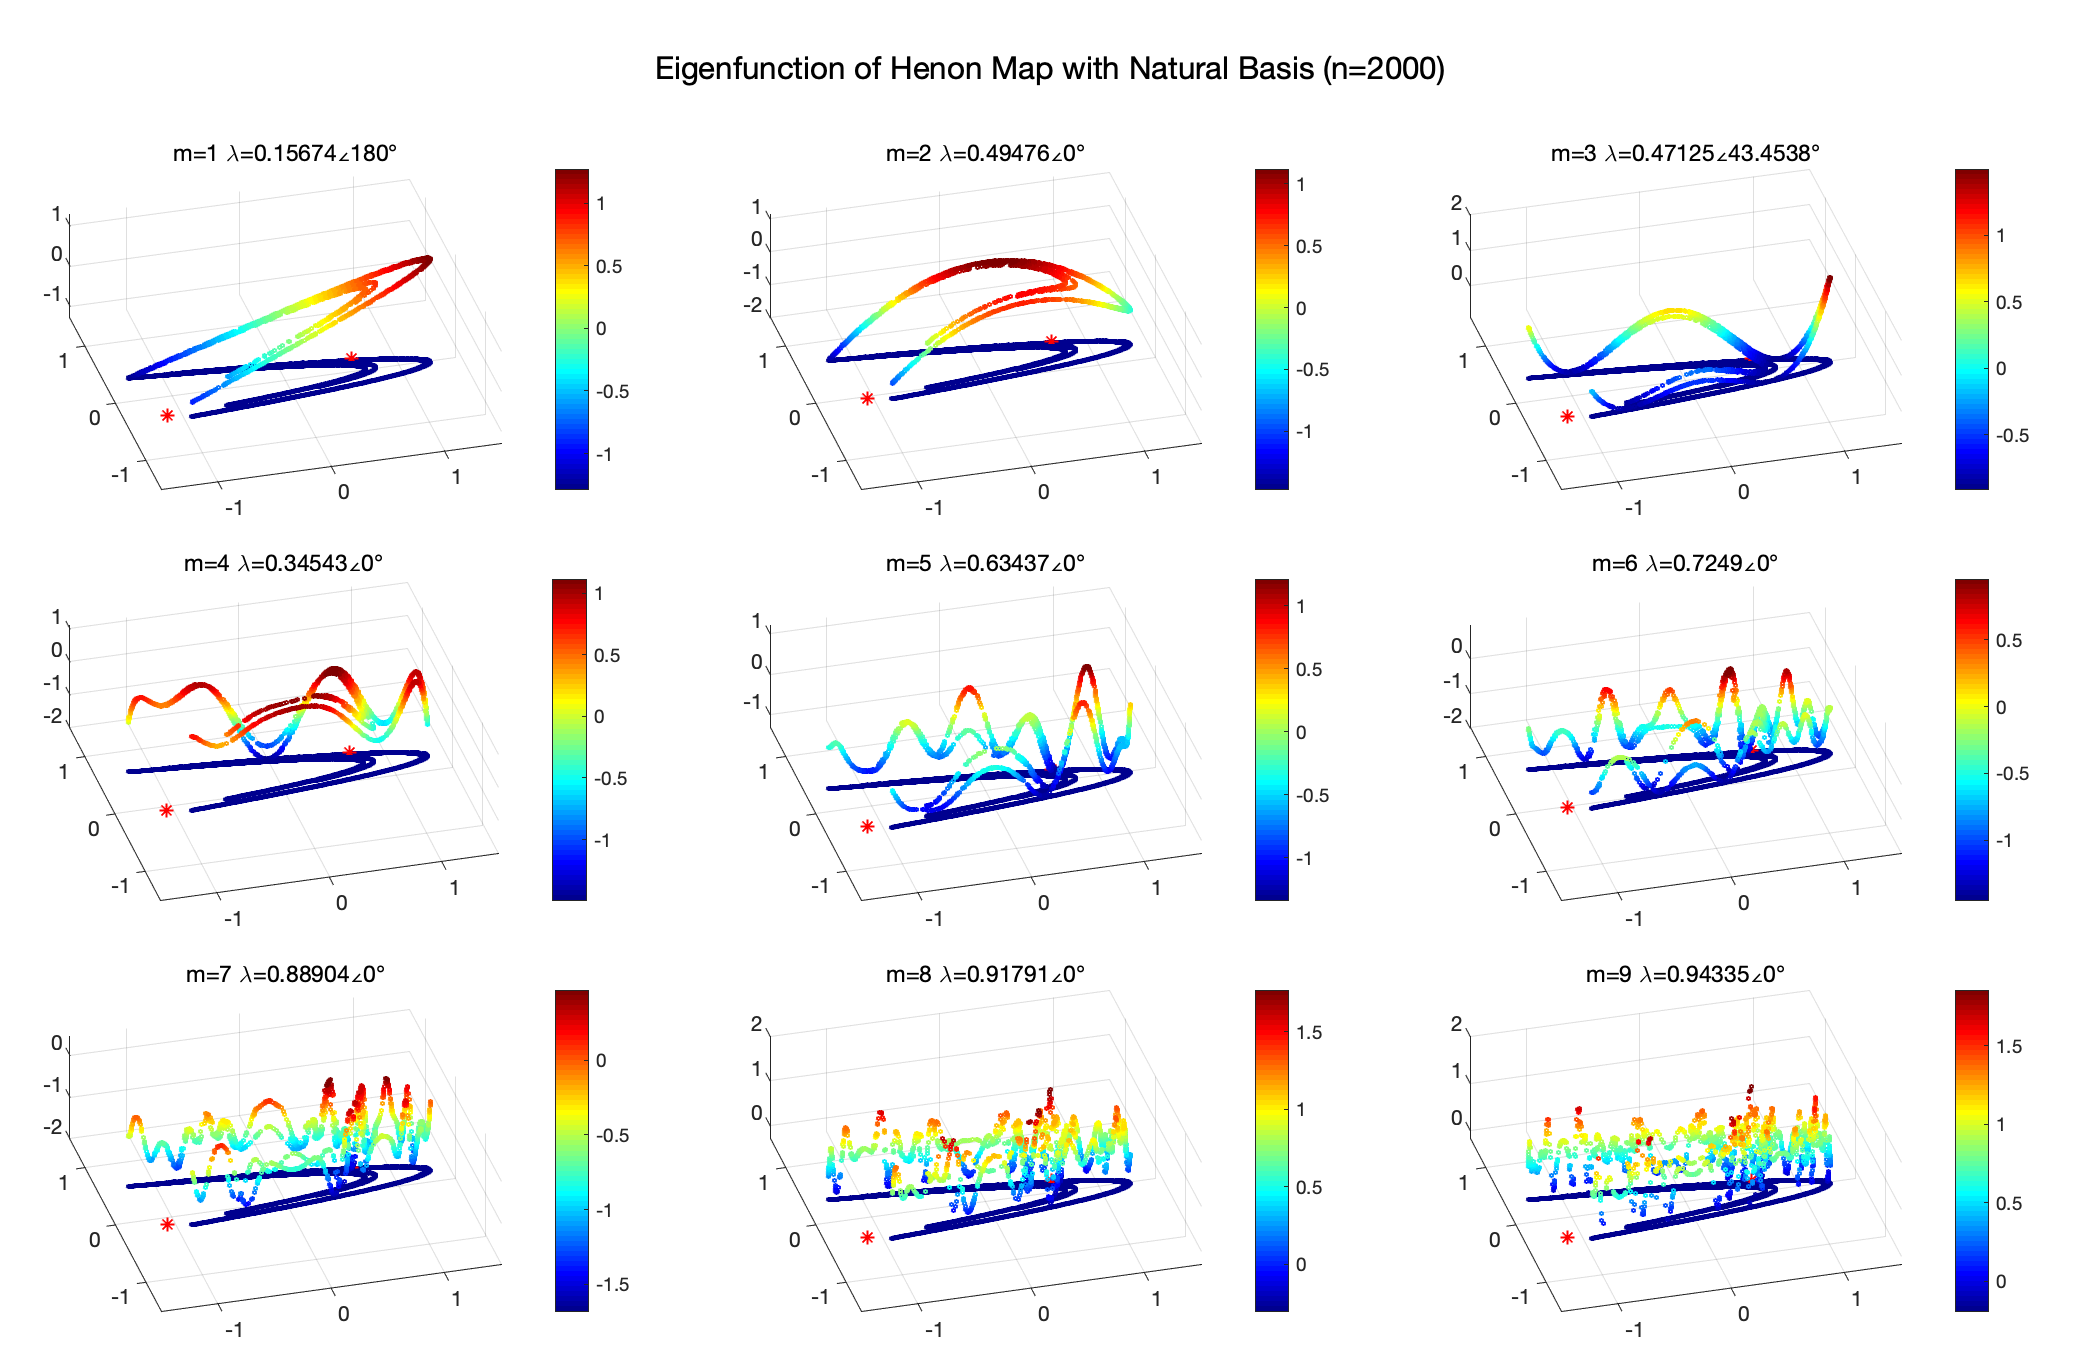
\includegraphics[scale=0.4]{henon/natural/Henon_eigen_natural_n2000}
    \caption{埃农映射自然基函数不同基函数数量下的本征函数($n=2000$)}
\end{figure}

\subsubsection{吸引子上的本征函数}

\begin{figure}
    \centering
    \subfloat[俯视图]{
      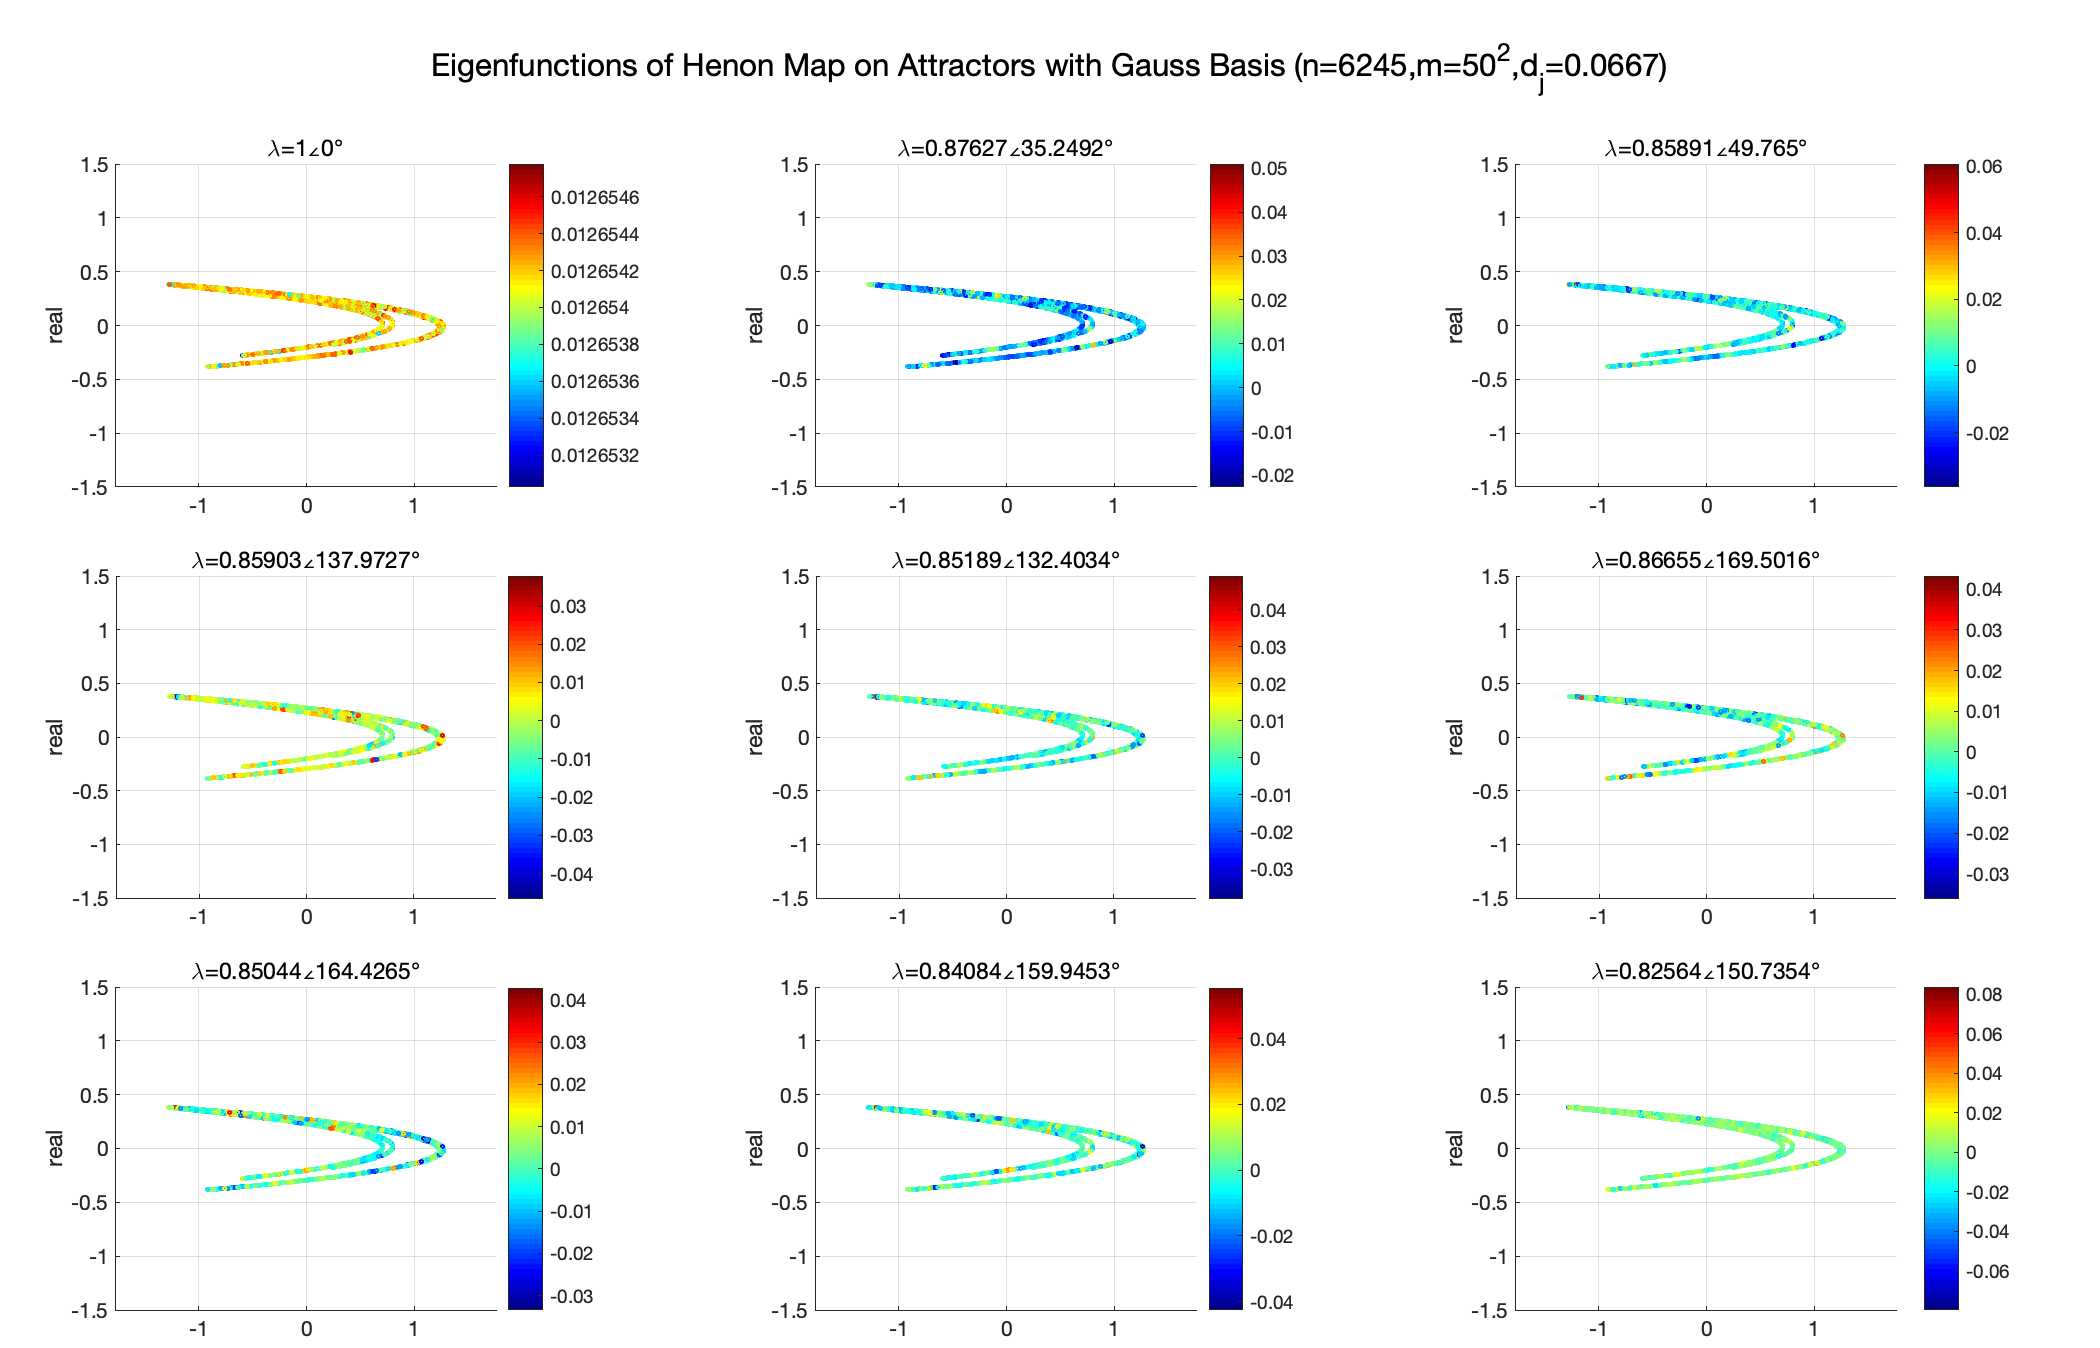
\includegraphics[scale=0.4]{henon/Henon_eigen_Gauss_attr_n6245m50md45}}
    \\
    \subfloat[鸟瞰图]{
      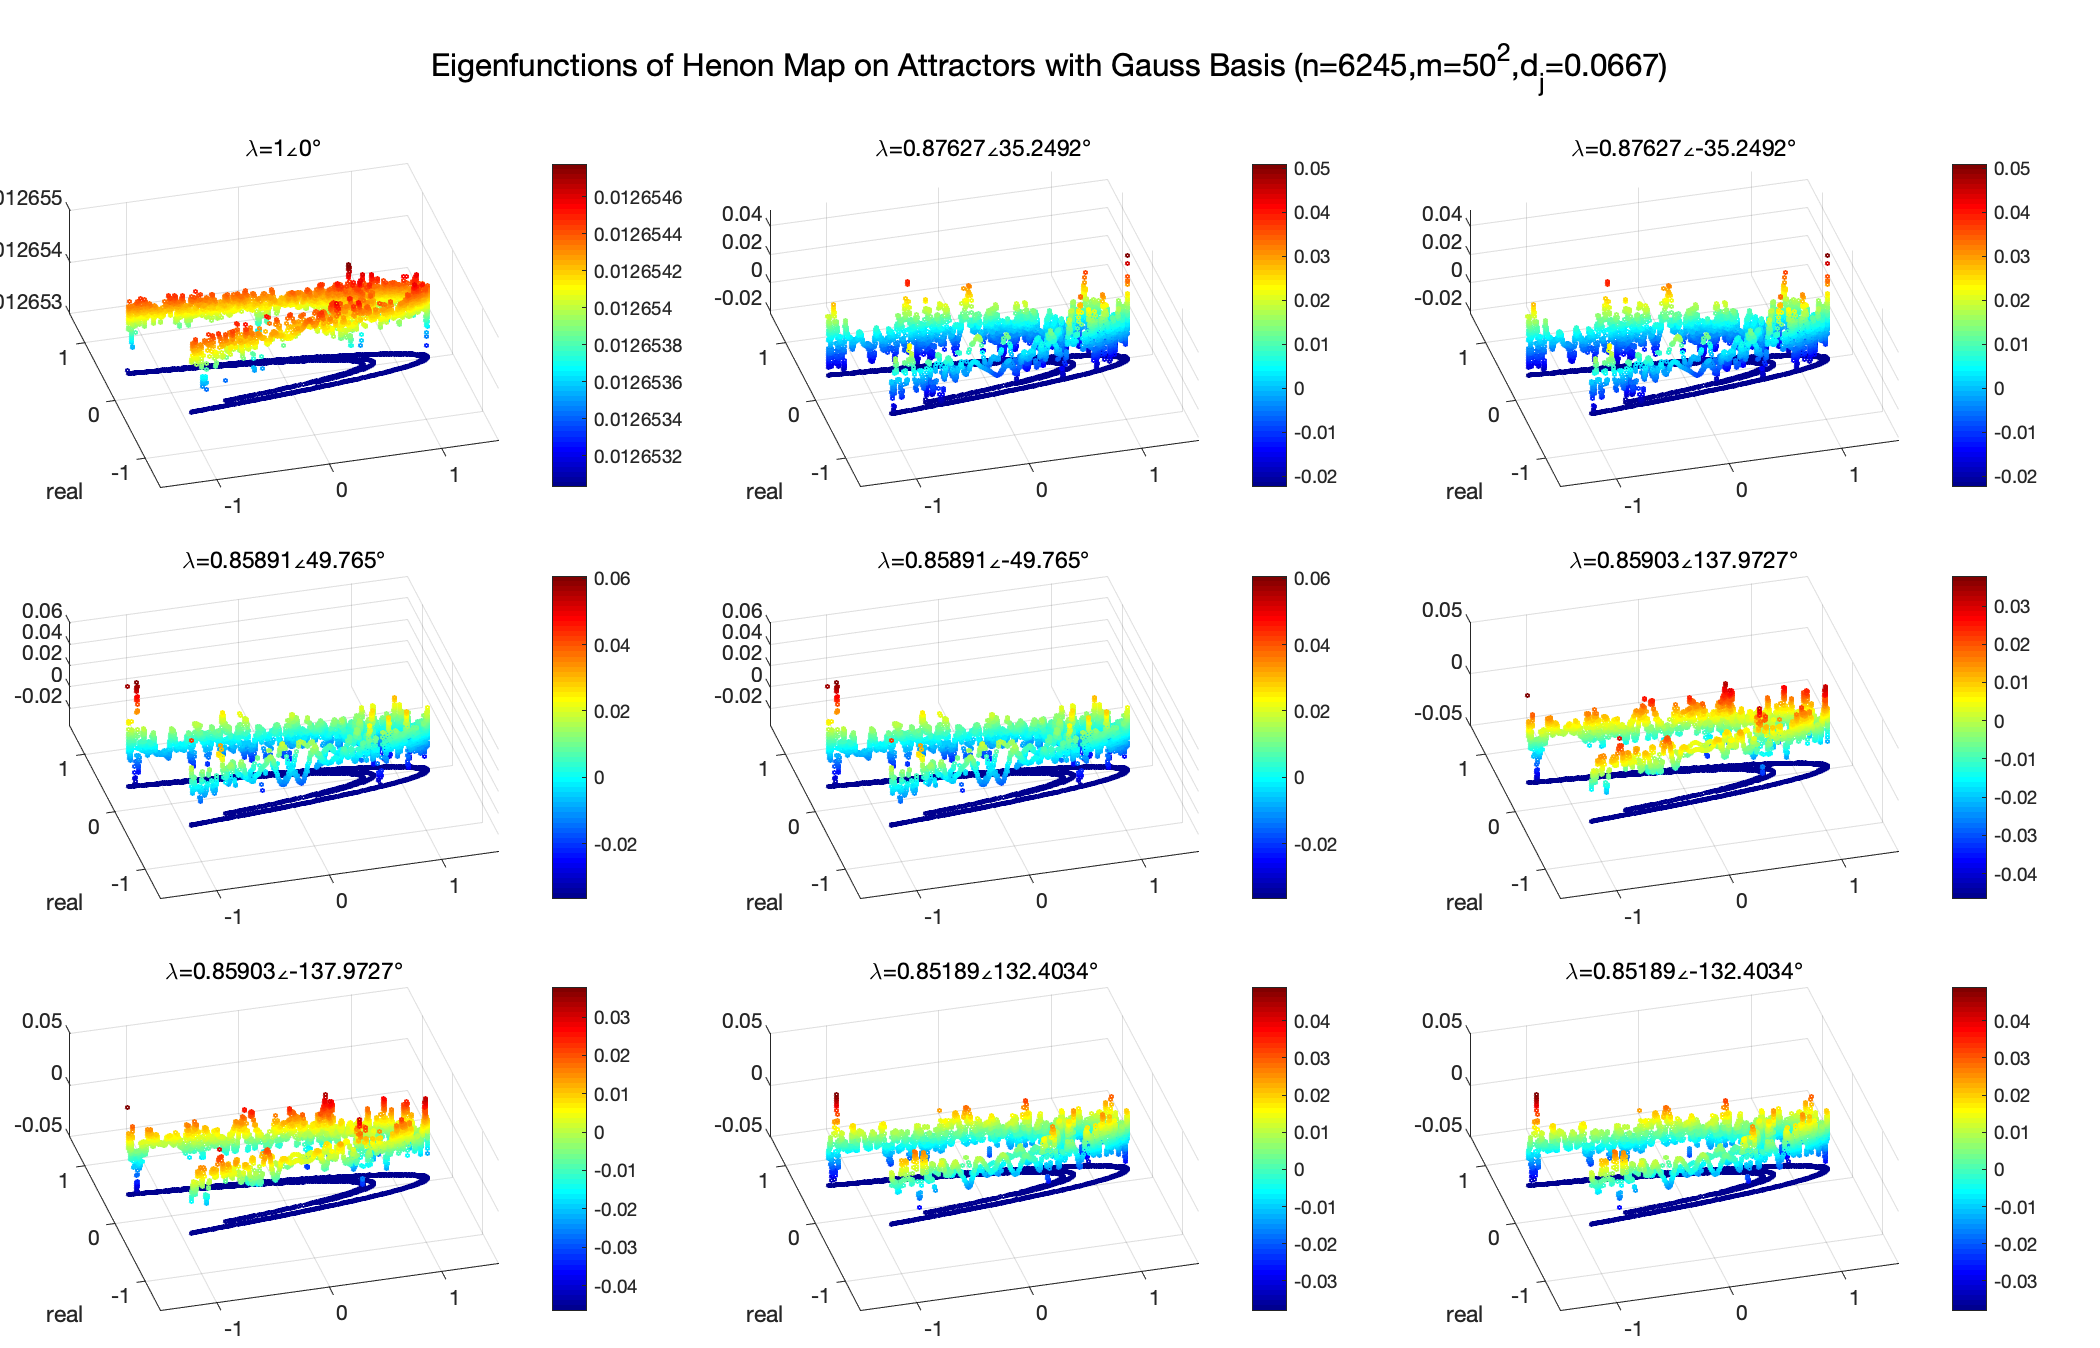
\includegraphics[scale=0.4]{henon/Henon_eigen_Gauss_attr_n6245m50}}
    \\
    \caption{埃农映射高斯基函数下在吸引子上的本征函数($n=6245$,$m=50^2,$,$d_j=\frac{3}{45}$)}
\end{figure}

\begin{figure}
    \centering
    \subfloat[m=2]{
      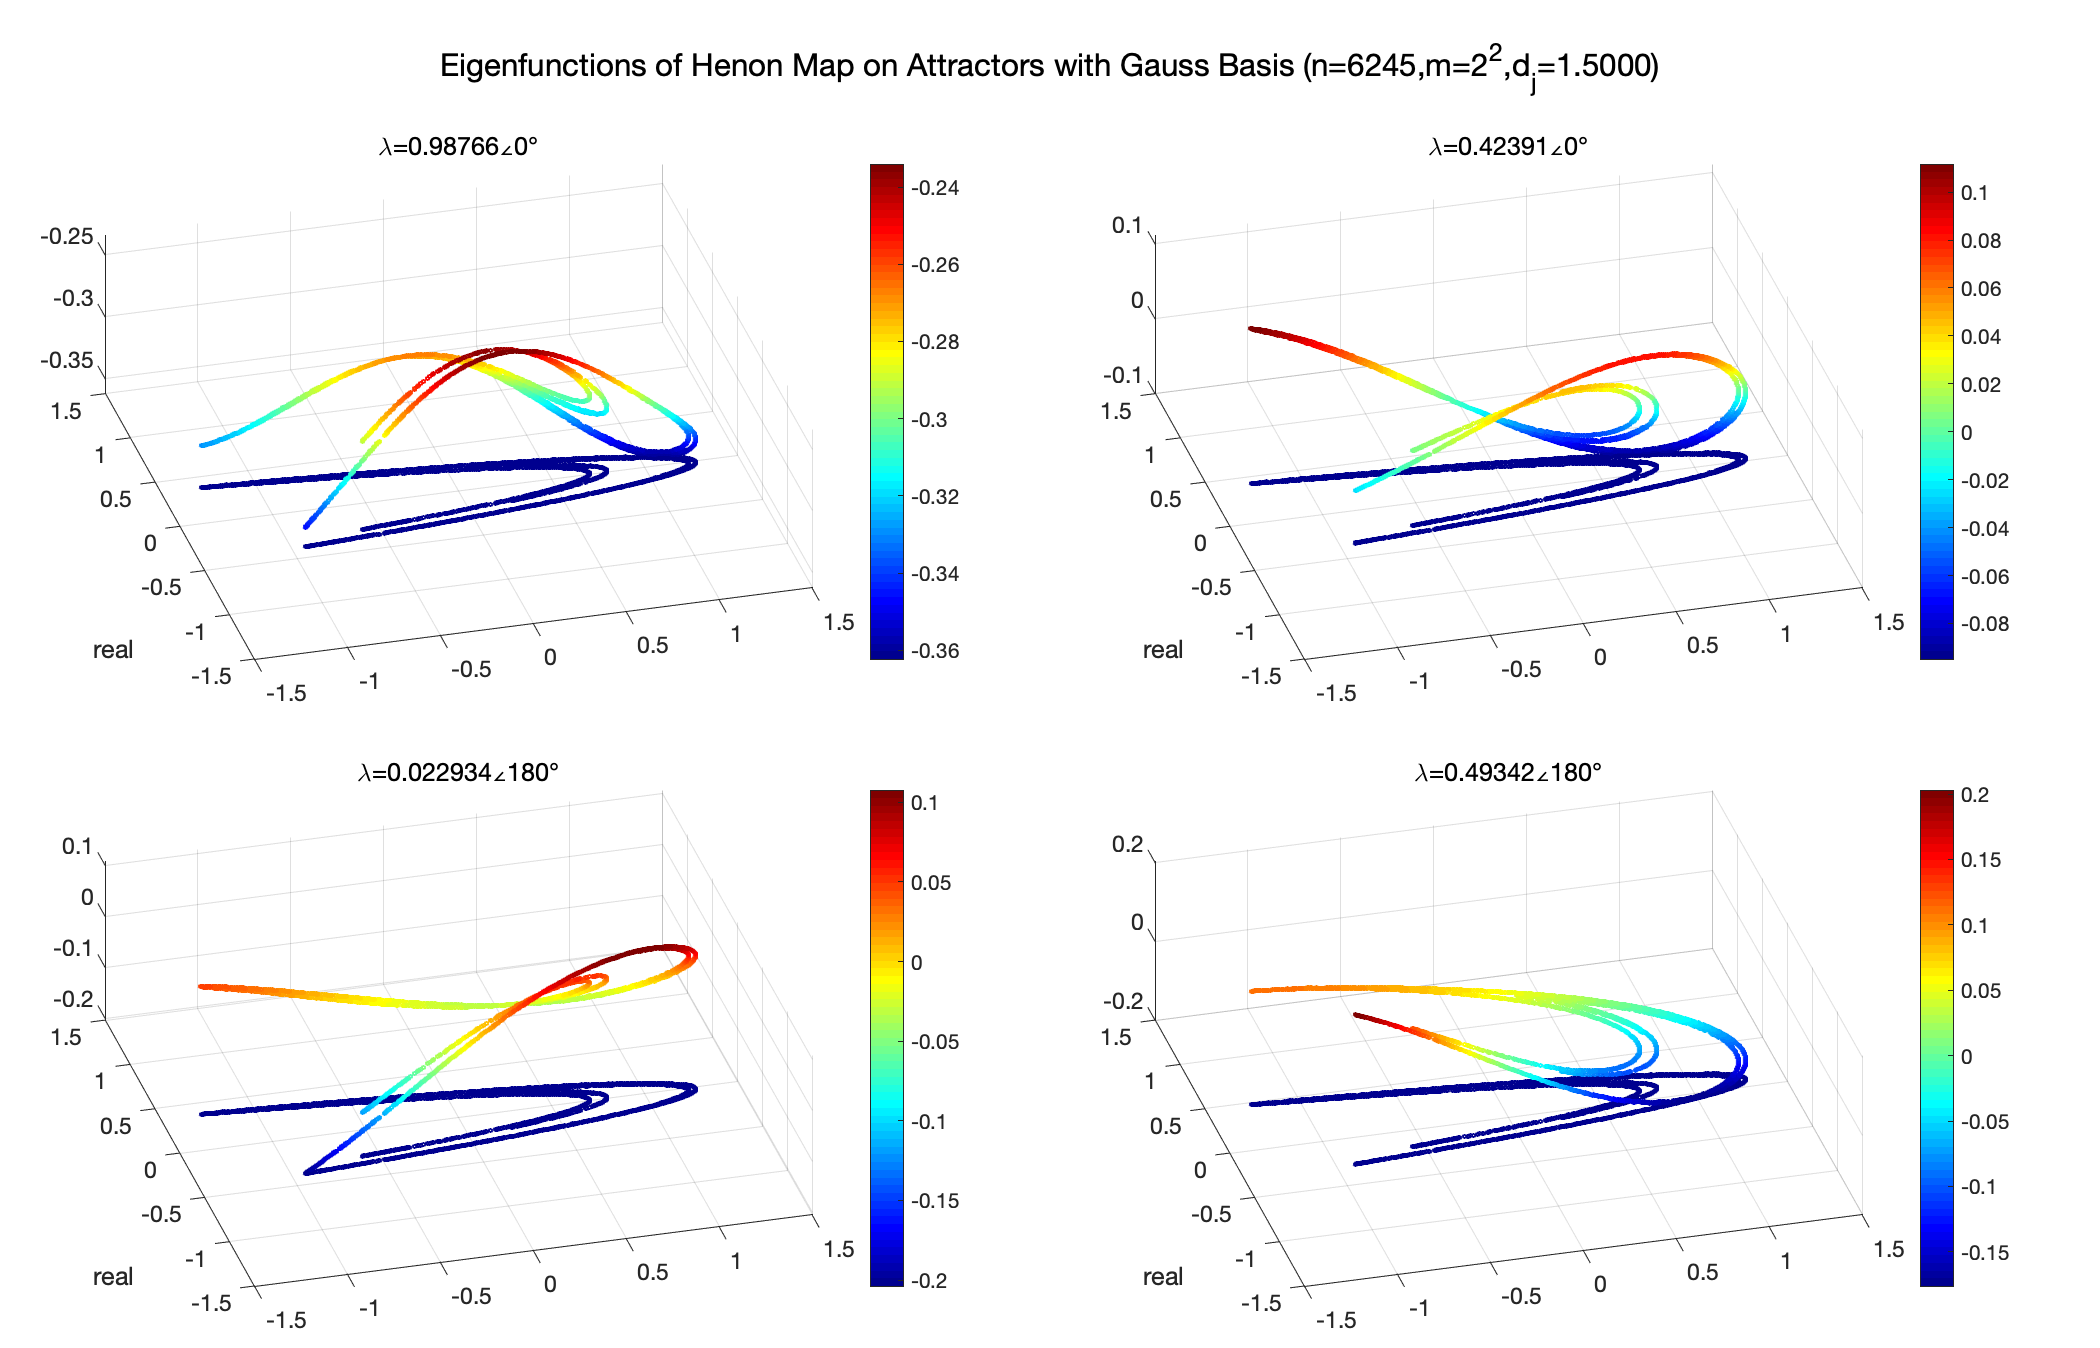
\includegraphics[scale=0.28]{henon/Henon_eigen_Gauss_attr_leftU_n6245m2}}
    \\
    \subfloat[m=3]{
      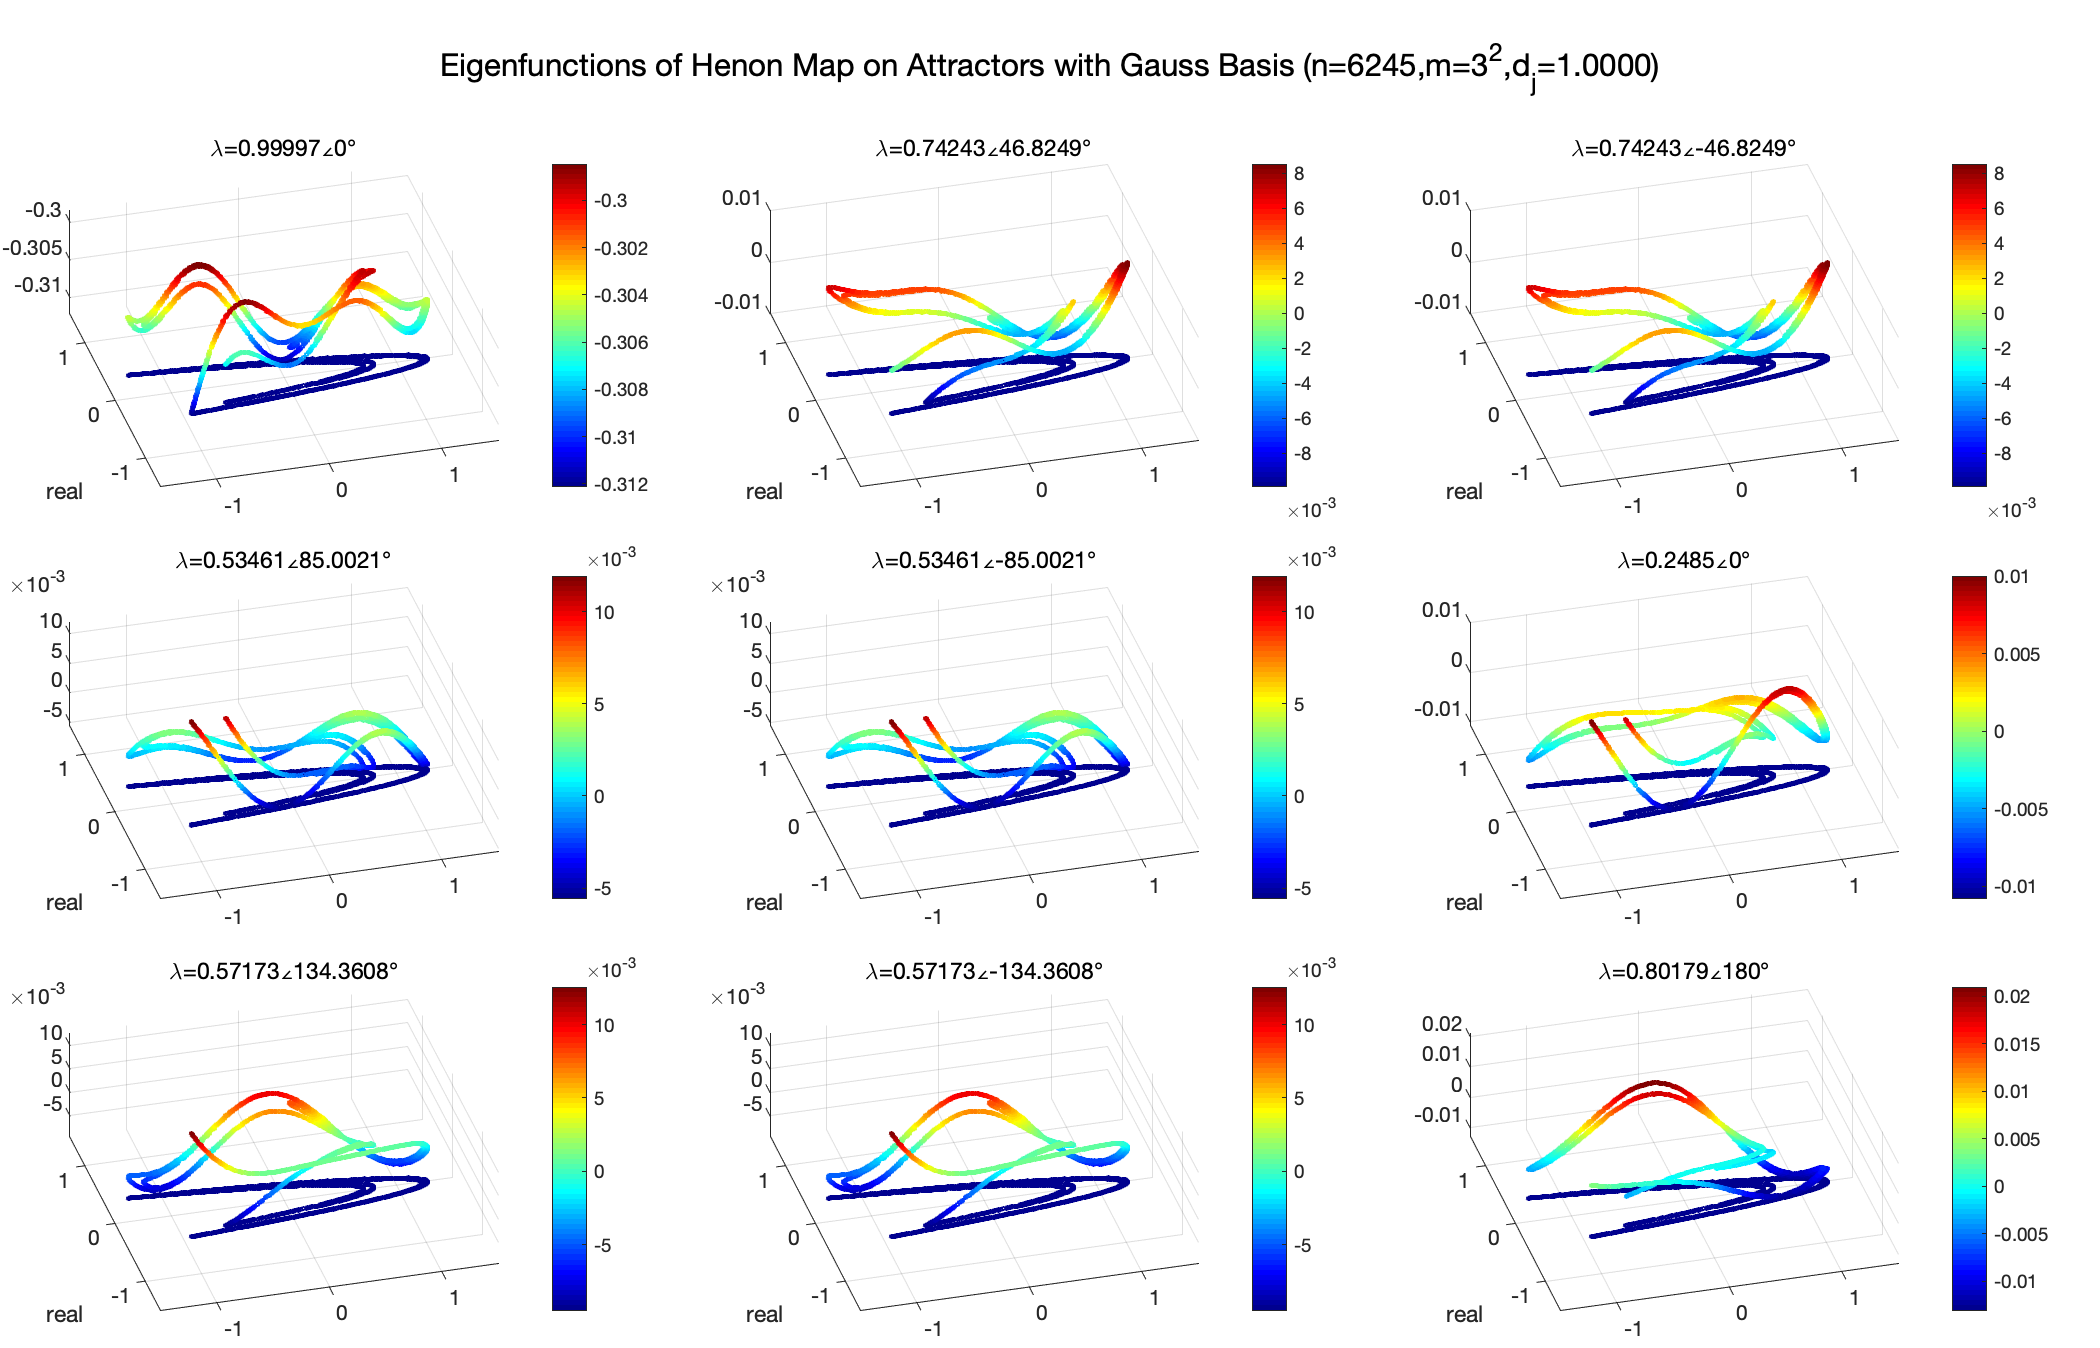
\includegraphics[scale=0.28]{henon/Henon_eigen_Gauss_attr_leftU_n6245m3}}
    \\
    \subfloat[m=4]{
      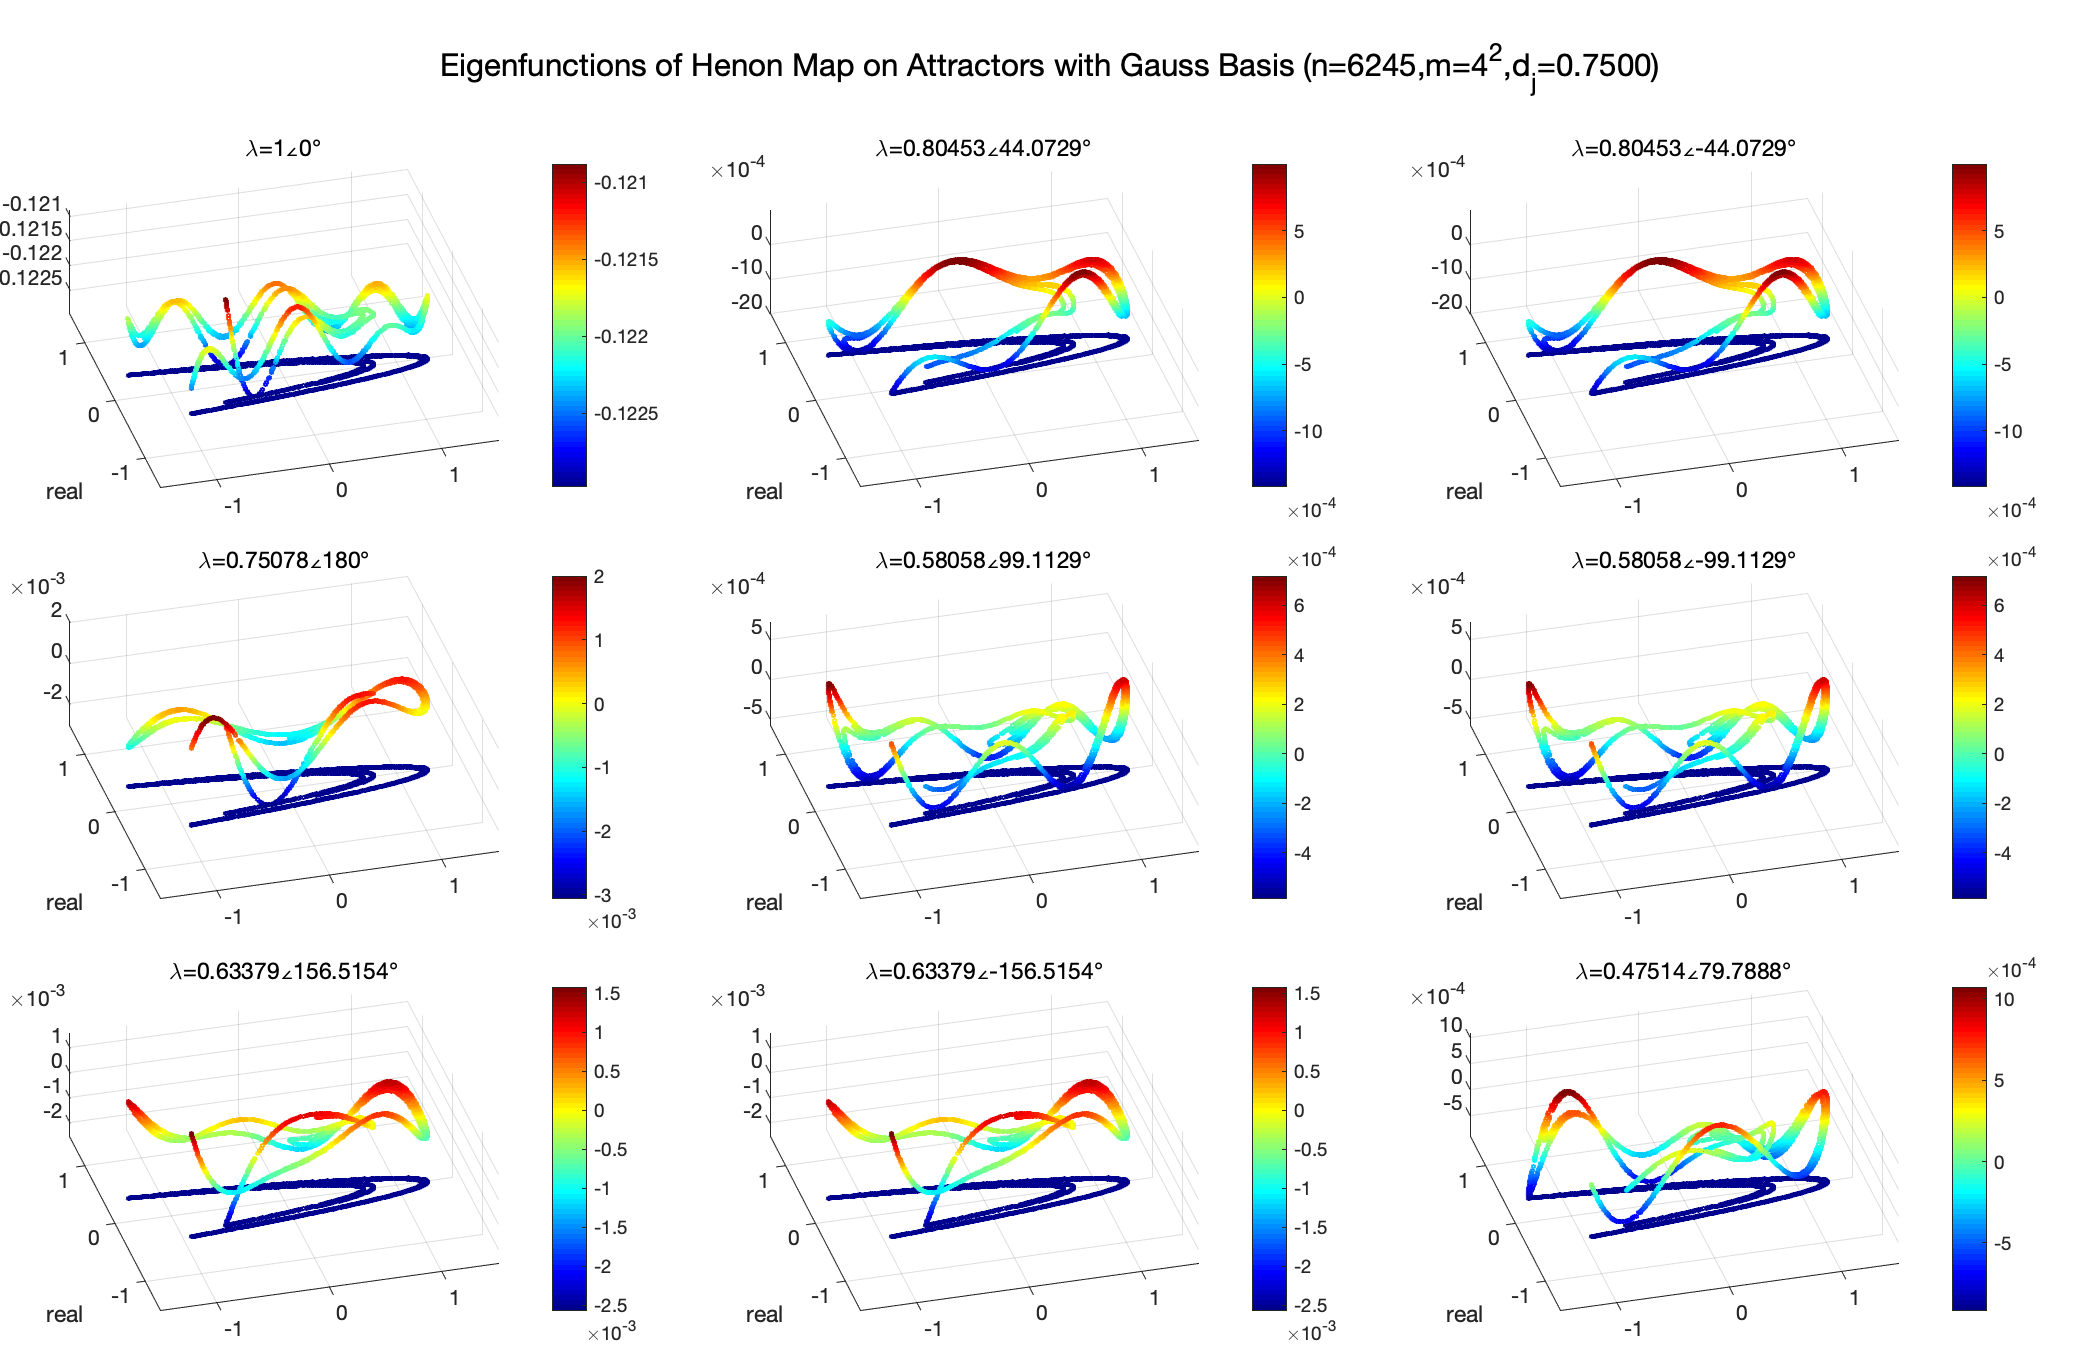
\includegraphics[scale=0.28]{henon/Henon_eigen_Gauss_attr_leftU_n6245m4}}
    \\
    \caption{埃农映射高斯基函数下在吸引子上的本征函数($n=6245$)}
\end{figure}


\subsection{Koopman算符对埃农映射的相空间划分}
\subsubsection{埃农映射在吸引子上的划分}
\begin{table}[]
    \centering
    \begin{tabular}{|c|c|c|}
    \hline
        & 横坐标x & 纵坐标y  \\ \hline
    1   & 0.7021 & -0.0044 \\ \hline
    2   & 0.7986 & 0.0019  \\ \hline
    3   & 1.2307 & -0.0249 \\ \hline
    4   & 1.2717 & -0.0205 \\ \hline
    \end{tabular}
    \caption{埃农映射的边界点}
\end{table}

\begin{figure}
	\centering
	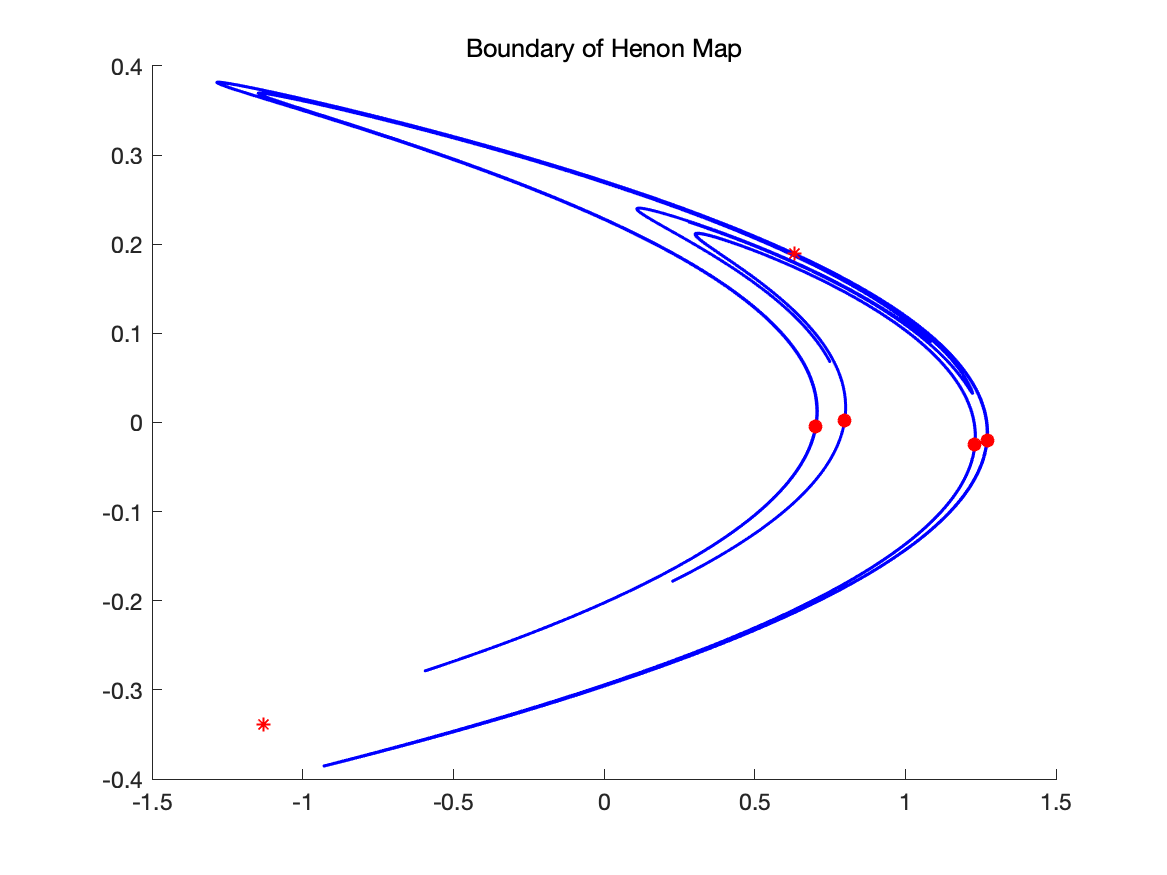
\includegraphics[scale=0.6]{henon/attractors/Henon_boundary}
    \caption{埃农映射的边界点}
\end{figure}

\begin{figure}
    \centering
    \subfloat[正向迭代]{
      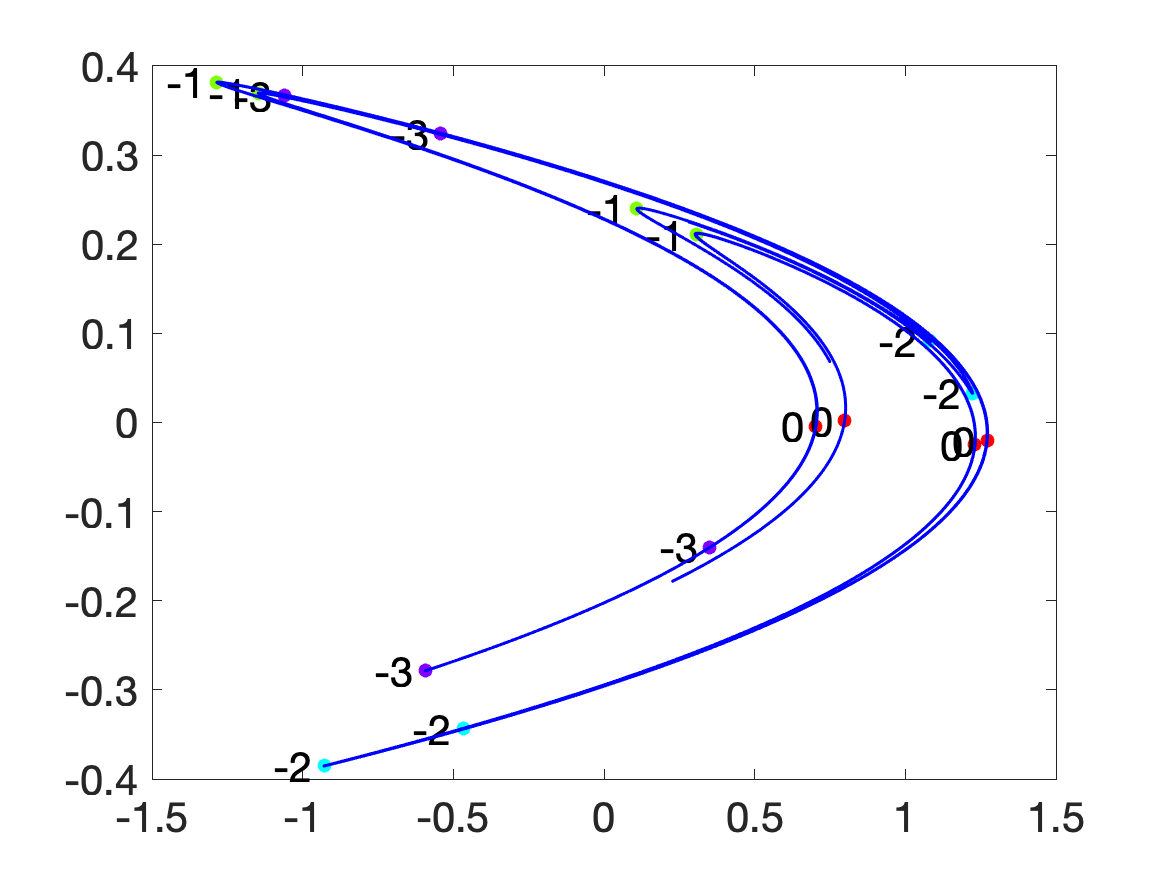
\includegraphics[scale=0.4]{henon/attractors/Henon_boundary_forward}}
    \subfloat[反向迭代]{
      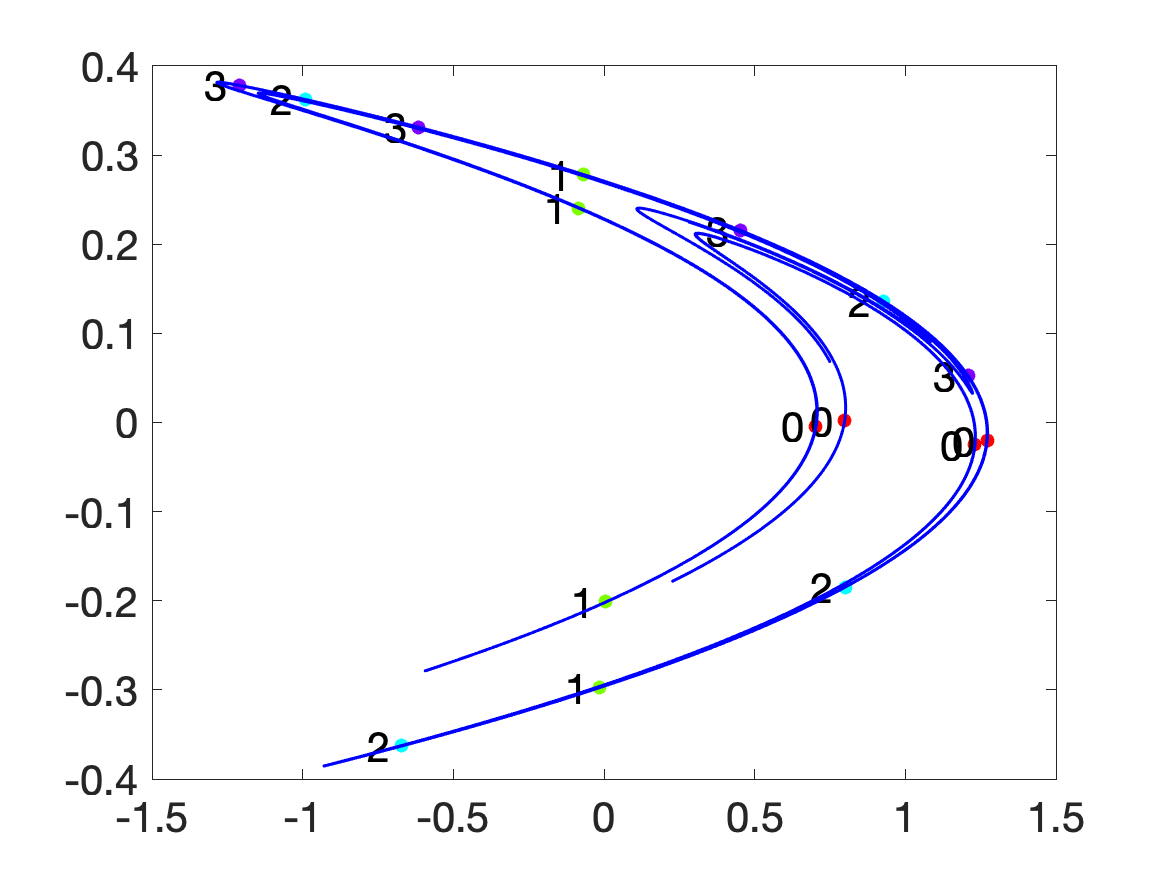
\includegraphics[scale=0.4]{henon/attractors/Henon_boundary_reverse}}
    \caption{埃农映射的边界点及其像点、原像点}
\end{figure}

\begin{figure}
    \centering
    \subfloat[m=1]{
      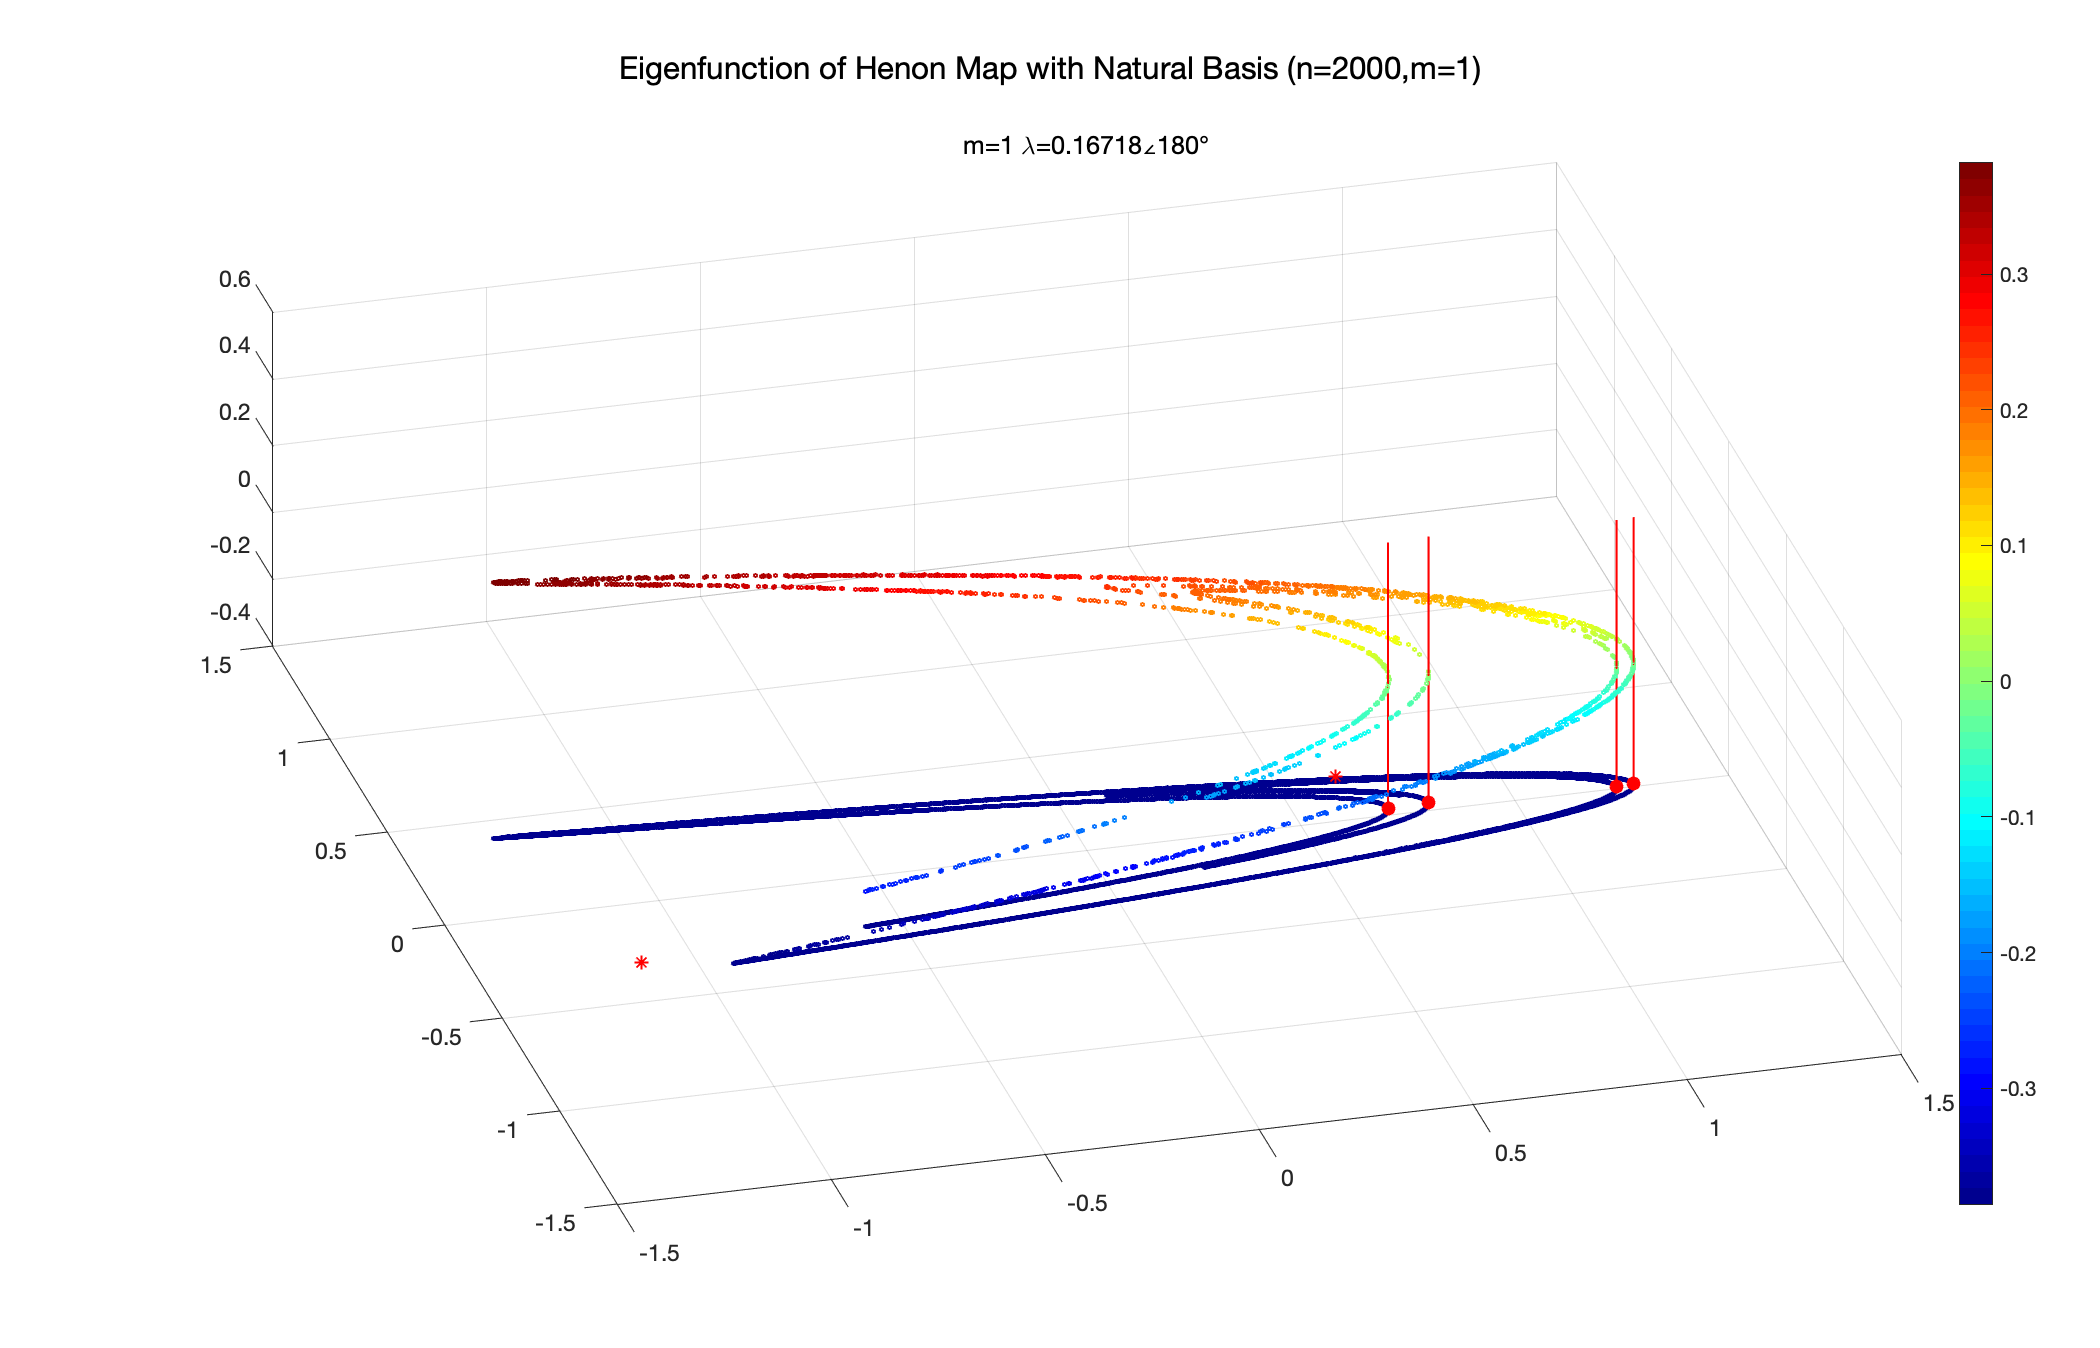
\includegraphics[scale=0.2]{henon/attractors/Henon_eigen_natural_attr_n2000m1}}
    \subfloat[m=2]{
      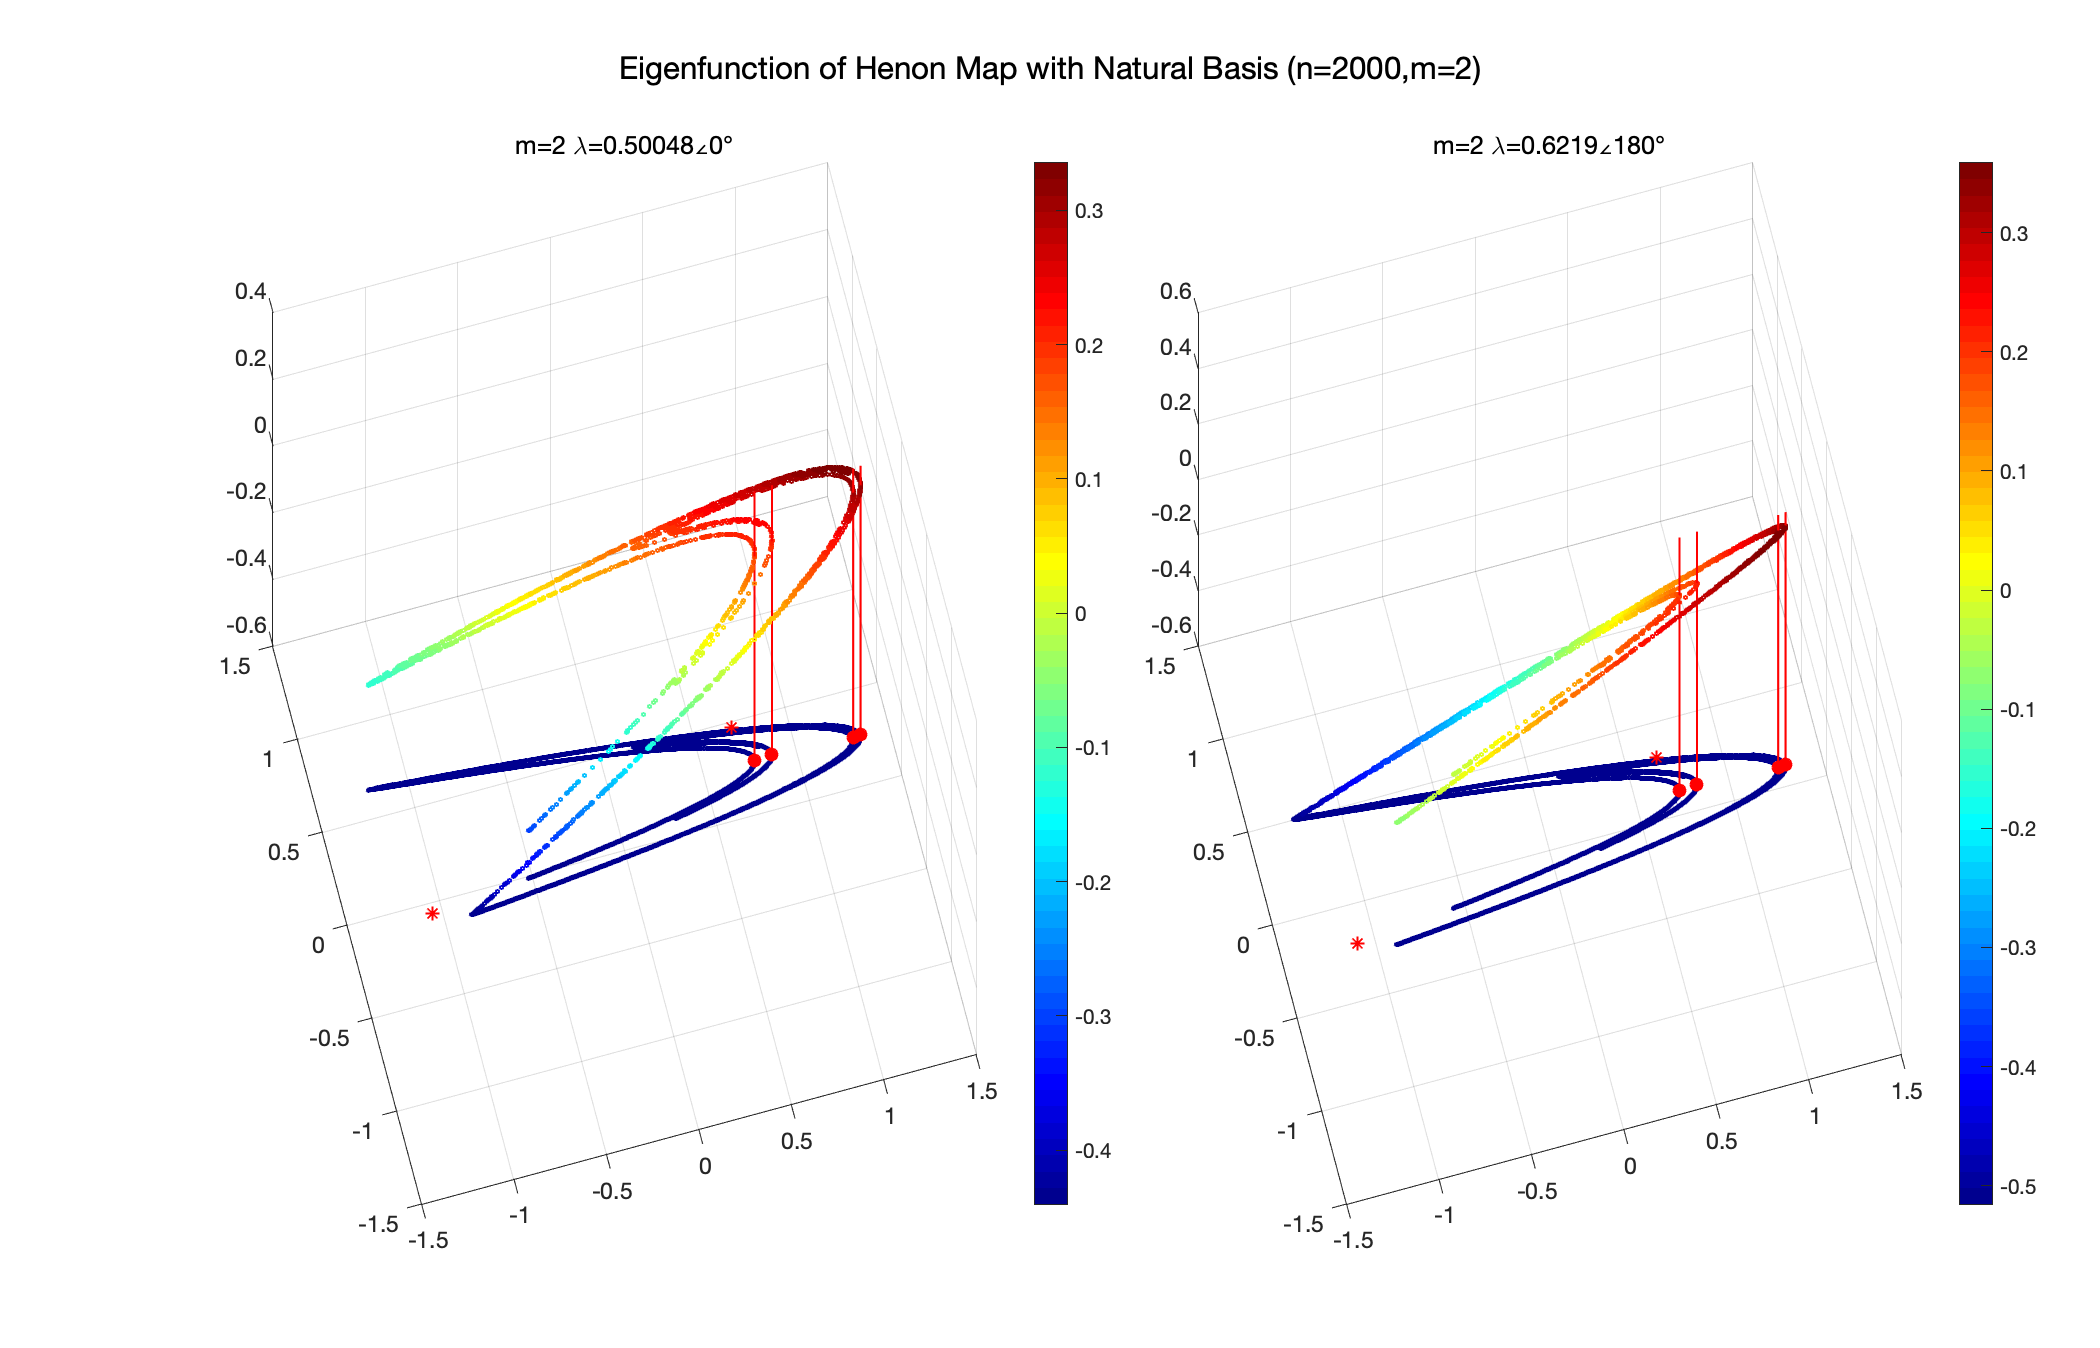
\includegraphics[scale=0.2]{henon/attractors/Henon_eigen_natural_attr_n2000m2}}
    \\
    \subfloat[m=3]{
      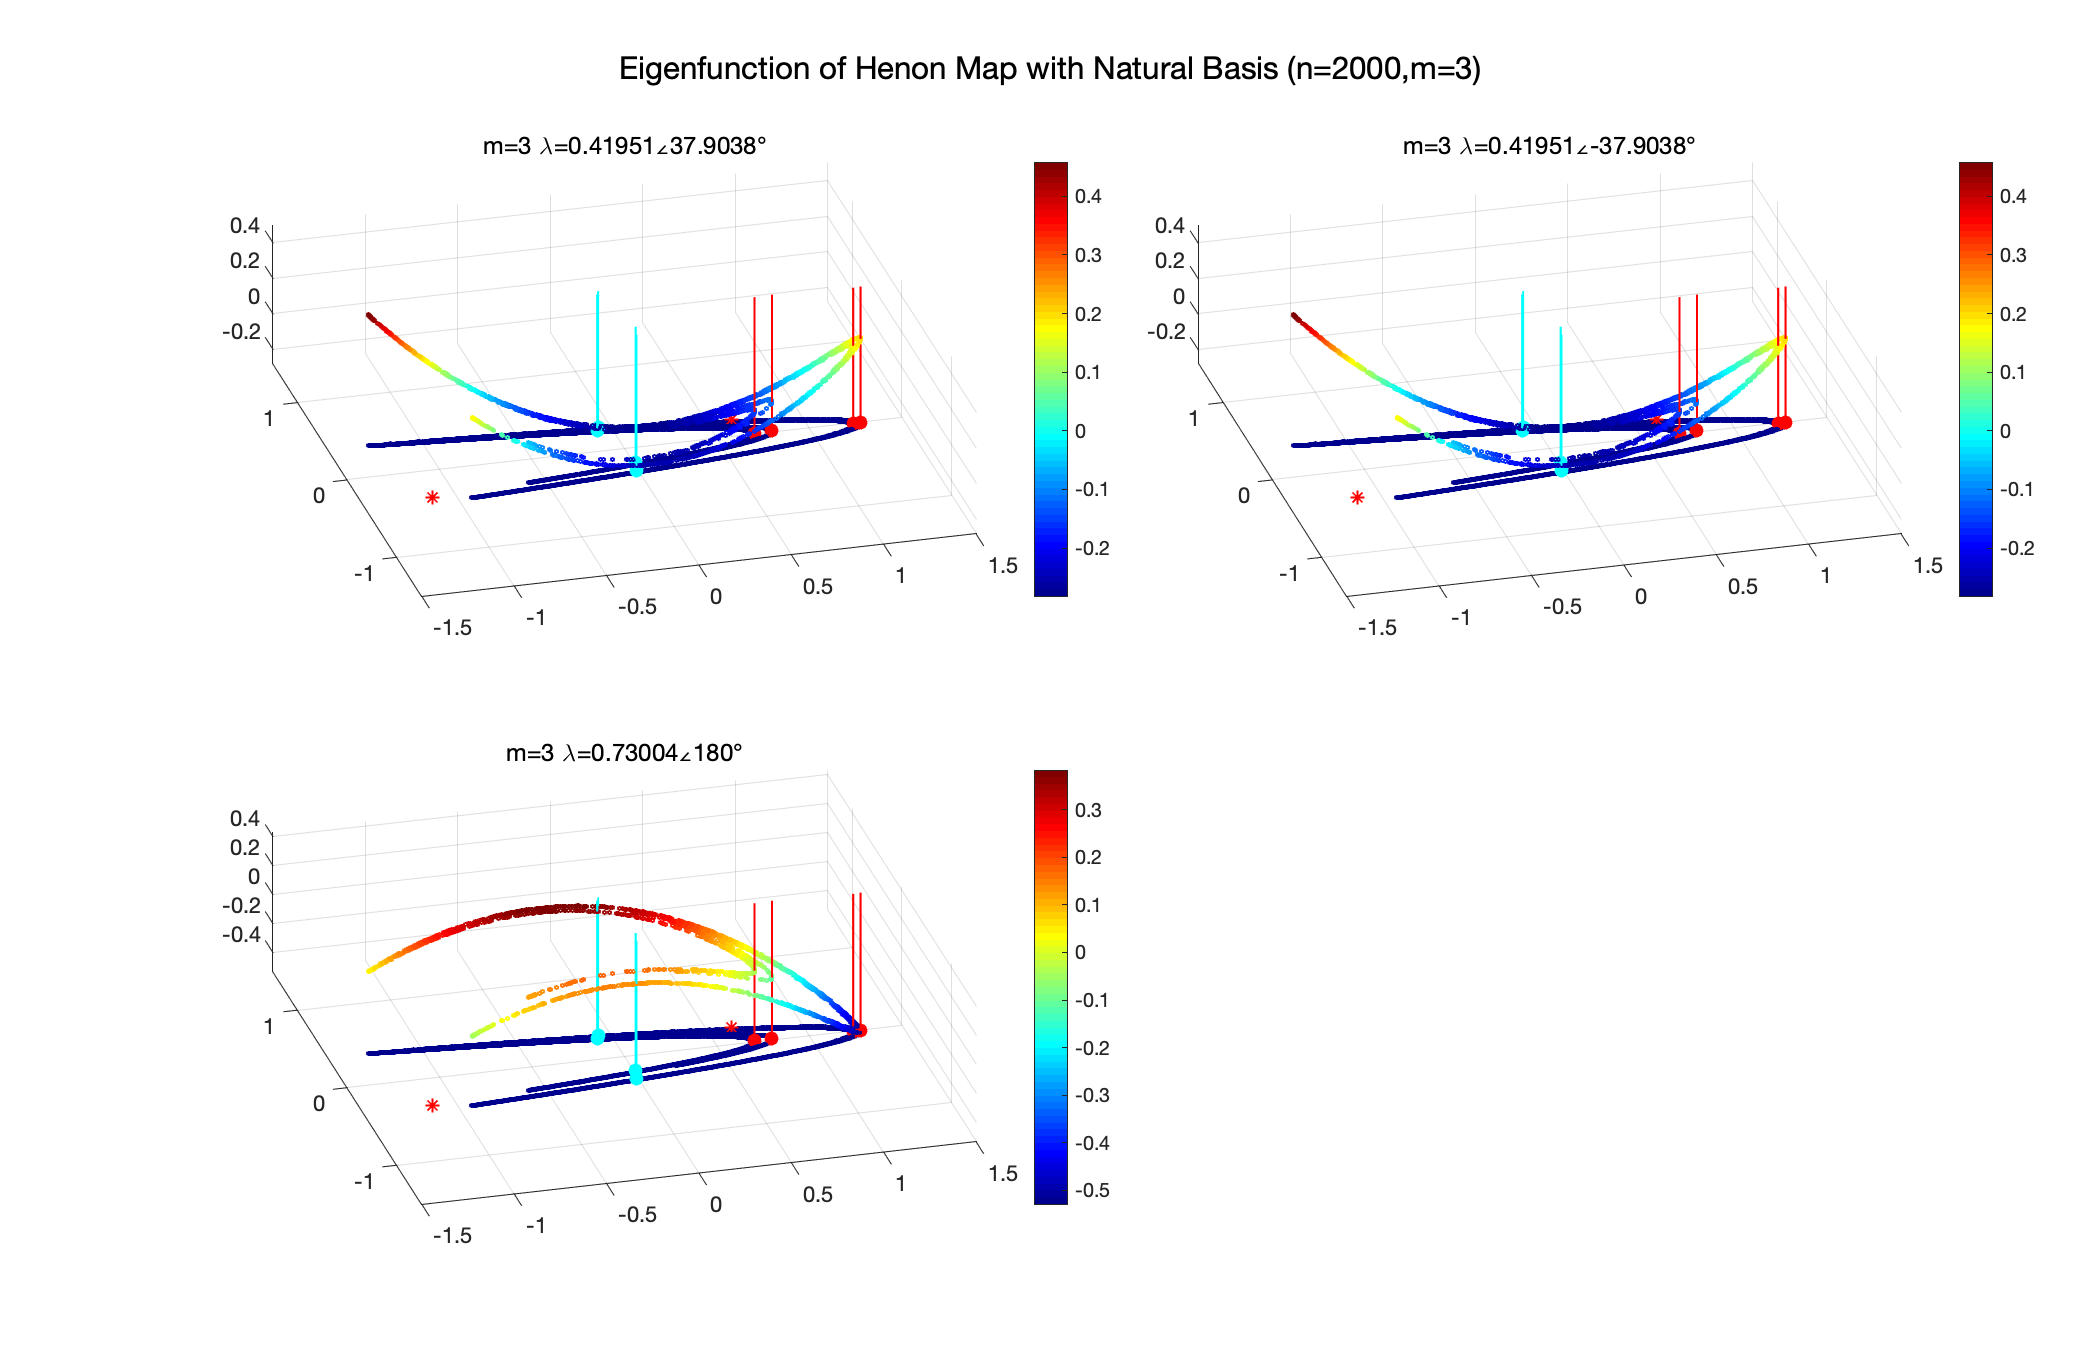
\includegraphics[scale=0.2]{henon/attractors/Henon_eigen_natural_attr_n2000m3}}
    \subfloat[m=4]{
      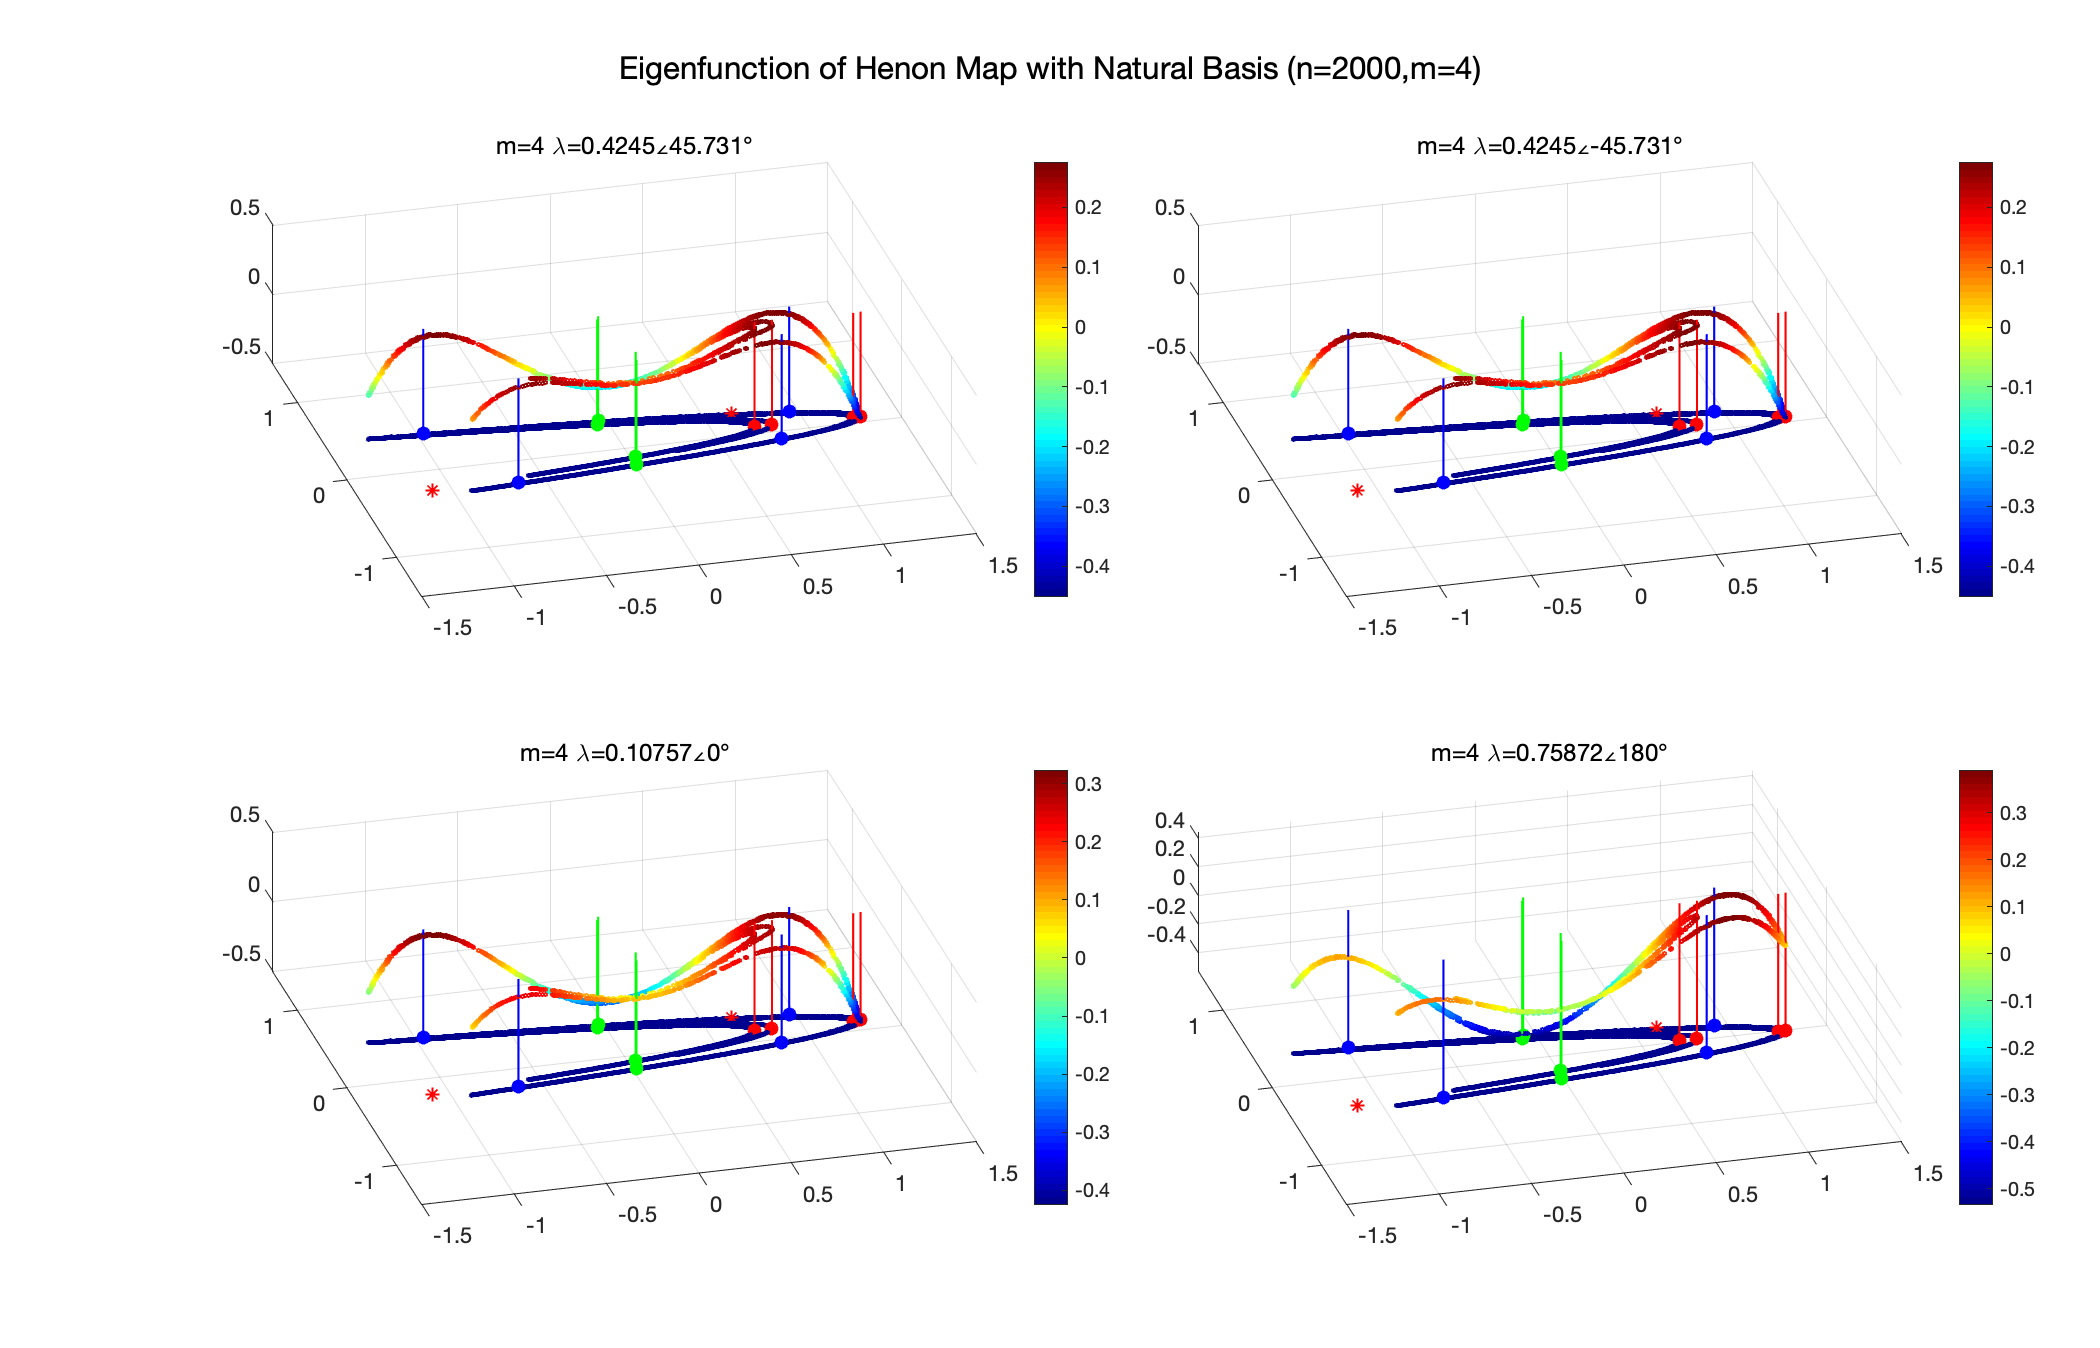
\includegraphics[scale=0.2]{henon/attractors/Henon_eigen_natural_attr_n2000m4}}
    \\
    \subfloat[m=5]{
      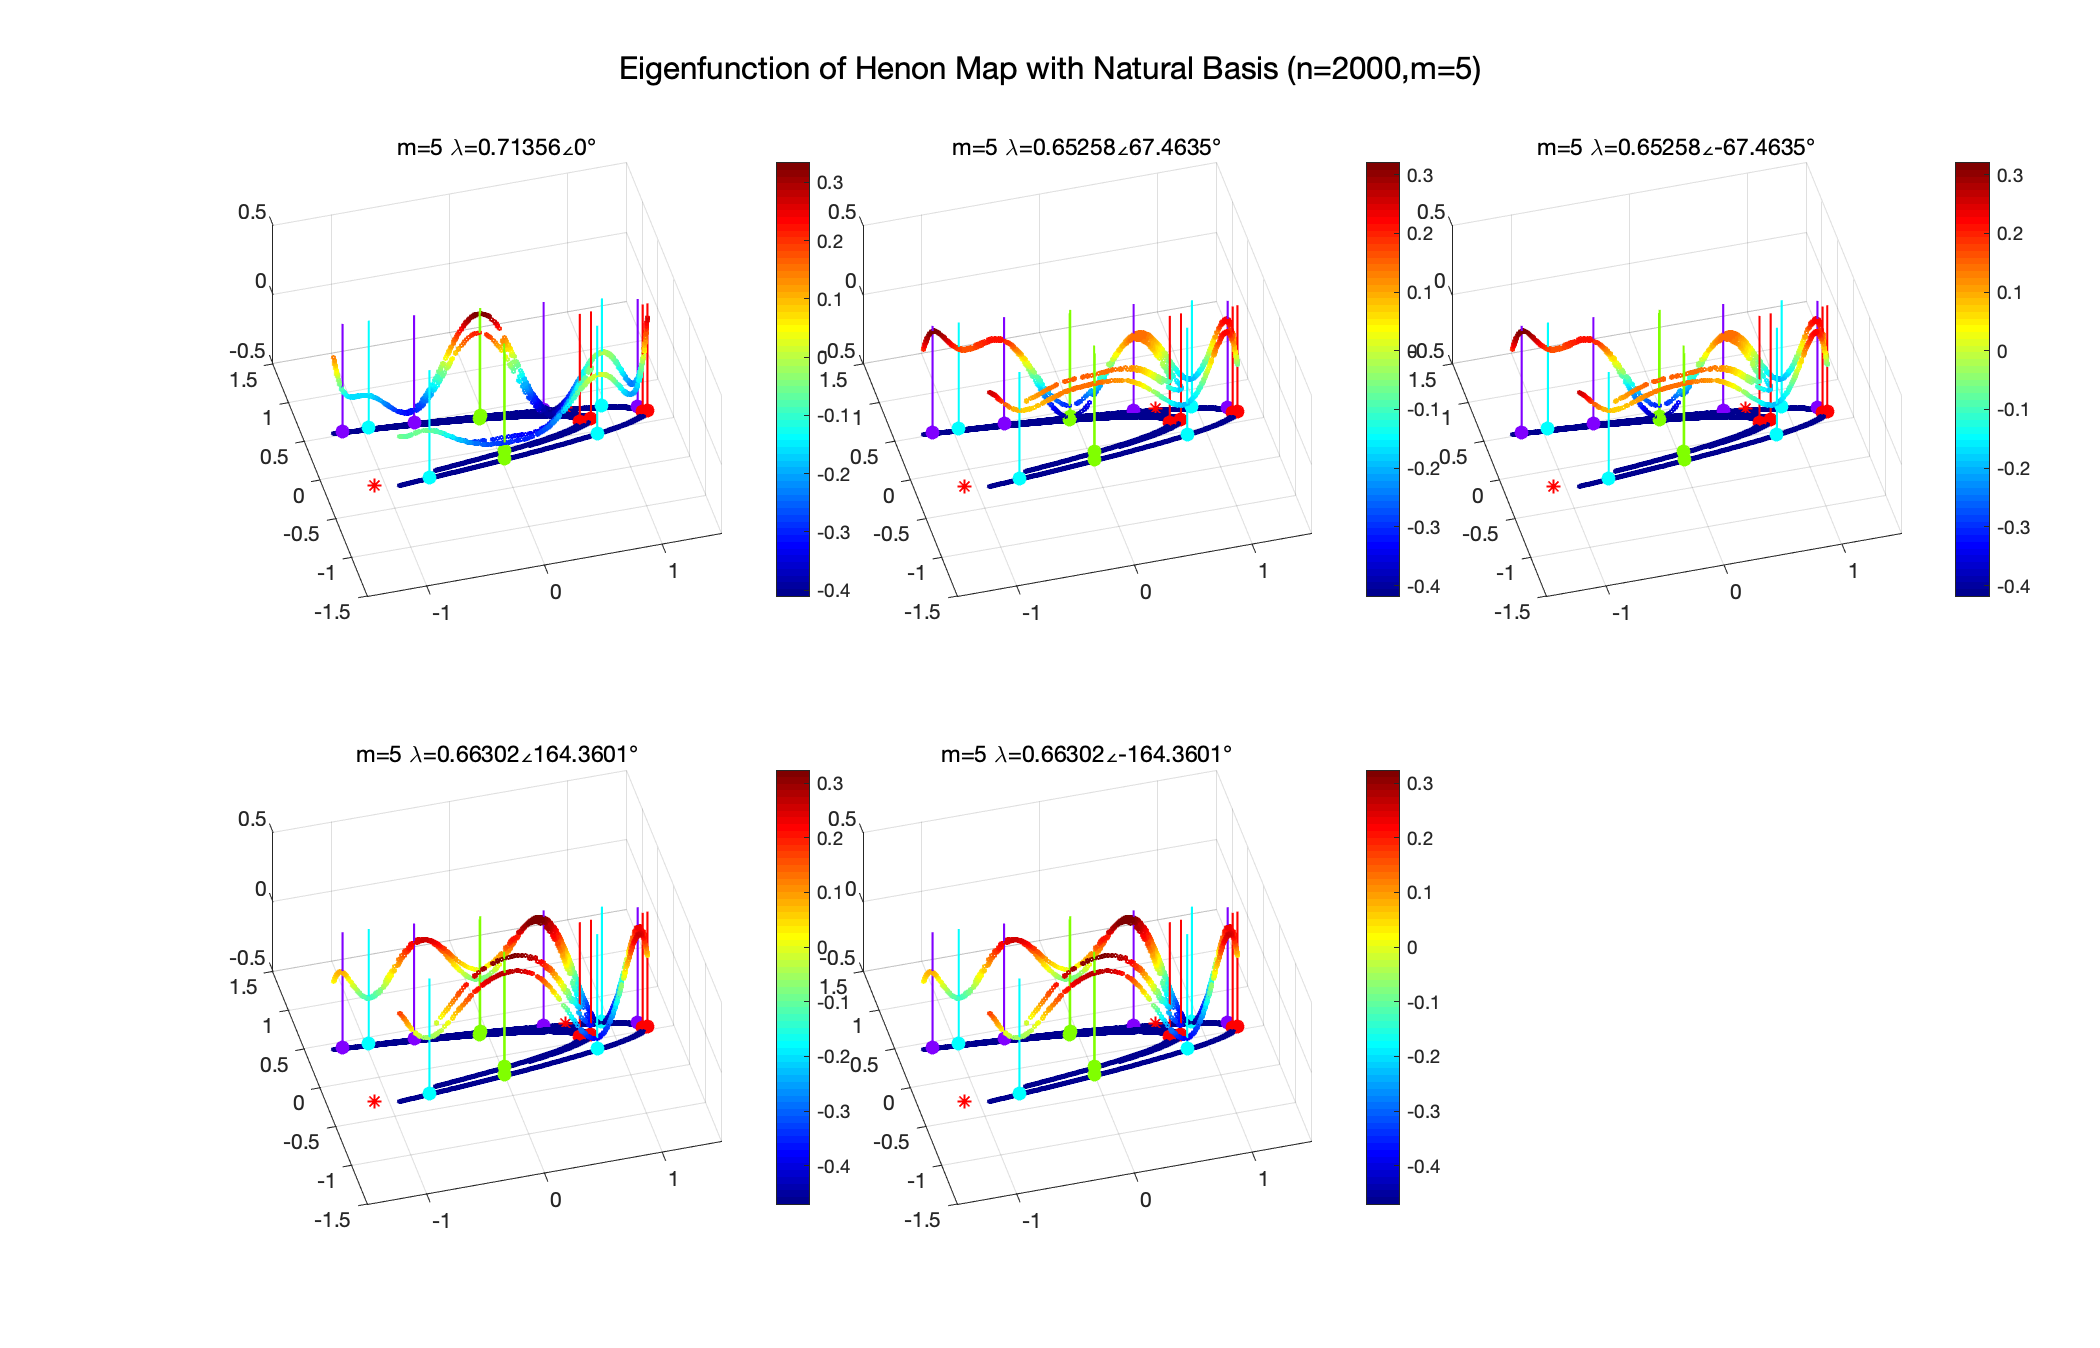
\includegraphics[scale=0.2]{henon/attractors/Henon_eigen_natural_attr_n2000m5}}
    \subfloat[m=6]{
      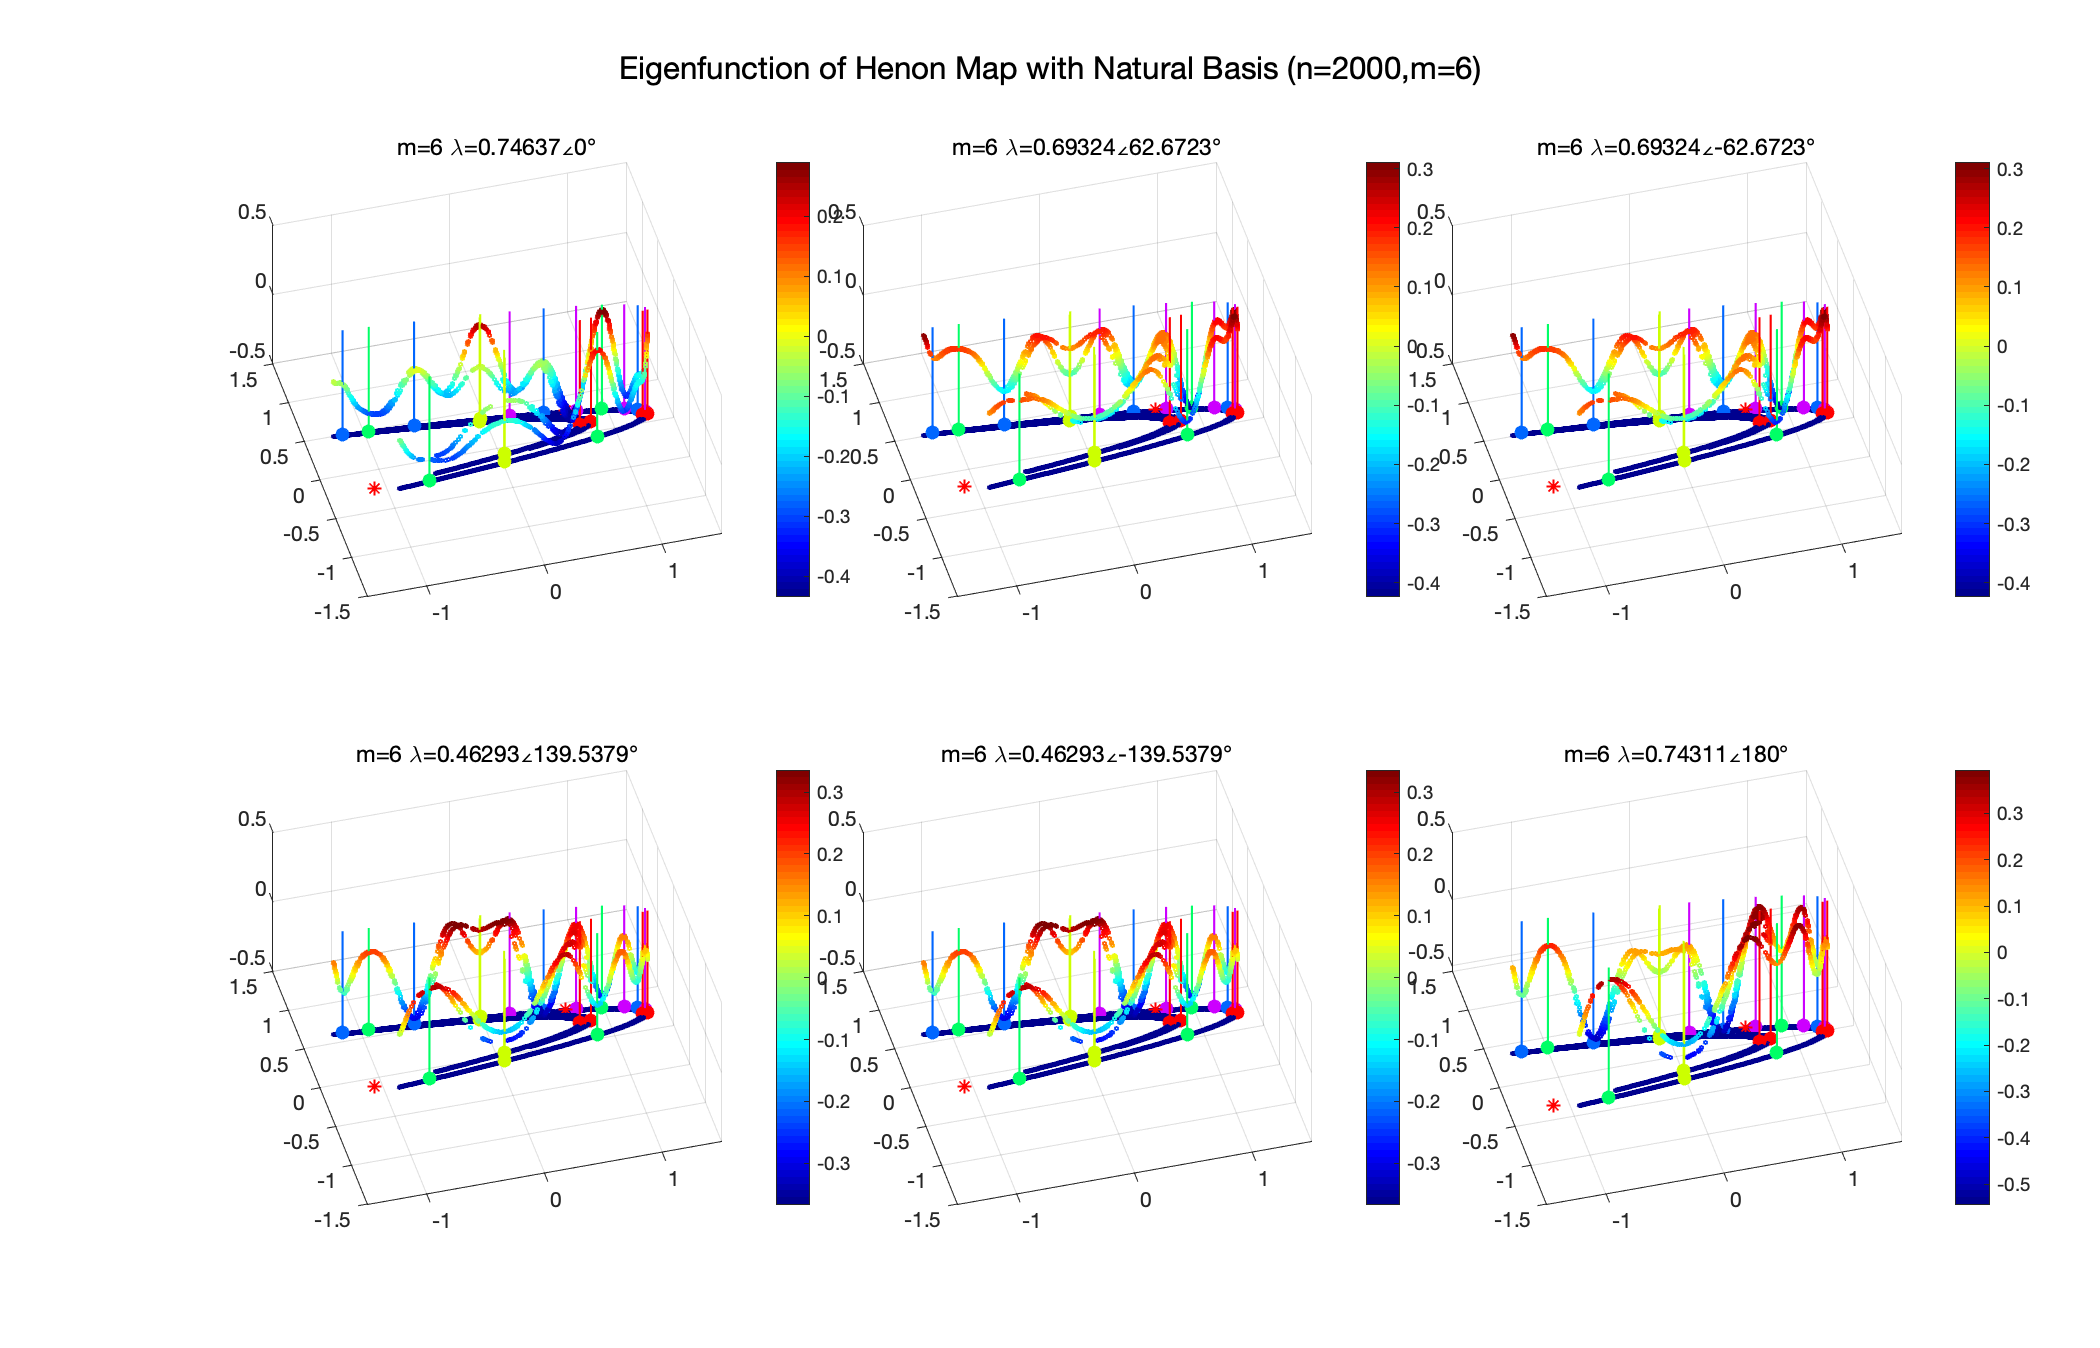
\includegraphics[scale=0.2]{henon/attractors/Henon_eigen_natural_attr_n2000m6}}
    \\
    \subfloat[m=7]{
      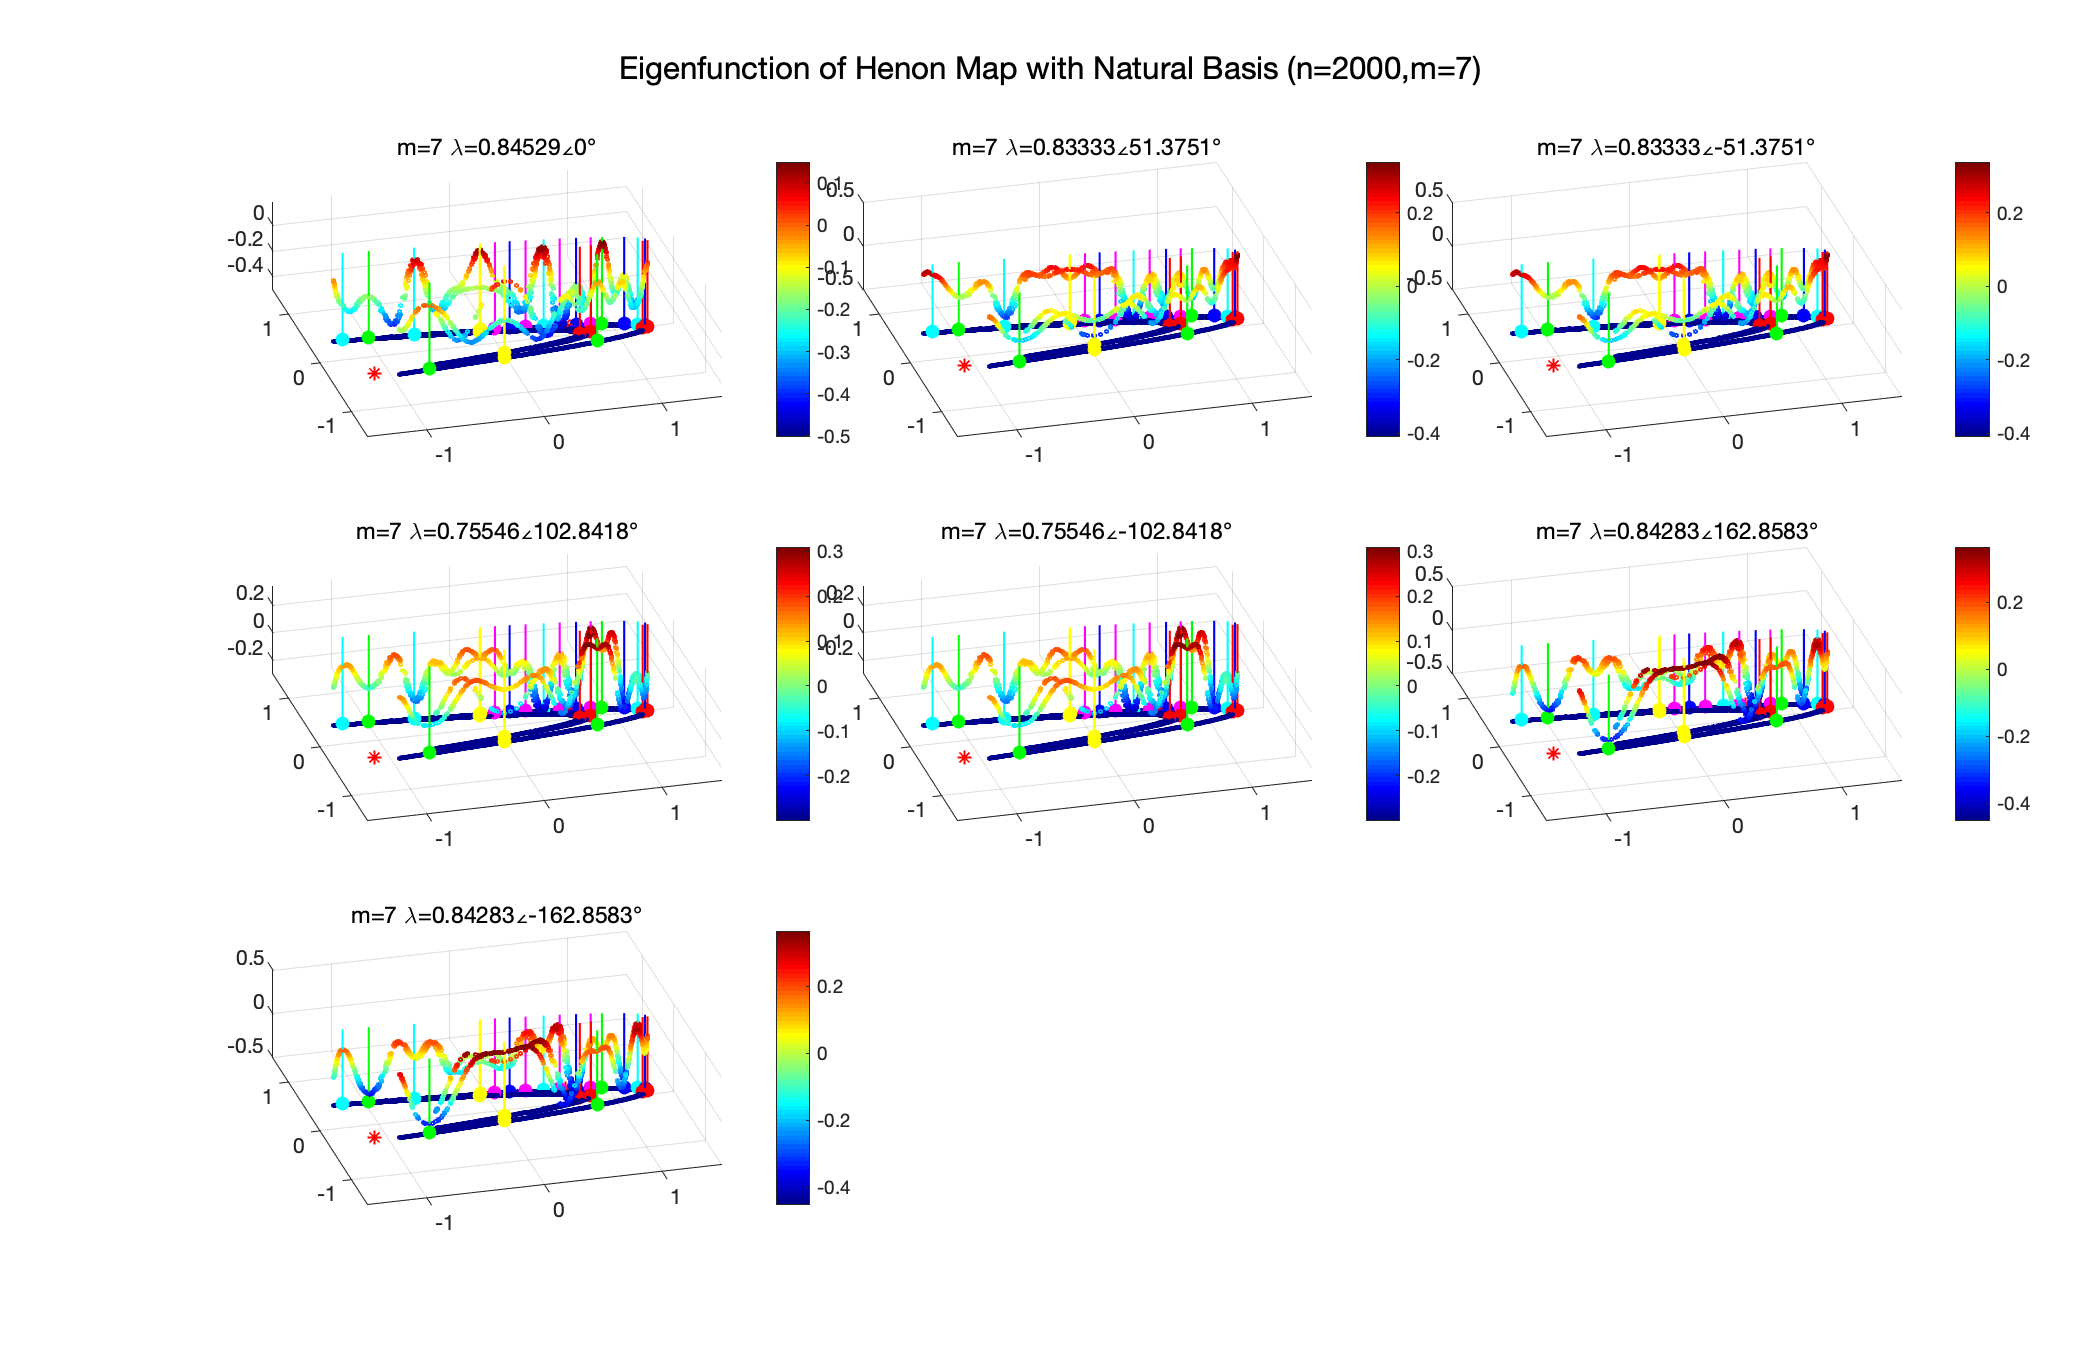
\includegraphics[scale=0.2]{henon/attractors/Henon_eigen_natural_attr_n2000m7}}
    \subfloat[m=8]{
      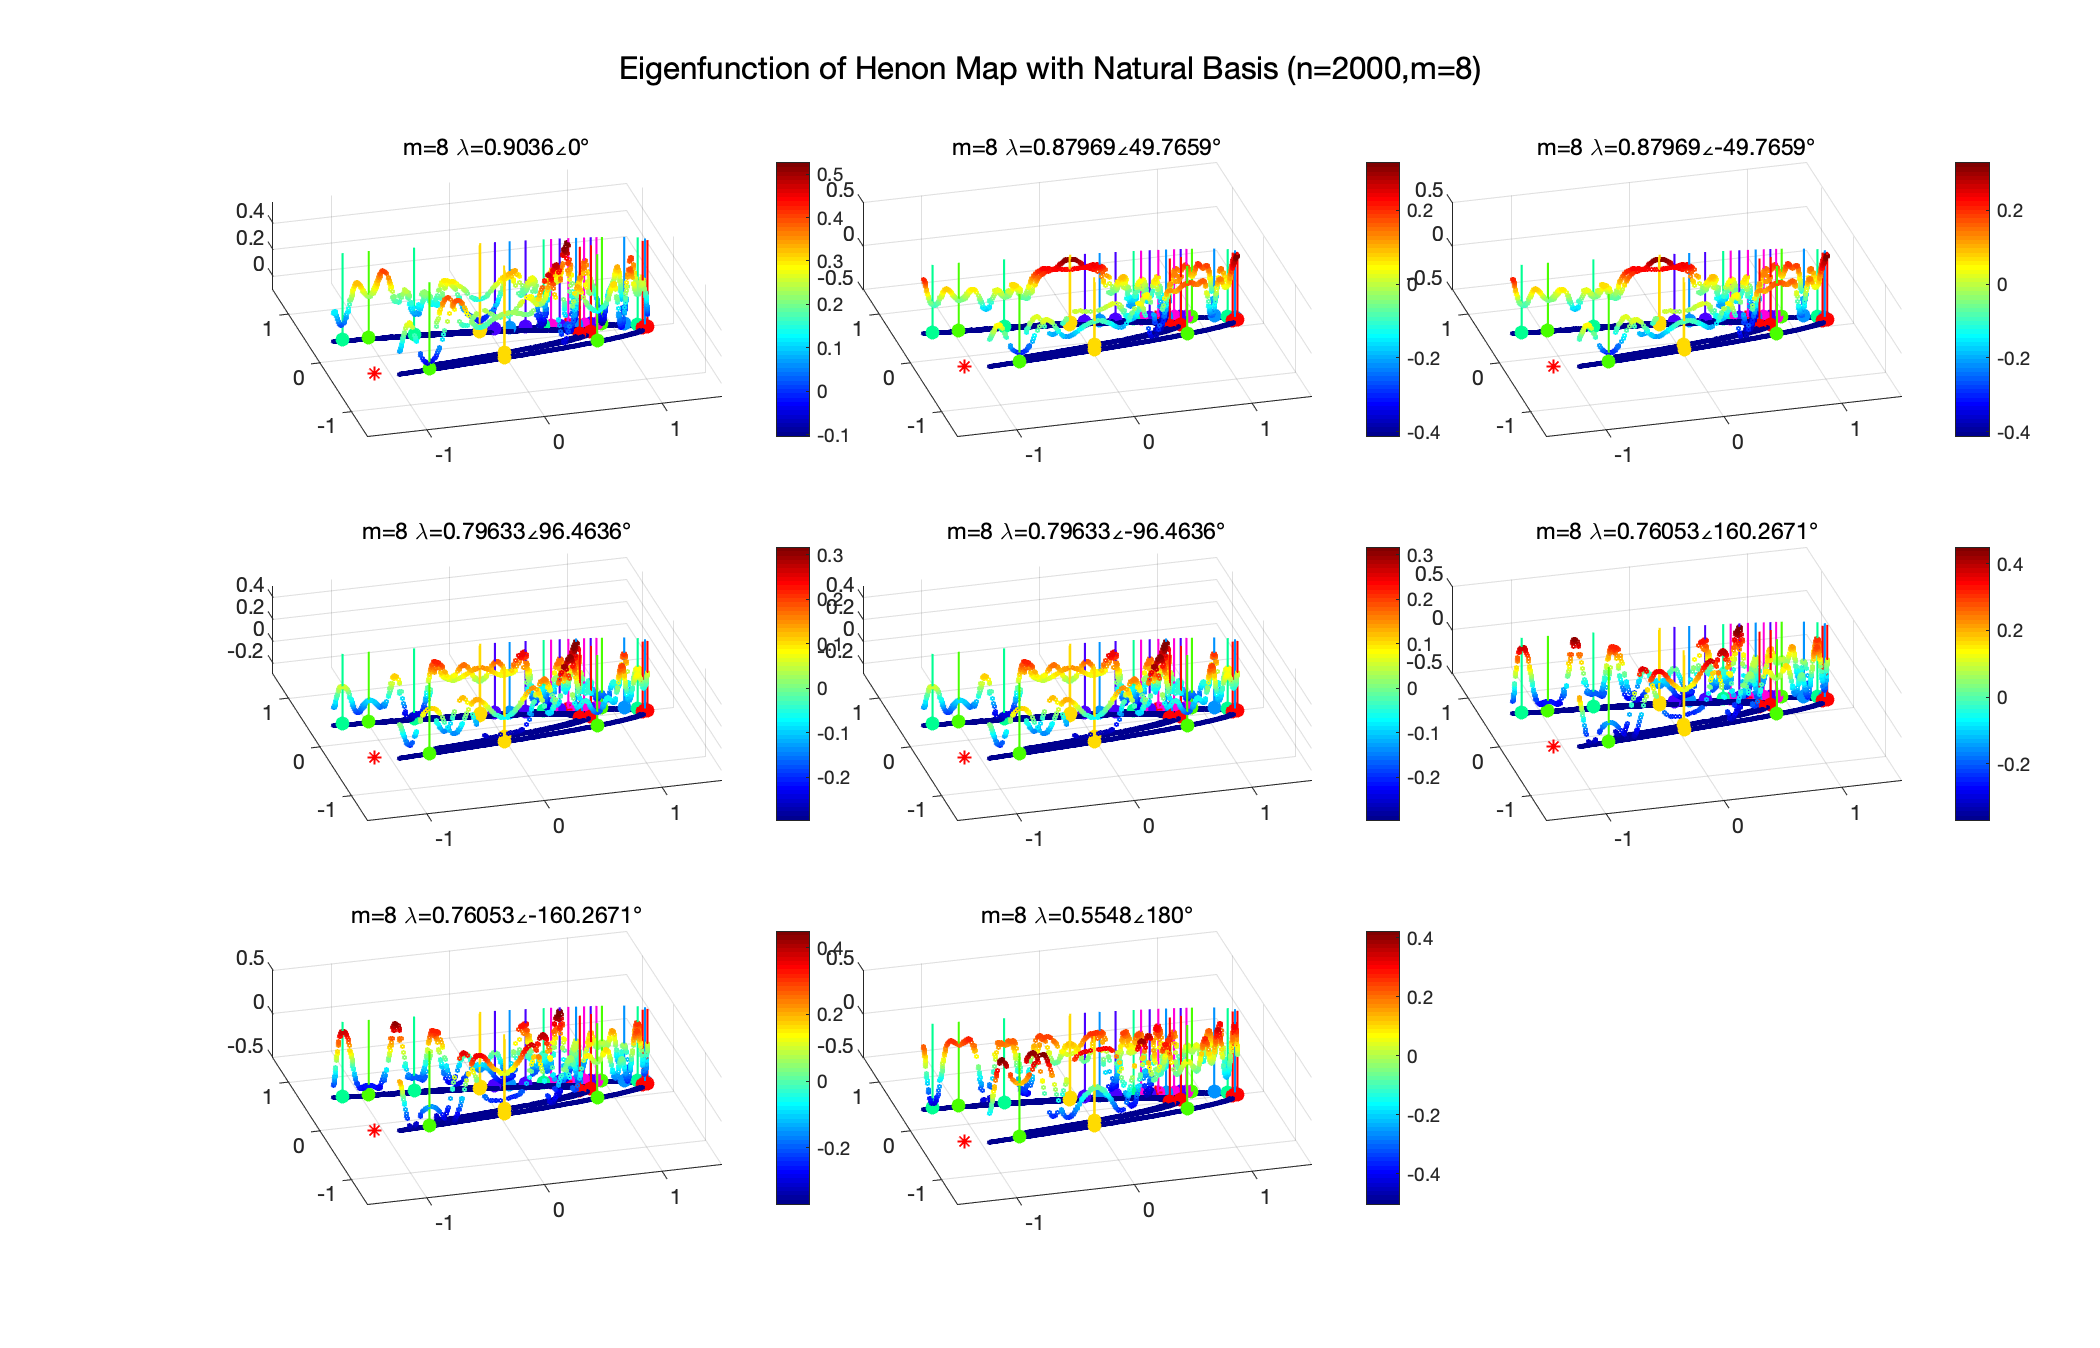
\includegraphics[scale=0.2]{henon/attractors/Henon_eigen_natural_attr_n2000m8}}
    \\
    \caption{埃农映射的边界点与本征函数对吸引子的划分($n=2000$)}
\end{figure}

\begin{figure}
	\centering
	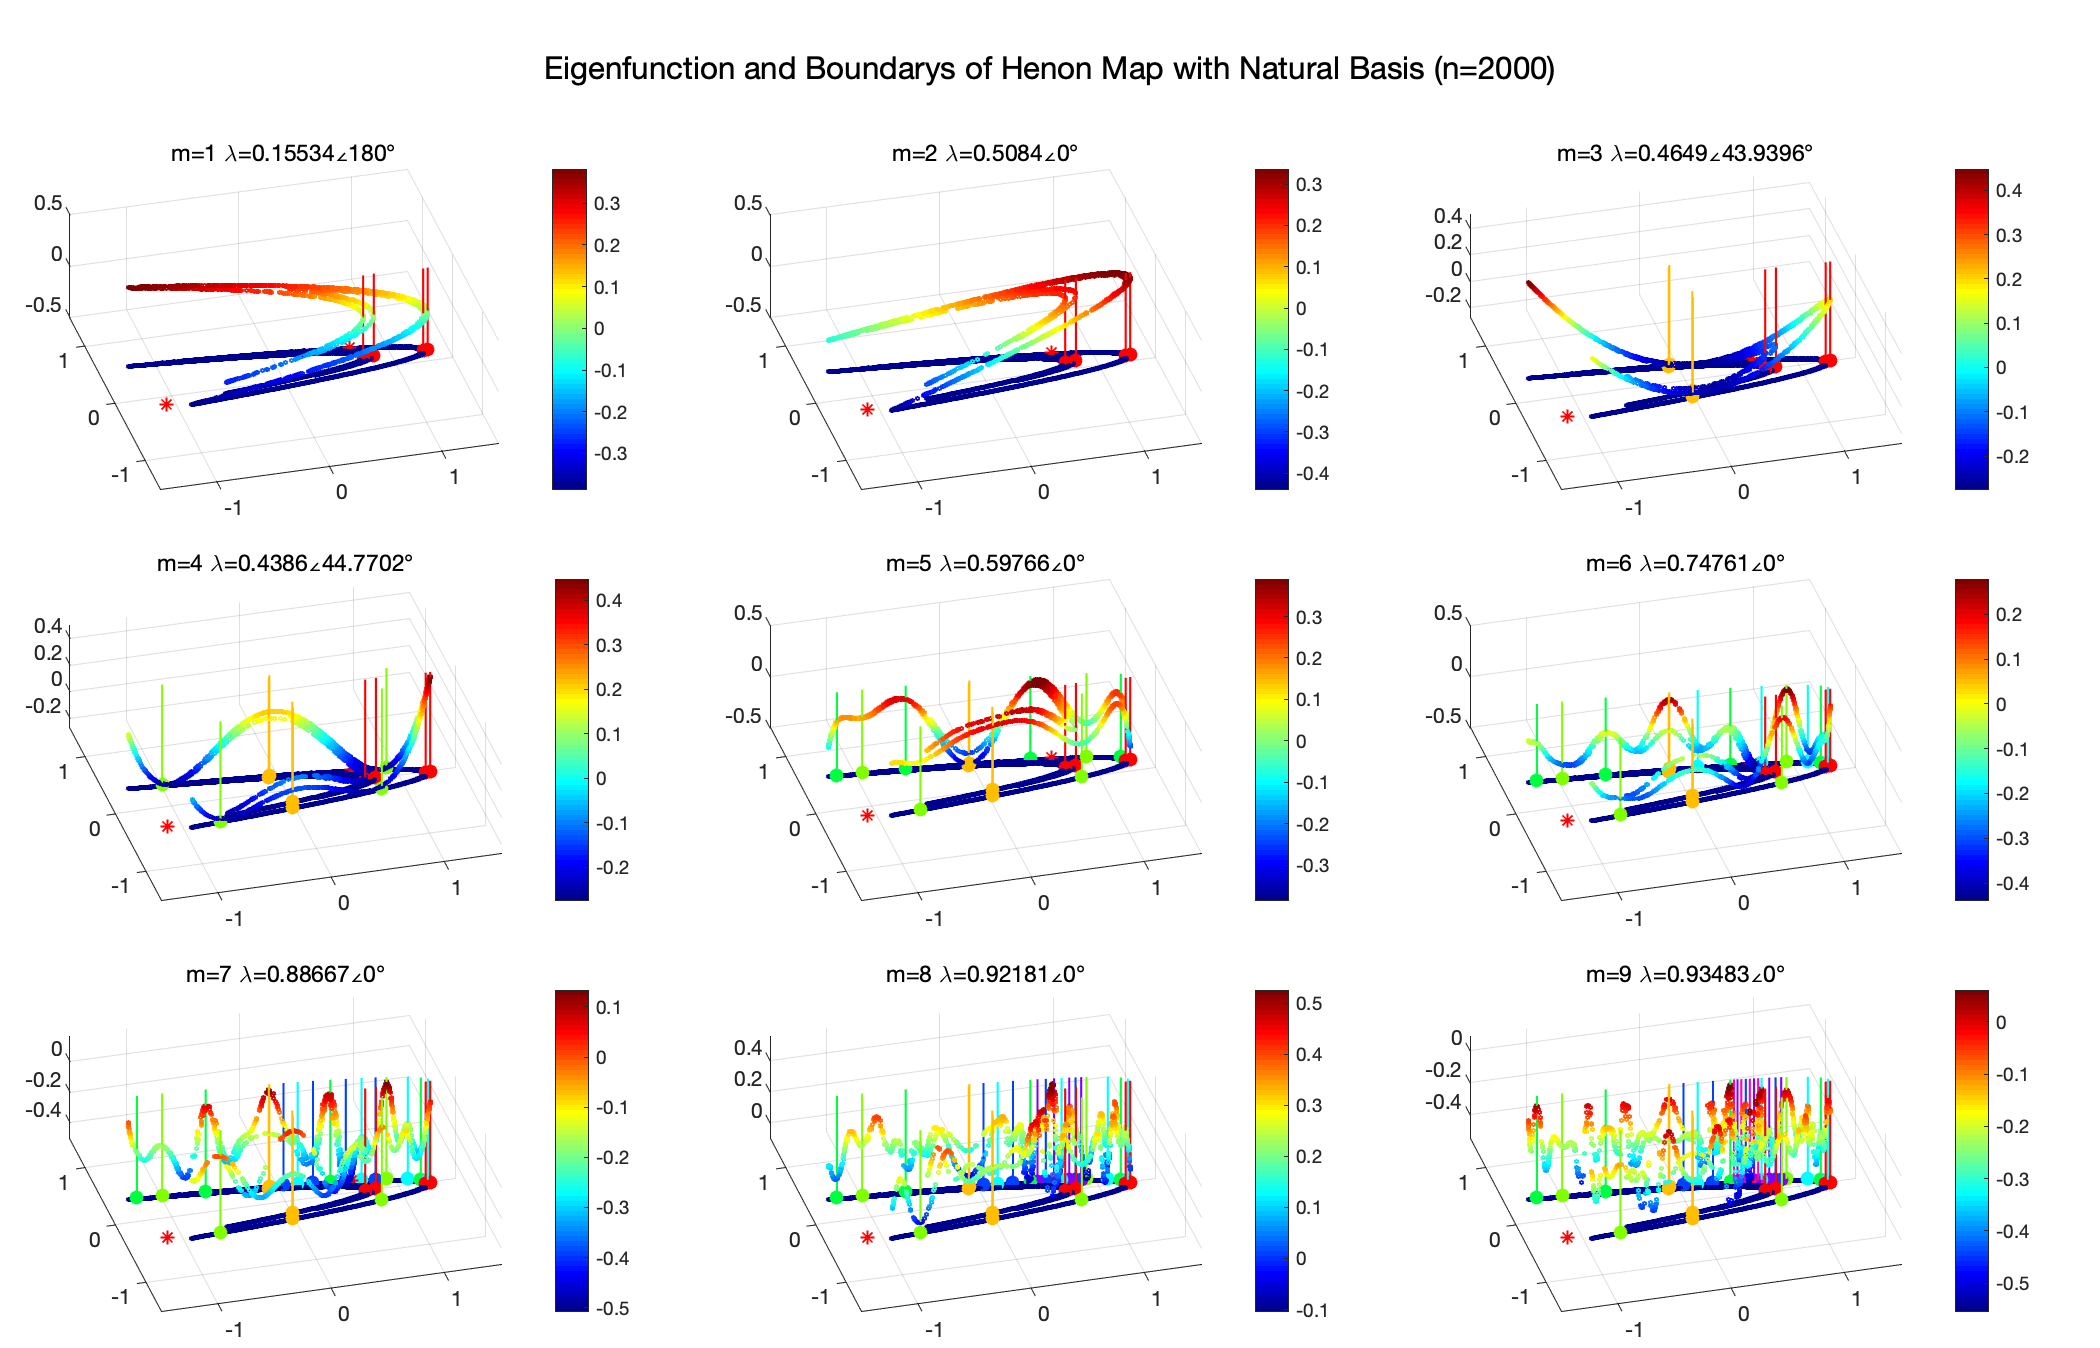
\includegraphics[scale=0.4]{henon/attractors/Henon_eigen_natural_attr_n2000}
    \caption{埃农映射的边界点与本征函数对吸引子的划分($n=2000$)}
\end{figure}

\subsubsection{埃农映射的周期轨道}
\begin{figure}
	\centering
	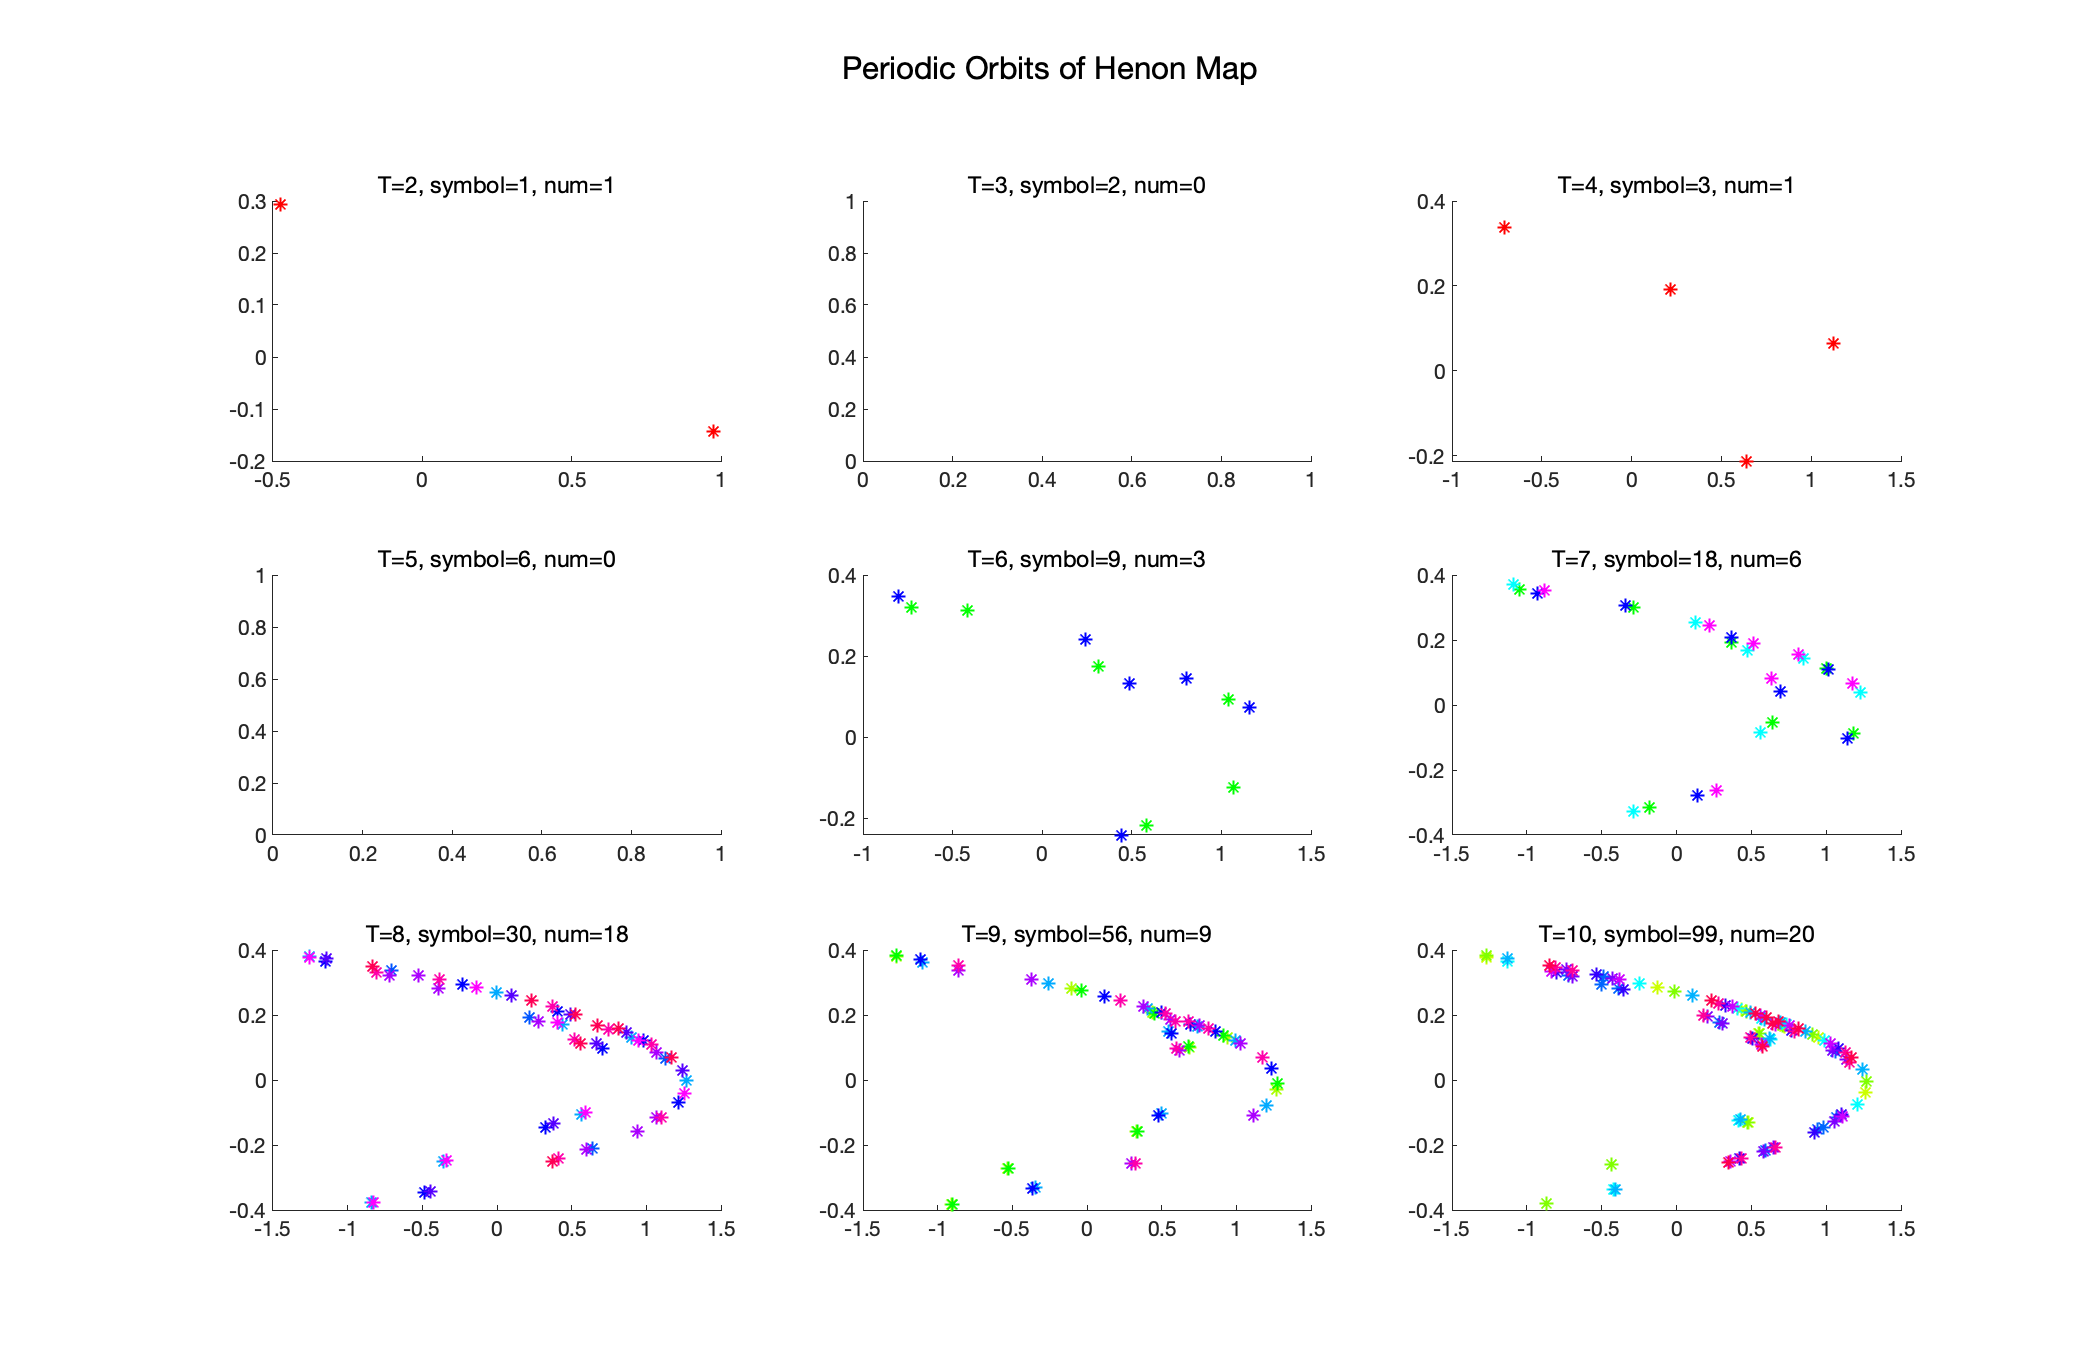
\includegraphics[scale=0.4]{henon/period/Henon_periodic_orbits}
    \caption{埃农映射的周期轨道}
\end{figure}

\begin{figure}
    \centering
    \subfloat[T=2]{
      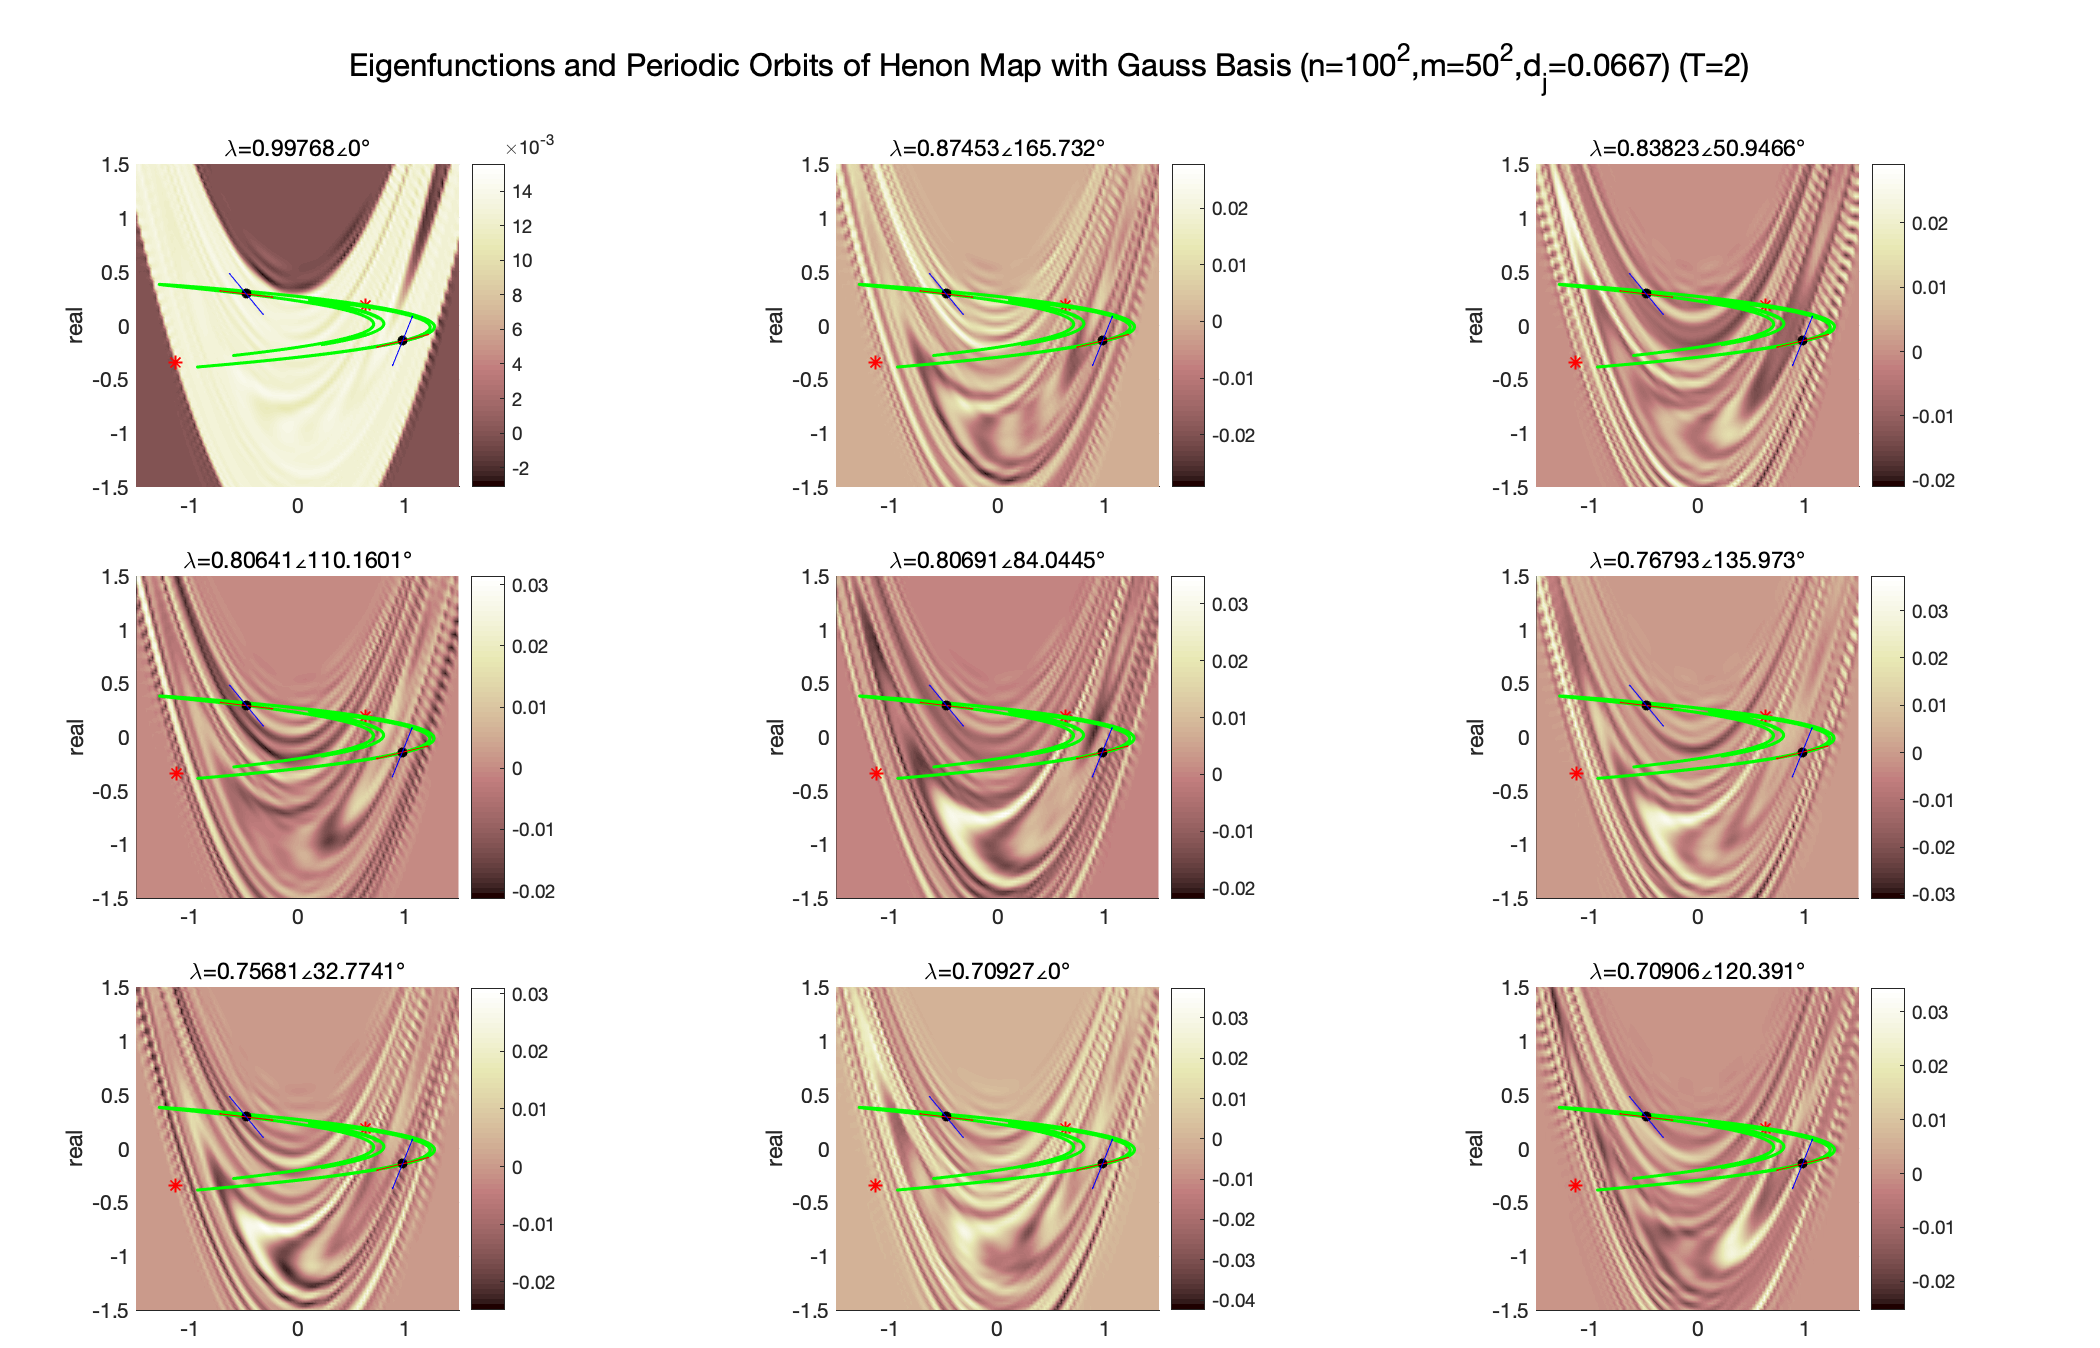
\includegraphics[scale=0.2]{henon/period/Henon_eigen_Gauss_period_n100m50T2}}
    \subfloat[T=4]{
      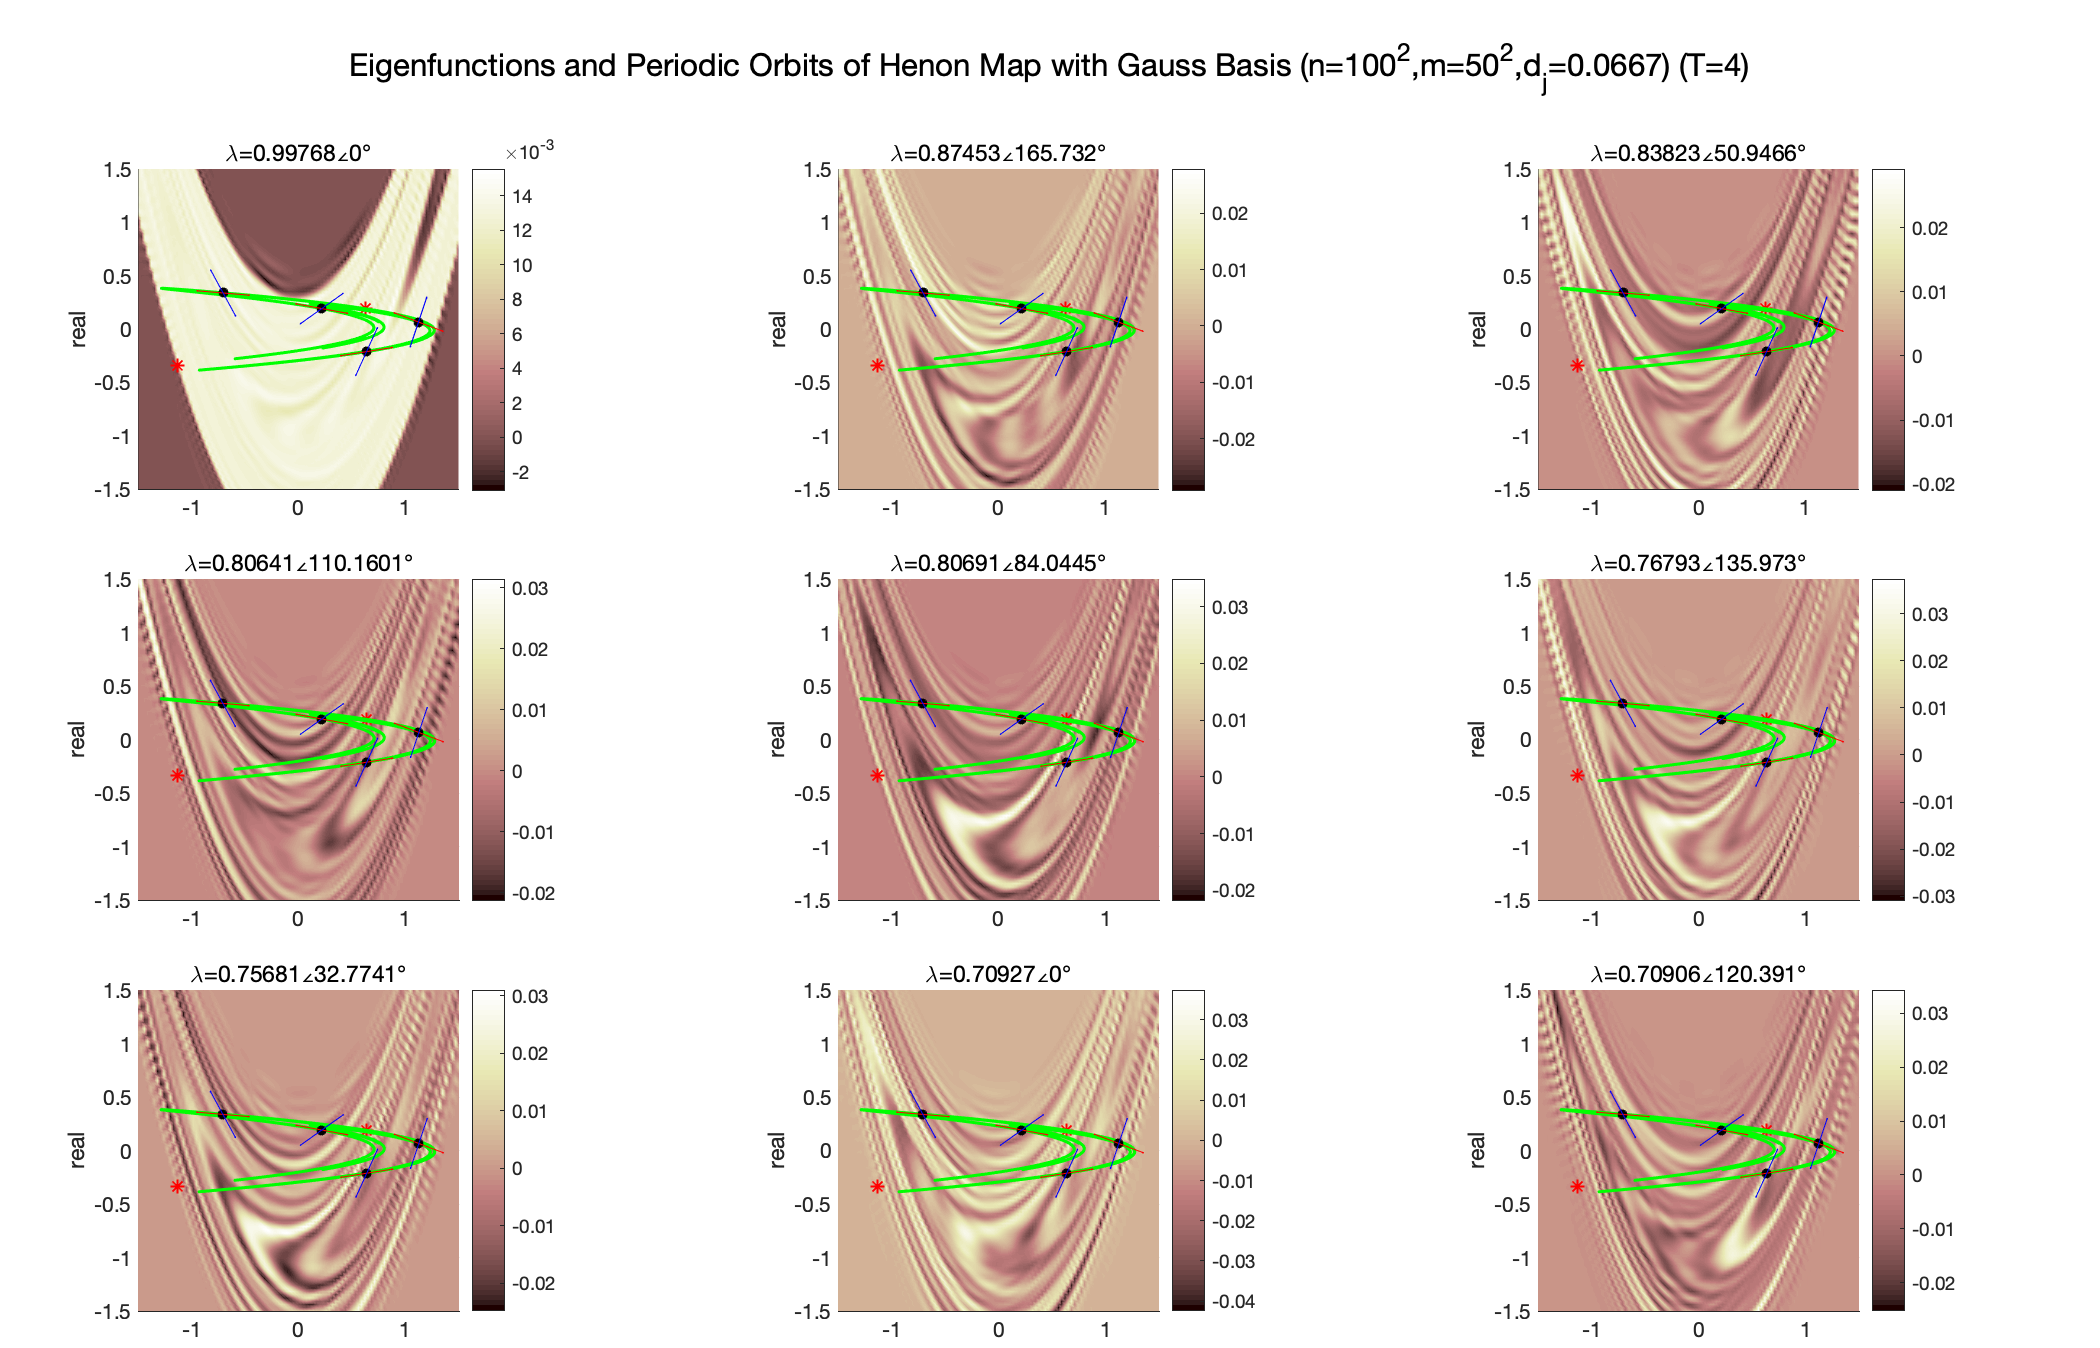
\includegraphics[scale=0.2]{henon/period/Henon_eigen_Gauss_period_n100m50T4}}
    \\
    \subfloat[T=6]{
      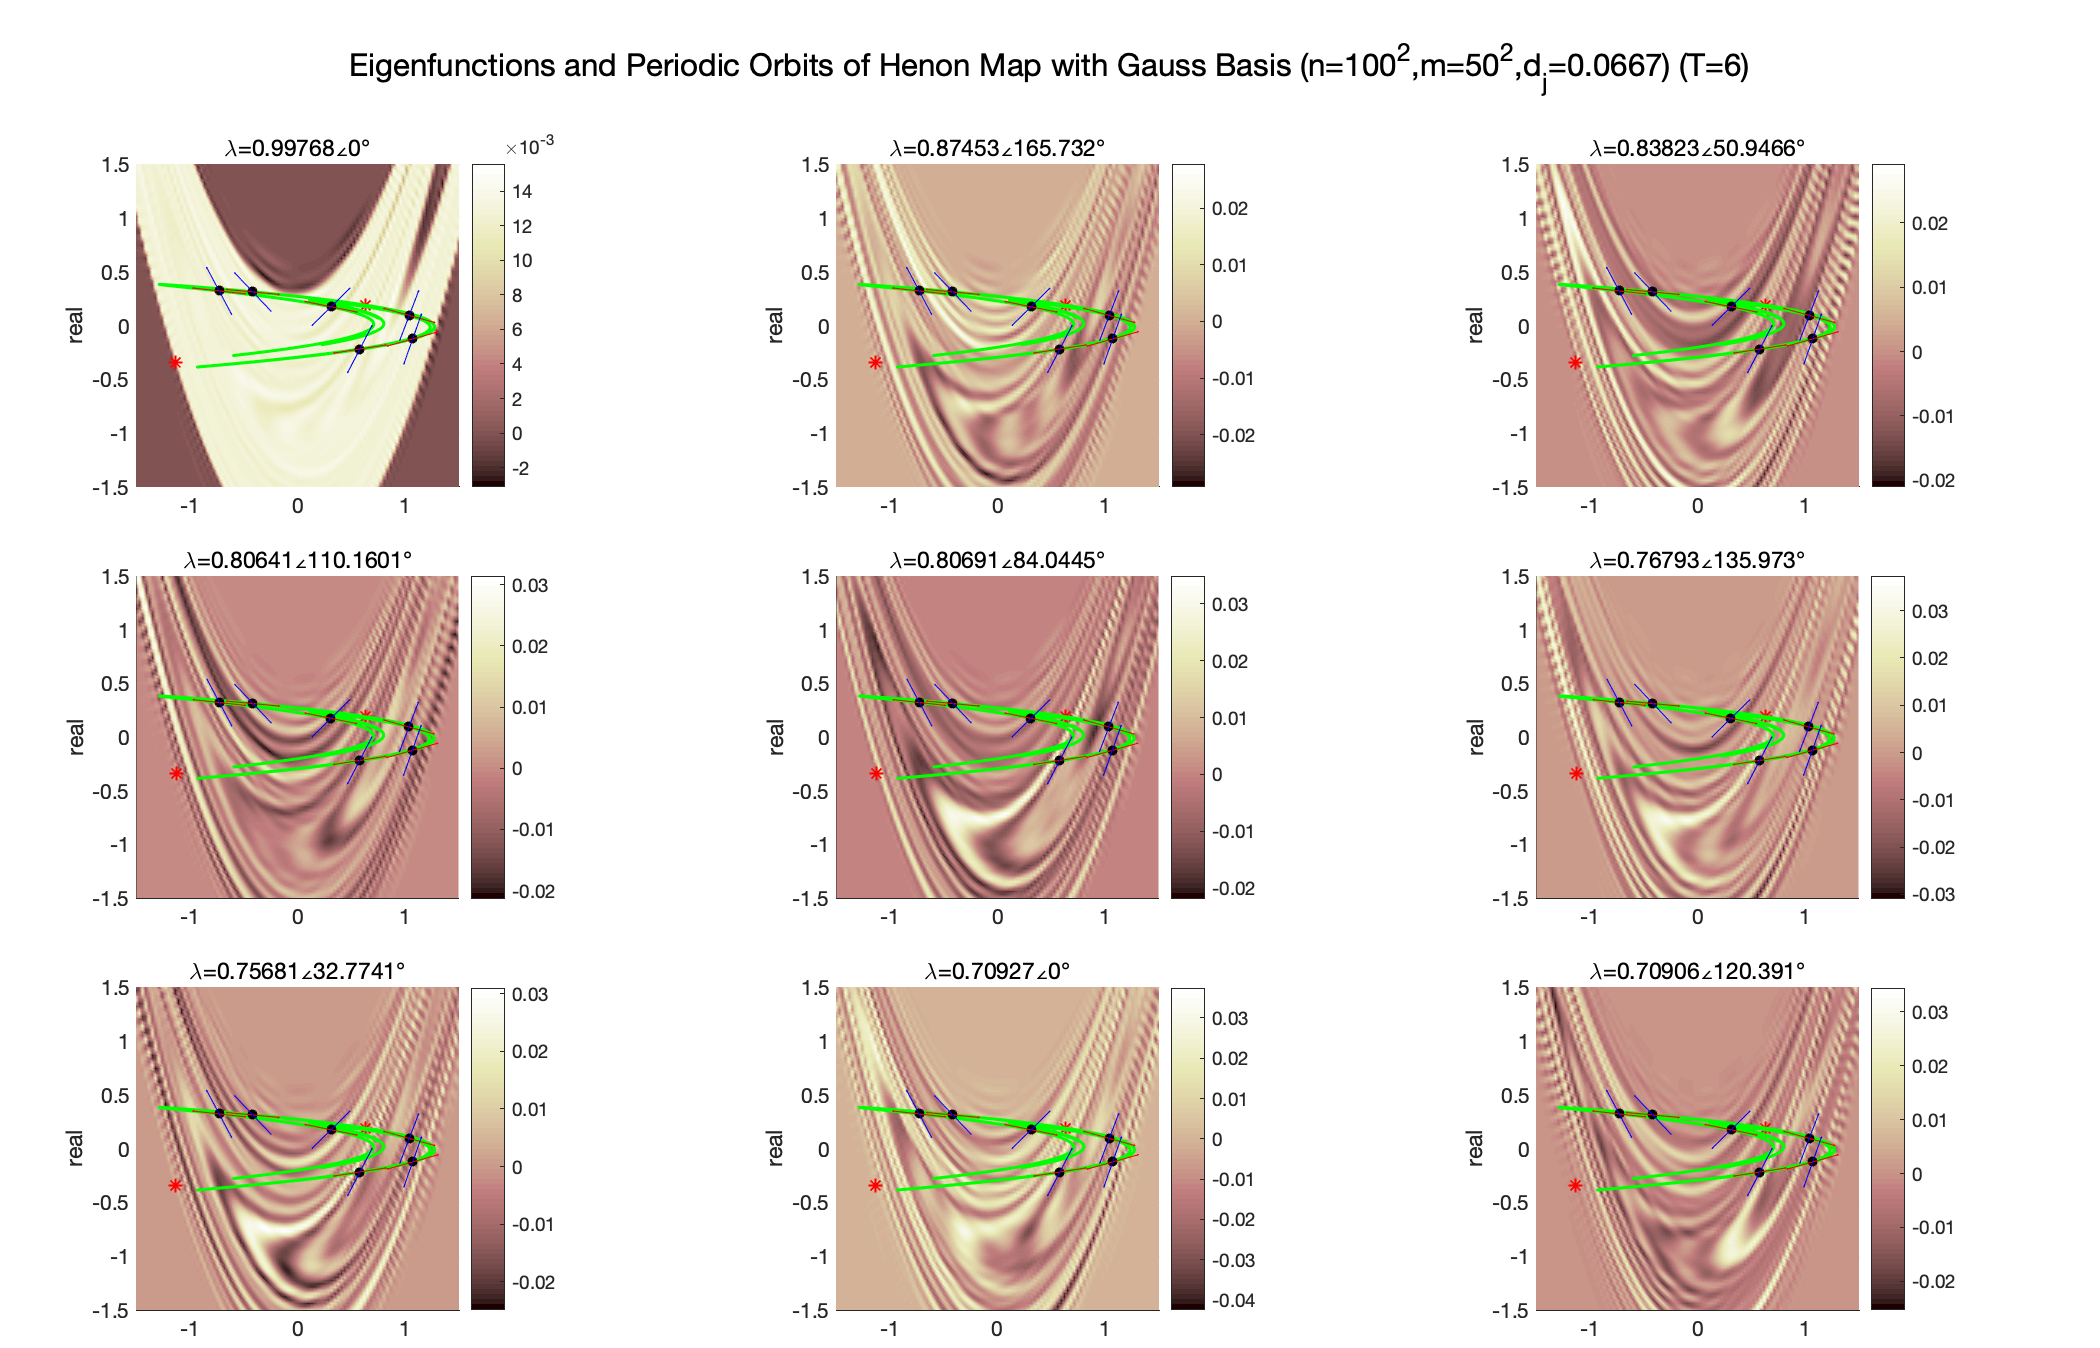
\includegraphics[scale=0.2]{henon/period/Henon_eigen_Gauss_period_n100m50T6}}
    \subfloat[T=7]{
      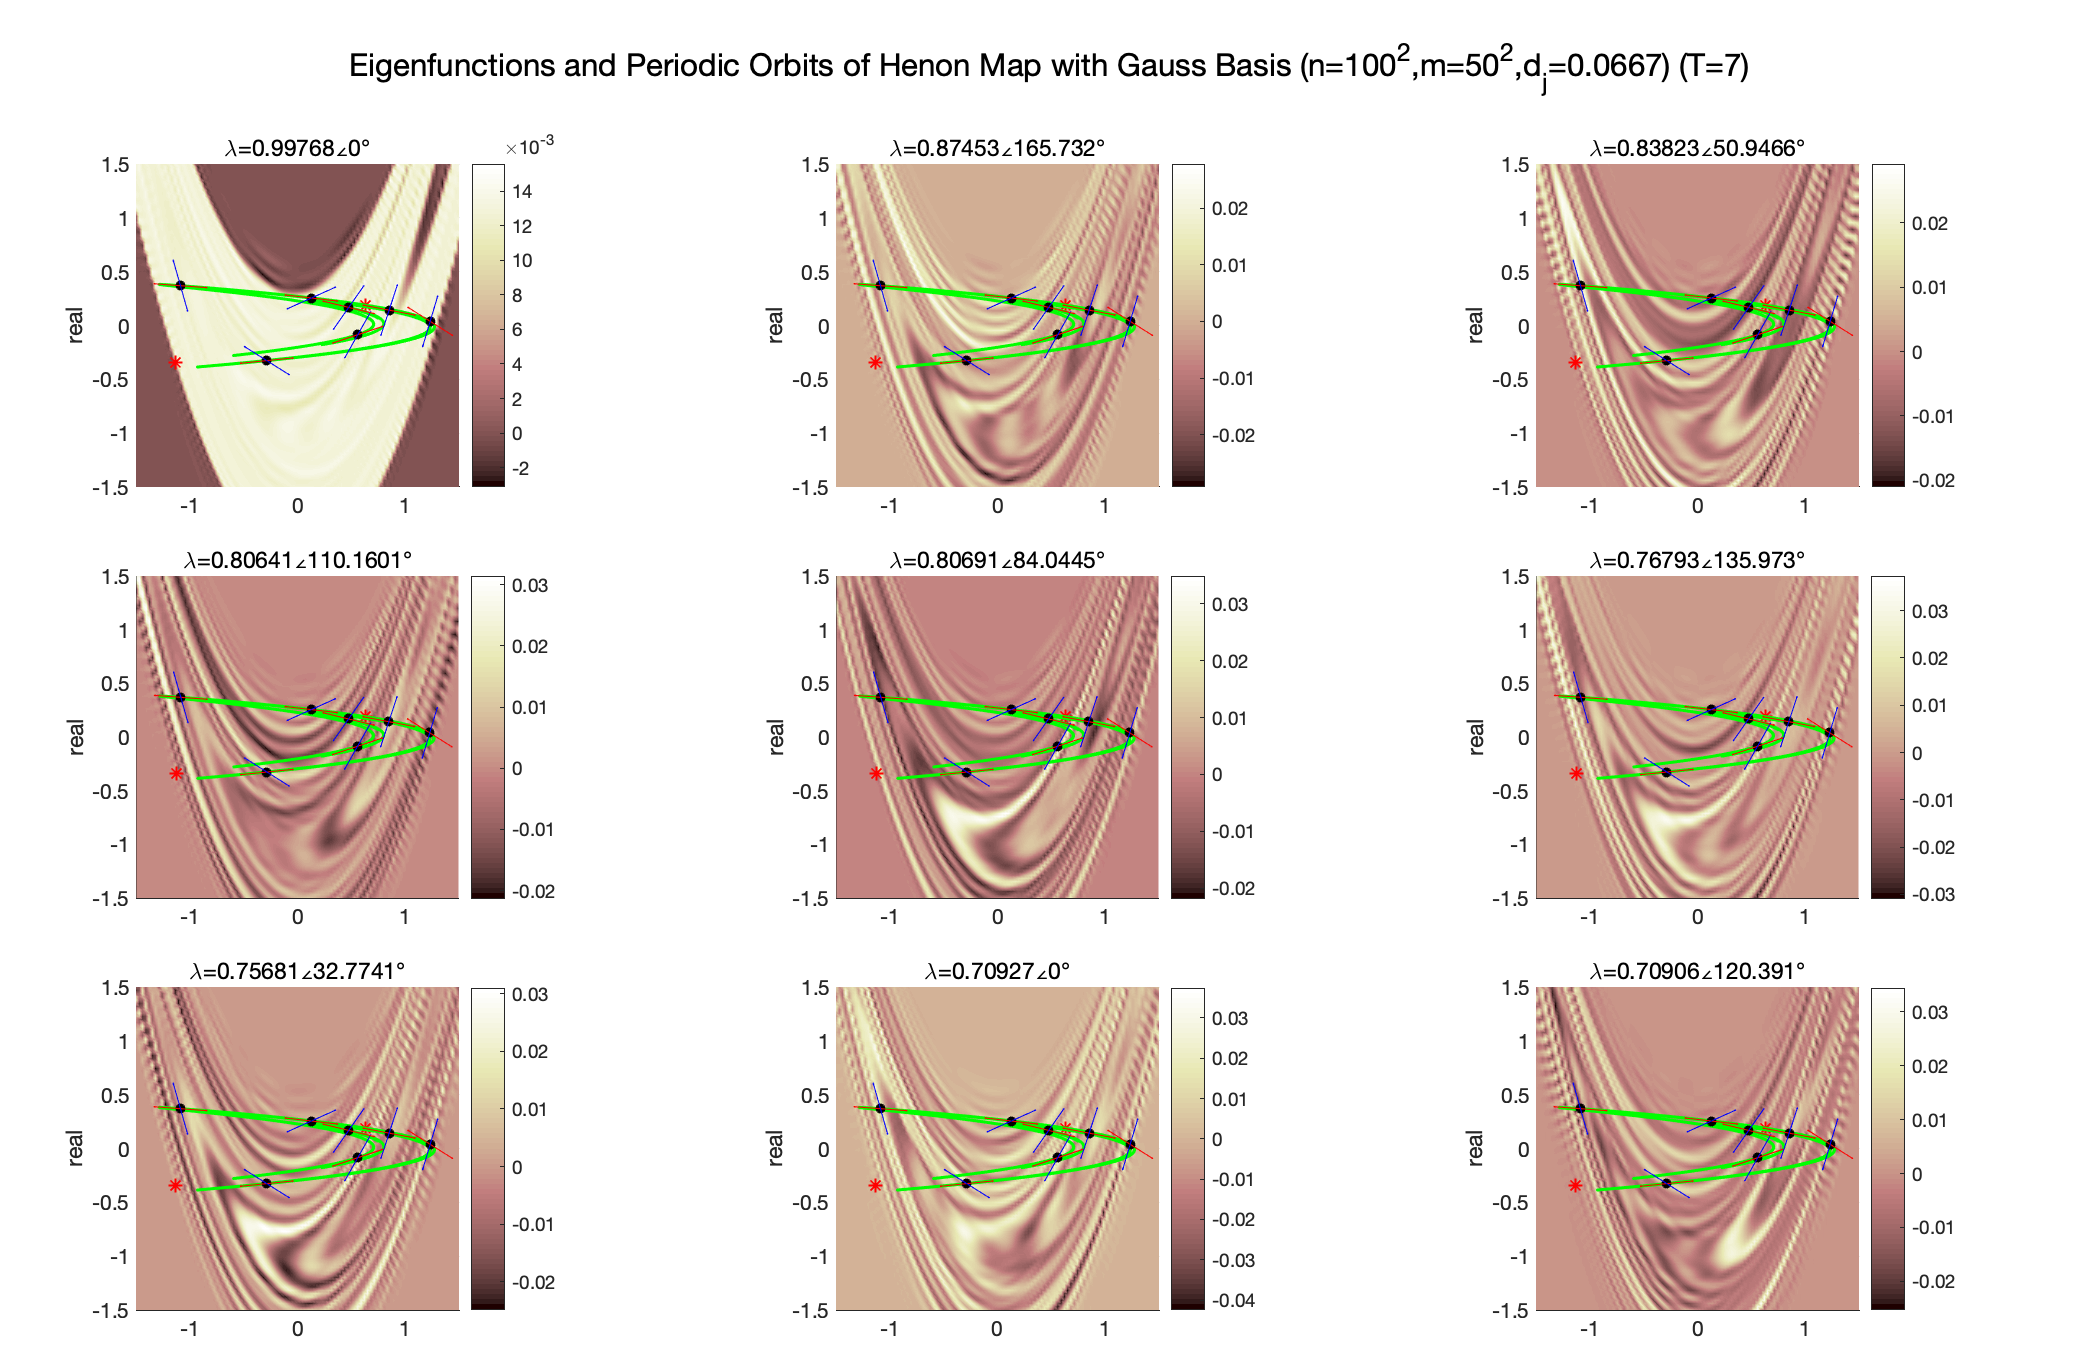
\includegraphics[scale=0.2]{henon/period/Henon_eigen_Gauss_period_n100m50T7}}
    \\
    \caption{埃农映射的本征函数与周期轨道($n=100^2$,$m=50^2,d_j=\frac{3}{45}$)}
\end{figure}

\begin{figure}
	\centering
	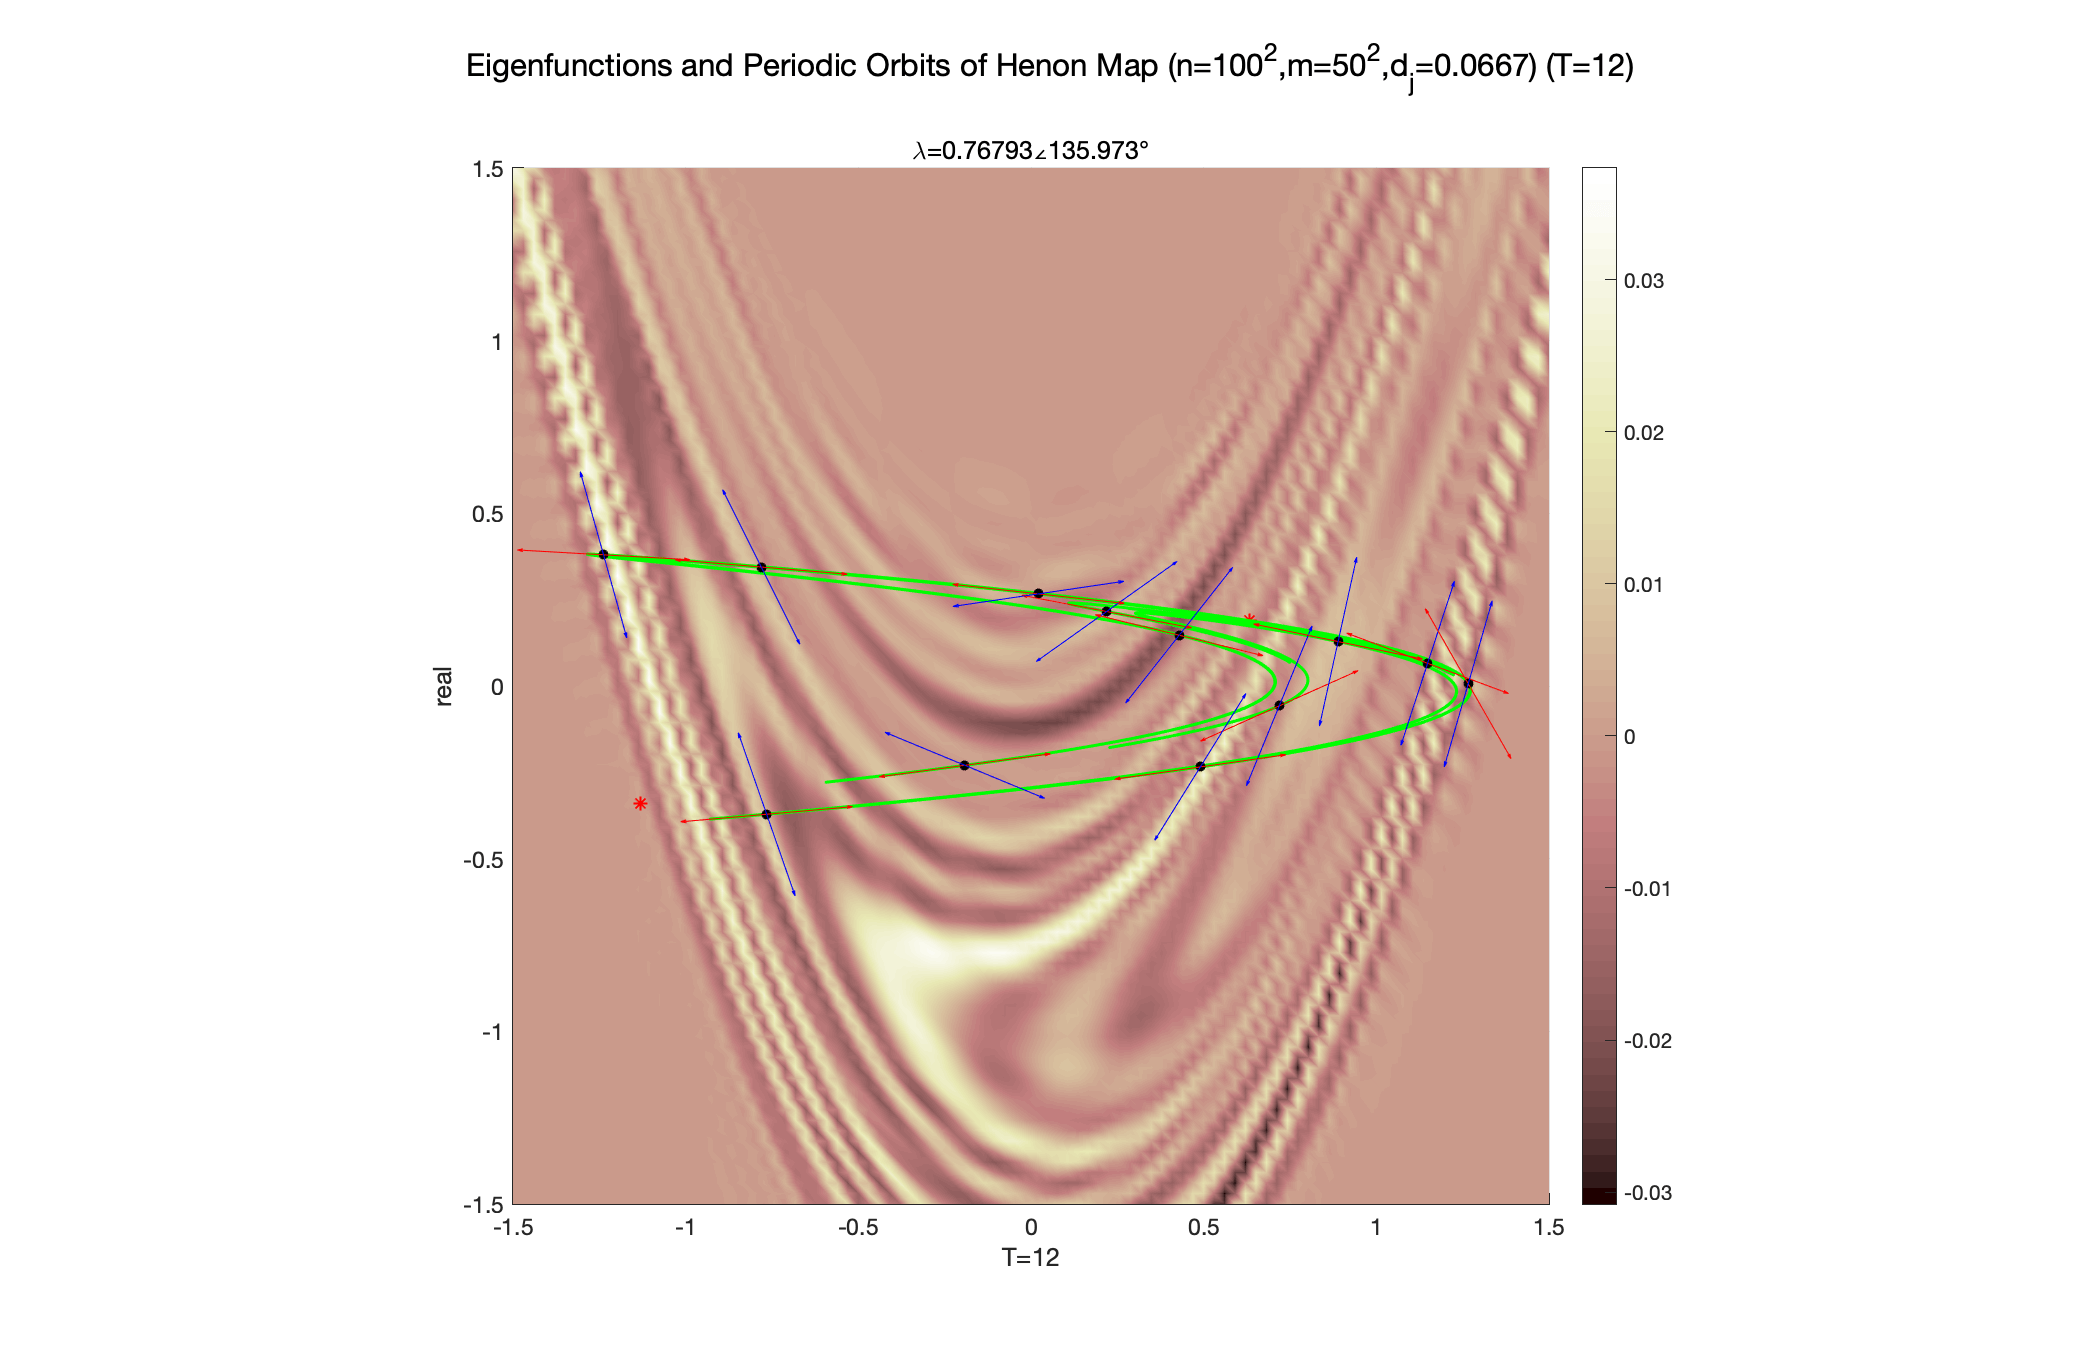
\includegraphics[scale=0.4]{henon/period/Henon_eigen_Gauss_period1_n100m50T12}
    \caption{埃农映射的本征函数与周期轨道(T=12)}
\end{figure}


\subsubsection{埃农映射的不稳定流型}

\begin{figure}
	\centering
	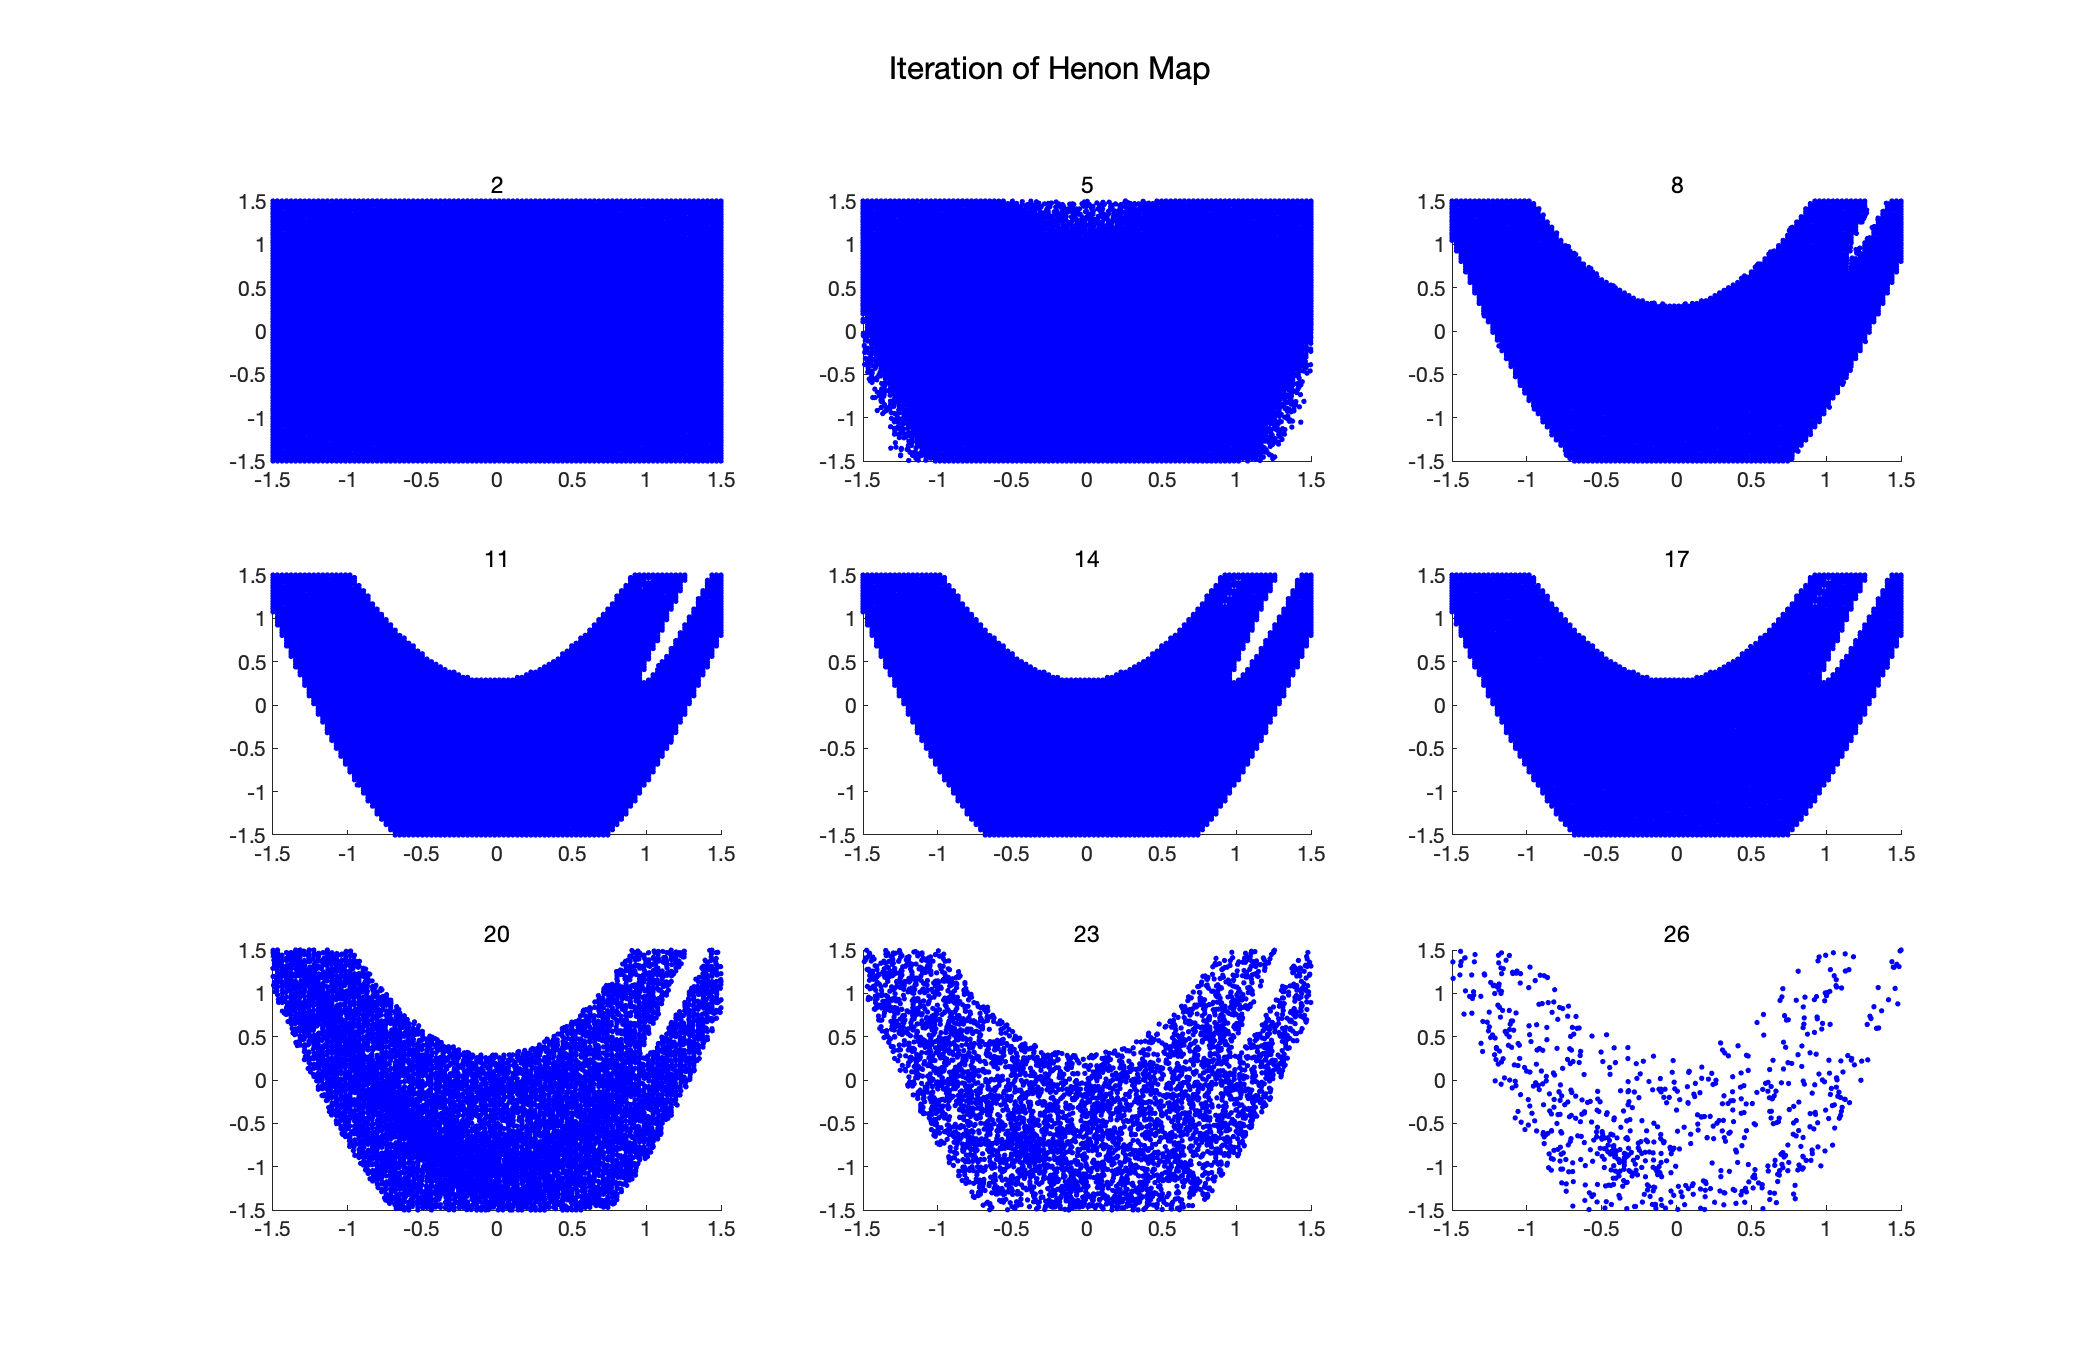
\includegraphics[scale=0.4]{henon/manifold/Henon_iter_reverse_forward}
    \caption{埃农映射的迭代}
\end{figure}
\begin{figure}
	\centering
	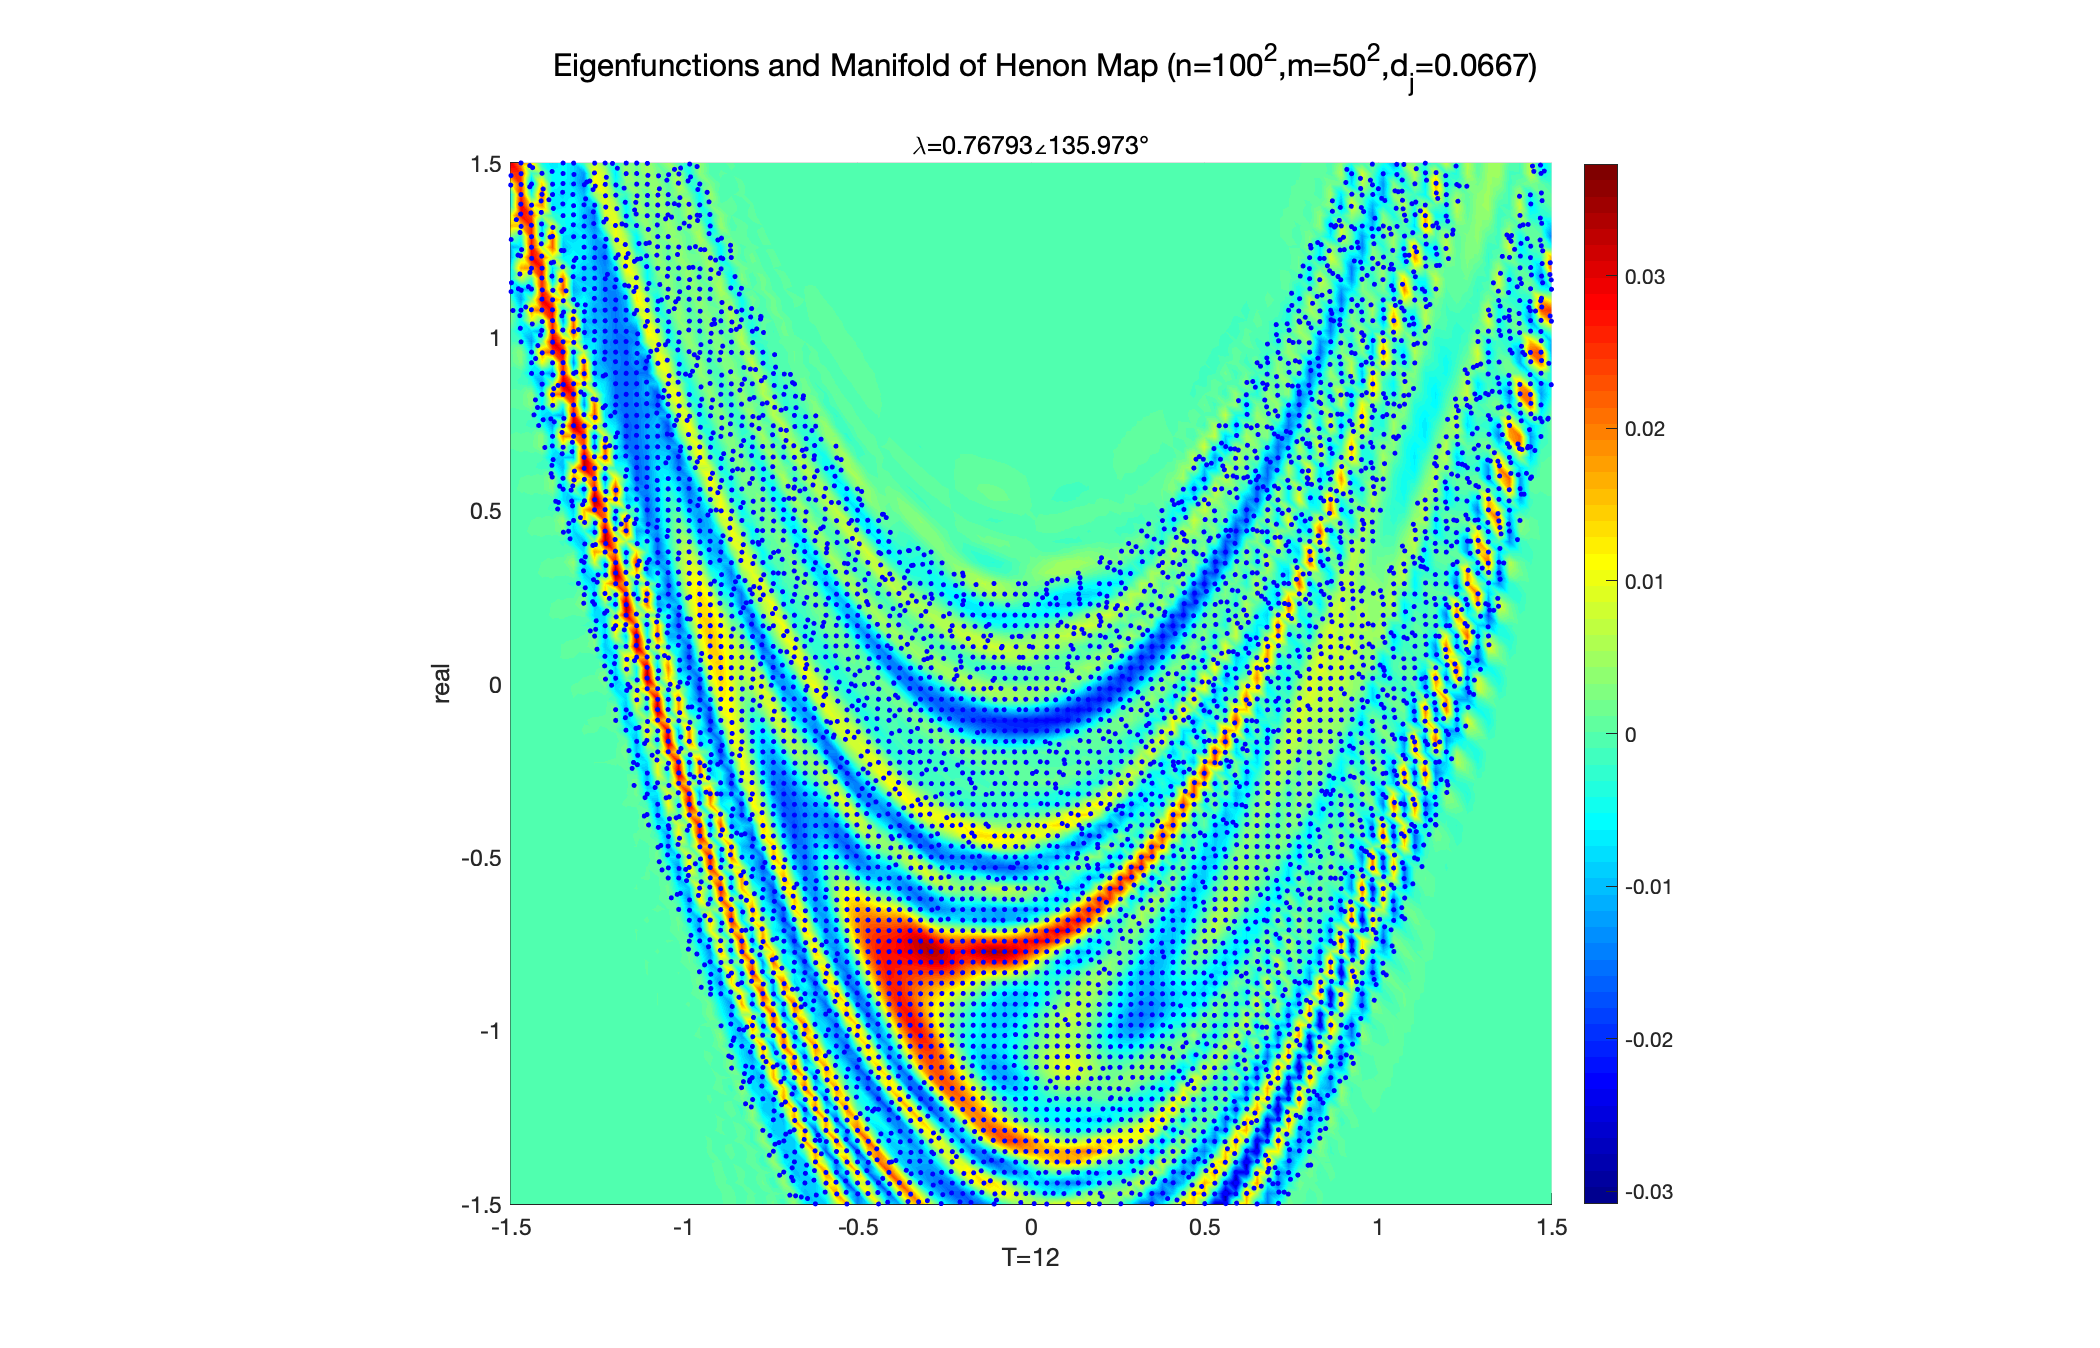
\includegraphics[scale=0.4]{henon/manifold/Henon_eigen_Gauss_manifold_n100m50}
    \caption{埃农映射的迭代与本征函数}
\end{figure}
\begin{figure}
	\centering
	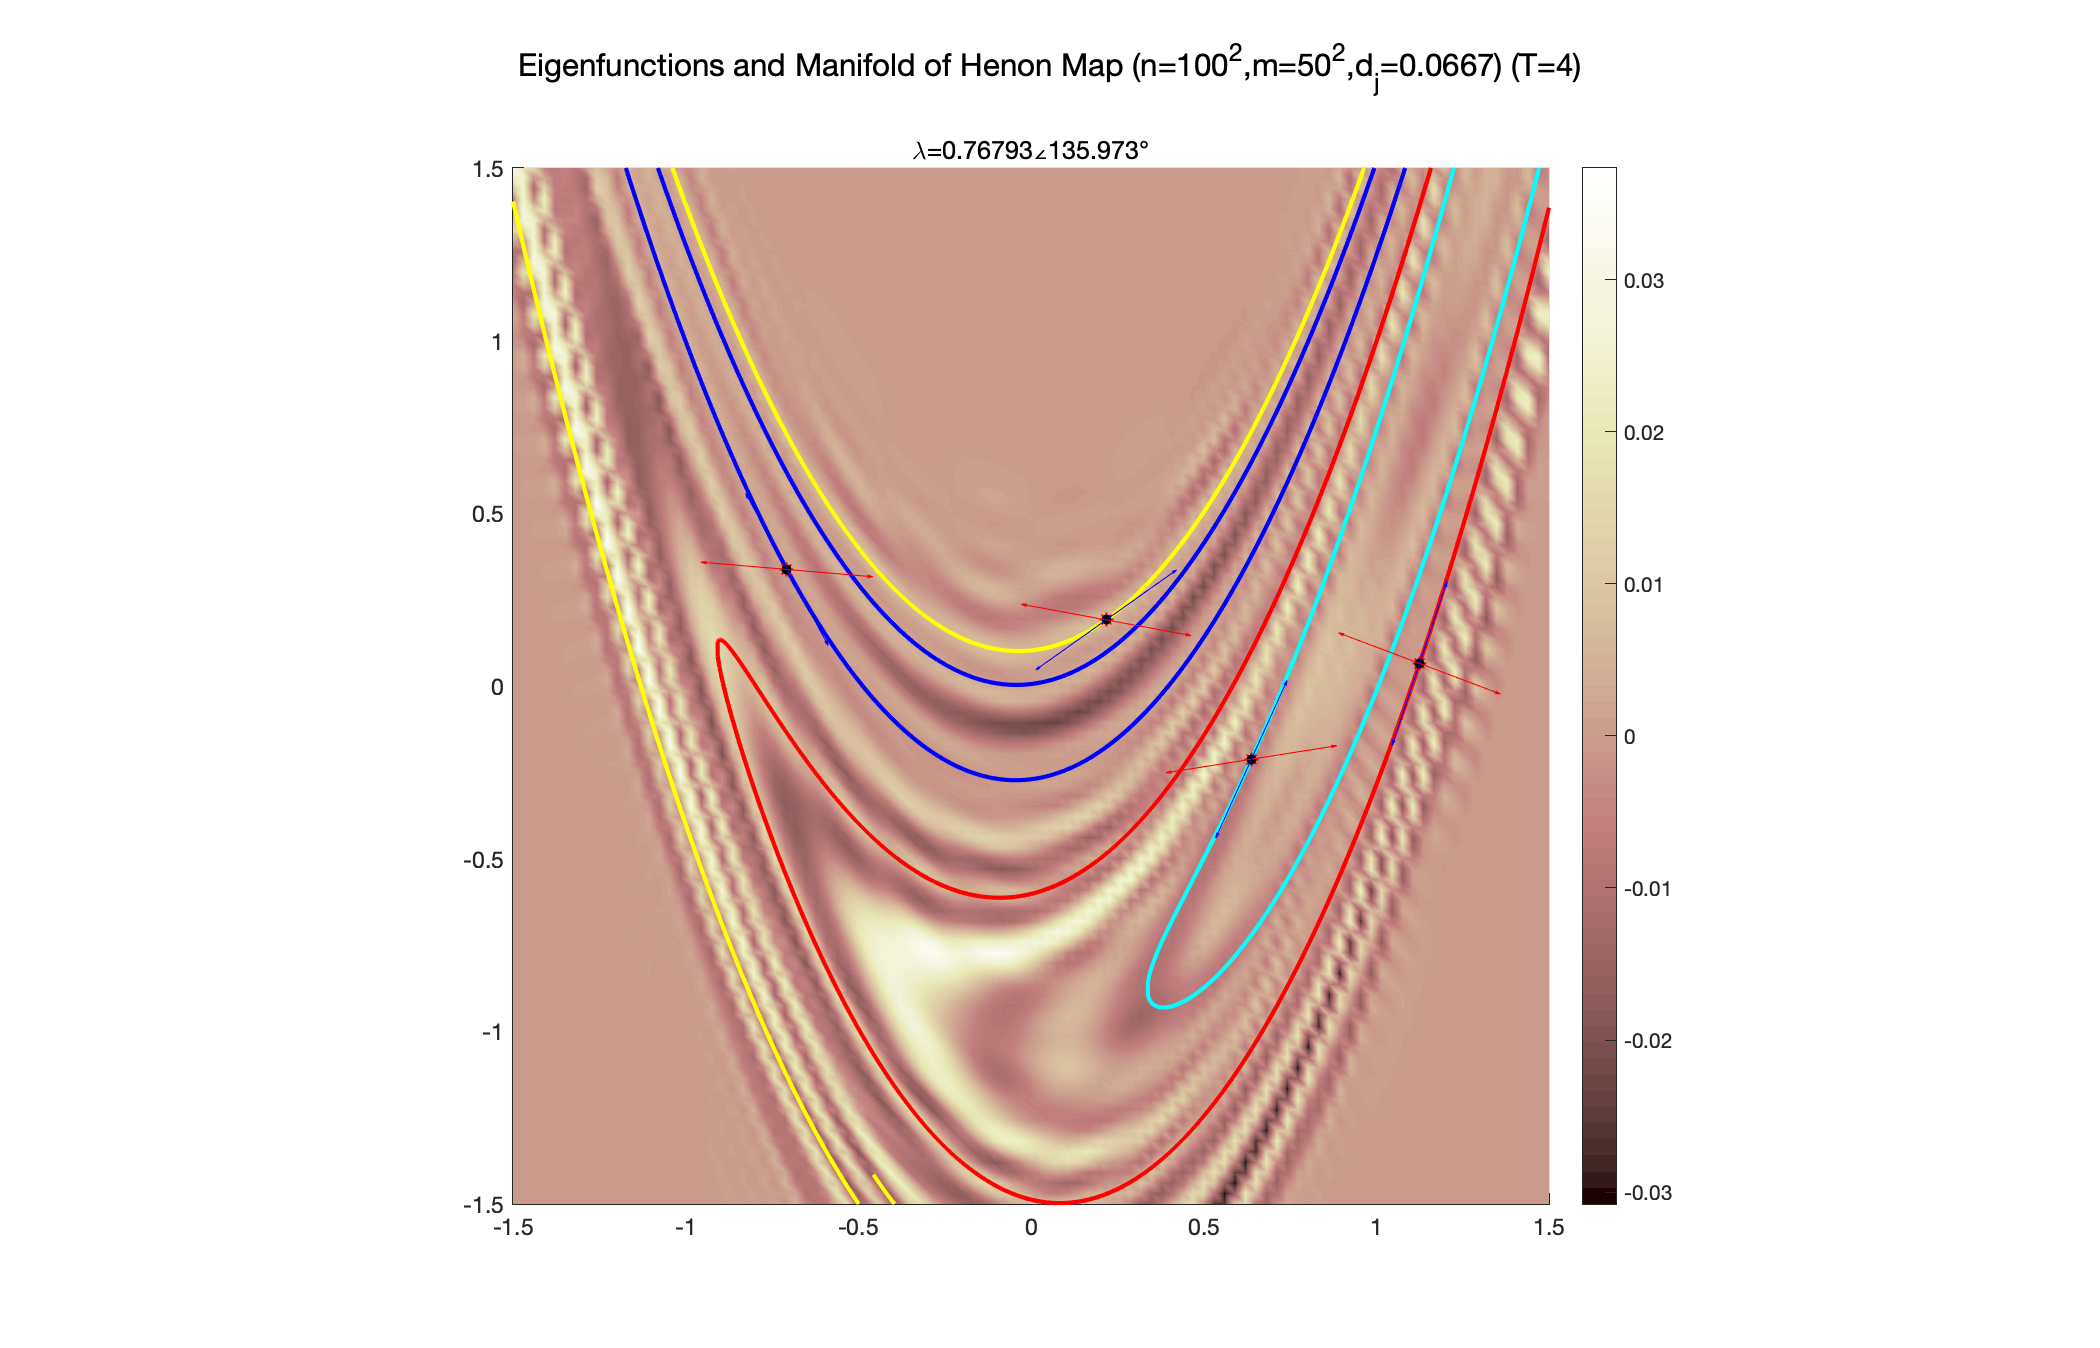
\includegraphics[scale=0.4]{henon/manifold/Henon_eigen_Gauss_manifold_n100m50T4}
    \caption{埃农映射的不稳定流型与本征函数(T=4)}
\end{figure}

\begin{figure}
    \centering
    \subfloat{
      \includegraphics[scale=0.2]{henon/manifold/Henon_eigen_Gauss_manifold_n100m50T7_1}}
    \subfloat{
      \includegraphics[scale=0.2]{henon/manifold/Henon_eigen_Gauss_manifold_n100m50T7_2}}
    \\
    \subfloat{
      \includegraphics[scale=0.2]{henon/manifold/Henon_eigen_Gauss_manifold_n100m50T7_3}}
    \subfloat{
      \includegraphics[scale=0.2]{henon/manifold/Henon_eigen_Gauss_manifold_n100m50T7_4}}
    \\
    \caption{埃农映射的不稳定流型与本征函数(T=7)}
\end{figure}

\subsection{更多的讨论}

\subsection{小结}